\documentclass[10pt,]{book}

% Packages I added.
\usepackage{placeins}
\usepackage{caption}
\usepackage{float}
\floatplacement{figure}{H}
\restylefloat{figure}
\usepackage{makeidx}
\usepackage[nottoc]{tocbibind}
\makeindex
% End of packaged I added.

\usepackage[T1]{fontenc}
\usepackage{lmodern}
\usepackage{amssymb,amsmath}
\usepackage{ifxetex,ifluatex}
\usepackage{fixltx2e} % provides \textsubscript
% use upquote if available, for straight quotes in verbatim environments
\IfFileExists{upquote.sty}{\usepackage{upquote}}{}
\ifnum 0\ifxetex 1\fi\ifluatex 1\fi=0 % if pdftex
  \usepackage[utf8]{inputenc}
\else % if luatex or xelatex
  \ifxetex
    \usepackage{mathspec}
    \usepackage{xltxtra,xunicode}
  \else
    \usepackage{fontspec}
  \fi
  \defaultfontfeatures{Mapping=tex-text,Scale=MatchLowercase}
  \newcommand{\euro}{€}
    \setmainfont{DejaVu Serif}
    \setsansfont{DejaVu Sans}
    \setmonofont[Mapping=tex-ansi]{DejaVu Sans Mono}
\fi
% use microtype if available
\IfFileExists{microtype.sty}{\usepackage{microtype}}{}
\usepackage[margin=1in, paperwidth=7in, paperheight=9in]{geometry}
\usepackage{graphicx}
% Redefine \includegraphics so that, unless explicit options are
% given, the image width will not exceed the width of the page.
% Images get their normal width if they fit onto the page, but
% are scaled down if they would overflow the margins.
\makeatletter
\def\ScaleIfNeeded{%
  \ifdim\Gin@nat@width>\linewidth
    \linewidth
  \else
    \Gin@nat@width
  \fi
}
\makeatother
\let\Oldincludegraphics\includegraphics
{%
 \catcode`\@=11\relax%
 \gdef\includegraphics{\@ifnextchar[{\Oldincludegraphics}{\Oldincludegraphics[width=\ScaleIfNeeded]}}%
}%
\ifxetex
  \usepackage[setpagesize=false, % page size defined by xetex
              unicode=false, % unicode breaks when used with xetex
              xetex]{hyperref}
\else
  \usepackage[unicode=true]{hyperref}
\fi
\hypersetup{breaklinks=true,
            bookmarks=true,
            pdfauthor={Jim Lehmer},
            pdftitle={Jim's Ten Steps to Linux Survival},
            colorlinks=true,
            citecolor=blue,
            urlcolor=blue,
            linkcolor=magenta,
            pdfborder={0 0 0}}
\urlstyle{same}  % don't use monospace font for urls
\usepackage[normalem]{ulem}
% avoid problems with \sout in headers with hyperref:
\pdfstringdefDisableCommands{\renewcommand{\sout}{}}
\setlength{\parindent}{0pt}
\setlength{\parskip}{6pt plus 2pt minus 1pt}
\setlength{\emergencystretch}{3em}  % prevent overfull lines
\setcounter{secnumdepth}{0}

\title{Jim's Ten Steps to Linux Survival}
\author{Jim Lehmer}
\date{}

% Overriding commands.
\renewcommand{\chaptername}{Step}
\renewcommand{\contentsname}{Steps}
\numberwithin{figure}{chapter}
% End of overriding commands.

\begin{document}
\maketitle

{
\hypersetup{linkcolor=black}
\setcounter{tocdepth}{3}
\tableofcontents
}

% Add list of figures.
{
\listoffigures
}
% End of list of figures.

\ifxetex
\section*{} \pagestyle{empty}

\begin{figure}[!htbp]

\includegraphics{./images/Merv.jpg}%
\caption*{Merv sez, "Don't panic."}%
\end{figure}

\cleardoublepage
By James Lehmer \newline
\newline
v0.3 \newline
\newline

\begin{figure}[!htbp]
\centering

\includegraphics{./images/cc-by-sa.png}%
\caption*{Creative Commons Attribution-ShareAlike 4.0 International License}%
\end{figure}

\emph{Jim's Ten Steps to Linux Survival} by James Lehmer is licensed
under a \href{http://creativecommons.org/licenses/by-sa/4.0/}{Creative
Commons Attribution-ShareAlike 4.0 International License}.
\pagestyle{headings} \else

\begin{figure}[htbp]
\centering

\includegraphics{./images/Merv.jpg}
\caption{Merv sez, ``Don't panic.''}
\end{figure}

By James Lehmer v0.4 {Jim's Ten Steps to Linux Survival} by {James
Lehmer} is licensed under a Creative Commons Attribution-ShareAlike 4.0
International License.

\fi

\textbf{Dedicated to my first three technical mentors} - Jim Proffer,
who taught me digging deeper was fun and let me do so (often in
production). Jerry Wood, who taught me to stop and think (and once
called me an ``inveterate toolmaker'' in a review). And Kim Manchak, who
let me be more than he hired me to be (and continues to be a great chess
opponent). Thank you, gentlemen. I've tried to pay it forward. This book
is part of that.

\ifxetex
\setcounter{chapter}{-2} \fi

\chapter{Introduction}\label{introduction}

\begin{quote}
\emph{``And you may ask yourself, `Well, how did I get here?'\,''} -
Talking Heads (\emph{Once in a Lifetime})
\end{quote}

This is my little ``Linux and Bash in 10 steps'' guide. It's based
around what I consider the essentials for \sout{floundering around}
acting like I know what I'm doing in Linux, BSD and ``UNIX-flavored''
systems and looking impressive among people who have only worked on
Windows in the GUI. Your ``10 steps'' may be different than mine and
that's fine, but this list is mine.

I said ten things, but I lied, because history is really important, so
we will start at step \#0. And since this is before even that I guess
that means this is a 12-step program\ldots{}

Here is what we'll cover in the rest of this book:

\begin{enumerate}
\def\labelenumi{\arabic{enumi}.}
\setcounter{enumi}{-1}
\item
  \hyperref[step-0.-some-history]{\textbf{Some History}} -- UNIX
  vs.~BSD, System V vs. BSD, Linux vs.~BSD, POSIX, ``UNIX-like,''
  Cygwin, and why any of this matters now, ``Why does this script off
  the internet work on this system and not on that one?''
\item
  \hyperref[step-1.-come-out-of-your-shell]{\textbf{Come Out of Your
  Shell}} -- \texttt{sh} vs. \texttt{ash} vs. \texttt{bash}
  vs.~everything else, ``REPL'', interactive vs.~scripts, command
  history, tab expansion, environment variables and ``A path! A path!''
\item
  \hyperref[step-2.-file-under-directories]{\textbf{File Under
  ``Directories''}} -- \texttt{ls}, \texttt{mv}, \texttt{cp},
  \texttt{rm} (\texttt{-rf *}), \texttt{cat},
  \texttt{chmod}/\texttt{chgrp}/\texttt{chown} and everyone's favorite,
  \texttt{touch}.
\item
  \hyperref[step-3.-finding-meaning]{\textbf{Finding Meaning}} -- the
  \texttt{find} command in all its glory. Probably the single most
  useful command in ``UNIX'' (I think).
\item
  \hyperref[step-4.-grokking-grep]{\textbf{Grokking \texttt{grep}}} --
  and probably gawking at \texttt{awk} while we are at it, which means
  regular expressions, too. Now we have two problems.
\item
  \hyperref[step-5.-just-a-series-of-pipes]{\textbf{``Just a Series of
  Pipes''}} -- \texttt{stdin}/\texttt{stdout}/\texttt{stderr},
  redirects, piping between commands.
\item
  \hyperref[step-6.-vi]{\textbf{\texttt{vi}}} (had to be \#6, if you
  think about it) -- how to stay sane for 10 minutes in \texttt{vi}.
  Navigation, basic editing, find, change/change-all, cut and paste,
  undo, saving and canceling. Plus easier alternatives like
  \texttt{nano}, and why \texttt{vi} still matters.
\item
  \hyperref[step-7.-the-whole-wide-world]{\textbf{The Whole Wide World}}
  -- \texttt{curl}, \texttt{wget}, \texttt{ifconfig}, \texttt{ping},
  \texttt{ssh}, \texttt{telnet}, \texttt{/etc/hosts} and email before
  Outlook.
\item
  \hyperref[step-8.-the-man-behind-the-curtain]{\textbf{The Man Behind
  the Curtain}} - \texttt{/proc}, \texttt{/dev}, \texttt{ps},
  \texttt{/var/log}, \texttt{/tmp} and other things under the covers.
\item
  \hyperref[step-9.-how-do-you-know-what-you-dont-know-man]{\textbf{How
  Do You Know What You Don't Know, \texttt{man}?}} -- \texttt{man},
  \texttt{info}, \texttt{apropos}, Linux Documentation Project, Debian
  and Arch guides, StackOverflow and the dangers of searching for
  ``\texttt{man find}'' or ``\texttt{man touch}'' on the internet.
\item
  \hyperref[step-10.-and-so-on]{\textbf{And So On}} - \texttt{/etc},
  starting and stopping services,
  \texttt{apt-get}/\texttt{rpm}/\texttt{yum}, and more.
\end{enumerate}

Plus \hyperref[appendices]{some stuff} at the end to tie the whole room
together.

\section{Batteries Not Included}\label{batteries-not-included}

It should be obvious that there is \textbf{\emph{plenty}} that is not
covered:

\begin{itemize}
\item
  \textbf{System initialization} - besides, the whole ``UNIX'' world is
  in flux right now over system initialization architecture and the
  shift from \href{https://en.wikipedia.org/wiki/Init}{``init''} scripts
  to \href{https://en.wikipedia.org/wiki/Systemd}{\texttt{systemd}}.
\item
  \textbf{Scripting logic} - scripting, logic constructs
  (\texttt{if}/\texttt{fi}, \texttt{while}/\texttt{done}, and the like).
\item
  \textbf{Desktops} - X Windows and the plethora of desktop environments
  like GNOME, KDE, Cinnamon, Mate, Unity and on and on. This is where
  ``UNIX'' systems get the farthest apart in terms of interoperability,
  settings and customization.
\item
  \textbf{Servers} - setting up or configuring web servers like Apache
  or node, email servers like dovecot, Samba servers for file shares,
  and so on.
\item
  \textbf{Security} - other than the simple basics of the file system
  security model.
\end{itemize}

Plus so much more. Again, this is not meant to be exhaustive, but to
help someone whose system administration experience has been limited to
``Next-Next-Next-Finish'' installs and filling in text boxes in wizards
on Windows.

\section{Please, Give Generously}\label{please-give-generously}

That said, if you find something amiss in here - a typo, a misconception
or mistake, or a command or parameter you \textbf{\emph{really, really,
really}} think should be in here even though I said I am not trying to
be exhaustive, feel free to
\href{https://github.com/dullroar/ten-steps-to-linux-survival.git}{clone
it from GitHub}, make your changes and send me a \texttt{git pull}
request. Or you can try to
\href{https://github.com/dullroar/ten-steps-to-linux-survival/issues?q=is\%3Aopen+is\%3Aissue}{file
it as an issue} and I'll see how I feel that day.

\section{Why?}\label{why}

Because I work in a primarily Windows-oriented shop, and I seem to be
``the guy'' that everyone comes to when they need help on a Linux or
related system. I don't count myself a Linux guru (\textbf{\emph{at
all}}), but I have been running it since 1996 (Slackware on a laptop
with 8MB of memory!), and have worked on or run at home various ports
and flavors and and versions and distros of ``UNIX'' over the years,
including:

\begin{itemize}
\item
  \textbf{AIX}
\item
  \textbf{FreeBSD}
\item
  \textbf{HP/UX}
\item
  \textbf{Linux} - literally more distros than I can count or remember,
  but at least Debian, Fedora, Yellow Dog, Ubuntu/Kubuntu/Xubuntu, Mint,
  Raspbian, Gentoo, Red Hat and of course the venerable Slackware.
\item
  \textbf{Solaris}
\item
  \textbf{SunOS}
\end{itemize}

\ldots{}on various machines and machine architectures from mighty Sun
servers to generic ``Intel'' VMs down to Raspberry Pis (plus an original
``wedge'' iMac running as a kitchen kiosk long after its ``Best by''
date and OS/9's demise, thanks to Yellow Dog Linux).

All that while also working on MVS, VSE, OS/2, DOS since 3.x, Windows
since 1.x, etc., etc. I don't think I am special when I list all that -
there are lots of people with my level of experience \textbf{\emph{and
better}}, especially in commercial software engineering. I am just one
of them.

But for some reason there are many places, especially in small and
medium business (SMB) environments, where the ``stack'' tends to be more
purely Microsoft because it keeps things simpler and cheaper for the
(smaller) staff. I work in such a place. The technical staff is quite
competent, but when they bump up against systems whose primary ``user
interface'' for system administration is a command prompt and some
scripts, they panic.

This is my attempt to help my co-workers by saying:

\begin{quote}
\emph{``Don't panic.''} - Douglas Adams (\emph{Hitchhiker's Guide to the
Galaxy})
\end{quote}

It started out as a proposal I made a few weeks ago to develop a ``lunch
and learn'' session of about 60-90 minutes of what I considered to be
``a Linux survival guide.'' The list in the \emph{Introduction} above is
based on my original email proposal. The audience would be entirely
technical, primarily ``IT'' (Windows/Cisco/VMWare/Exchange/SAN admins).

My goal is not to get into scripting or system setup and hardening or
the thousand different ways to slice a file. Instead, the scenario I see
in my head is for one of the participants in that ``lunch and learn,''
armed with that discussion and having glanced through this book, to be
better able to survive if dropped into the jungle with:

\begin{quote}
\emph{``The main www site is down, and all the people who know about it
are out. It's running on some sort of Linux, I think, and the
credentials and IP address are scrawled on this sticky note. Can you get
in and poke around and see if you can figure it out?''} - your boss
(next Tuesday morning)
\end{quote}

Well, as I started to type out my notes of what I considered to be
``essential,'' they just kept growing and growing. And now, some nights,
weekends and lunch hours gone, this is what you see as the result. I
figure the slides will be easier to prepare for that ``lunch and
learn,'' now that I have the ``notes''!

\section{Caveat Administrator}\label{caveat-administrator}

Even so, anything like this is incomplete. Anyone knowledgable of Linux
will probably splutter their coffee into their neckbeard at least once a
chapter because I don't mention a parameter on a command or an entire
subject at all! And that's right - because this ``survival guide'' is
already long enough.

This book is not meant to be an authoritative source, but instead a
\href{https://en.wikipedia.org/wiki/Fake_book}{``fake book''} for
getting up and running \textbf{\emph{quickly}} with the sheer basics,
plus knowing where to go for help. It is not a replacement for reading
the real documentation and doing research and testing, especially in
production! But hopefully it will help get you through that ``Can you
get in and poke around and see if you can figure it out?'' scenario,
above. And if Linux should start becoming more of your job, maybe this
will help as a gentle push toward ``RTFM'' along with thinking in ``The
UNIX Way.''

\textbf{WARNING:} \textbf{\emph{Many of the commands in this book can
alter your system and possibly damage it.}} Obvious candidates include
the file system commands like \texttt{rm}, the \texttt{vi} editor
(obviously), and some of the ``system admin'' commands mentioned later,
including system and service restarts. Use your common sense plus the
various resources for documentation mentioned in this book to make sure
you aren't doing anything destructive to your system, especially in
production. \textbf{\emph{You have been warned!}}

\section{Conventions}\label{conventions}

If a command, file name or other ``computer code'' is shown in-line in a
sentence, it will appear in a fixed-width font, e.g.,
\texttt{ls -{}-recursive *.txt}.

If a command and its output, script code or something else is shown in a
block, it will appear like this:

\begin{verbatim}
~ $ ps -AH
  PID TTY          TIME CMD
    2 ?        00:00:00 kthreadd
    3 ?        00:00:00   ksoftirqd/0
    5 ?        00:00:00   kworker/0:0H
    7 ?        00:00:19   rcu_sched
    8 ?        00:00:04   rcuos/0
    9 ?        00:00:09   rcuos/1
   10 ?        00:00:07   rcuos/2
...and so on...
\end{verbatim}

\textbf{Note:} The examples in this book typically show something like
\texttt{\textasciitilde{} \$} or \texttt{\#} before the command (the
latter especially when logged in as \texttt{root} or running under
\texttt{csh}). These ``command prompts'' are set in \texttt{bash} via
the
\href{https://www.linux.com/learn/docs/ldp/443-bash-prompt-howto}{\texttt{PS1}
environment variable} and are not meant to be typed in as part of the
command.

Samples may also appear in a screenshot like this:

\ifxetex

\begin{figure}[!htbp]
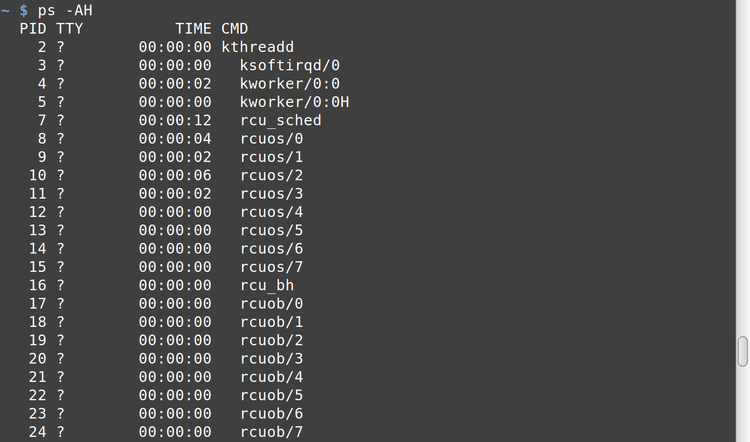
\includegraphics{./images/ps-AH.png}%
\caption{Sample command}%
\end{figure}

\else

\begin{figure}[htbp]
\centering
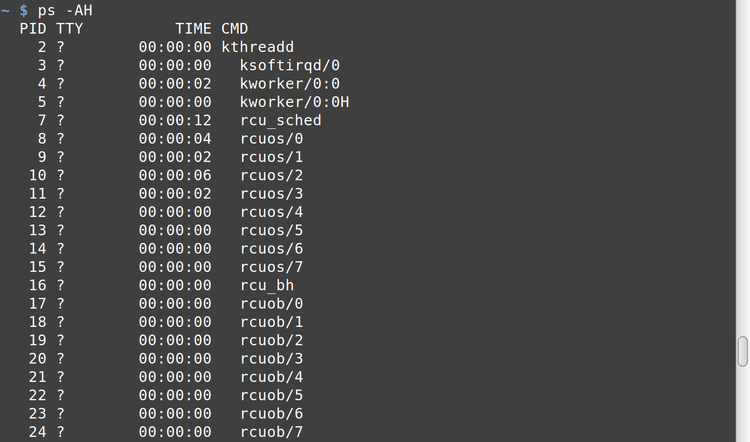
\includegraphics{./images/ps-AH.png}
\caption{Sample command}
\end{figure}

\fi

\chapter{Some History}\label{some-history}

\textbf{\emph{UNIX vs.~BSD, System V vs.~BSD, Linux vs.~BSD, POSIX,
``UNIX-like,'' Cygwin, and why any of this matters now. ``Why does this
script off the internet work on this system and not on that one?''}}

\begin{quote}
\emph{``That men do not learn very much from the lessons of history is
the most important of all the lessons of history.''} - Aldous Huxley
\end{quote}

UNIX and its successors such as Linux have a long history reaching into
the depths of time:

\begin{itemize}
\item
  \textbf{Prehistory} - late 1960s, Nixon, Vietnam, Woodstock, Moon
  landing, \href{https://en.wikipedia.org/wiki/Multics}{Multics} at MIT,
  GE and Bell Labs.
\item
  \textbf{In the beginning} - early 1970s, Nixon drags on, Watergate,
  Bell Labs, \href{https://en.wikipedia.org/wiki/Ken_Thompson}{Thompson}
  \& \href{https://en.wikipedia.org/wiki/Dennis_Ritchie}{Ritchie},
  \href{https://en.wikipedia.org/wiki/History_of_Unix}{UNIX},
  \index{UNIX} blah blah blah\ldots{}
\item
  \textbf{More Trouble From Berkeley} - late 1970s, Carter, disco, Iran
  hostages, UC Berkely releases the
  \href{https://en.wikipedia.org/wiki/Berkeley_Software_Distribution}{Berkeley
  Software Distribution} (BSD), \index{BSD} a port based on the Bell
  Labs UNIX. Let the forking begin!
\item
  \textbf{Goes commercial} - 1980s, Reagan, Iran Contra, \emph{E.T.},
  AT\&T releases
  \href{https://en.wikipedia.org/wiki/UNIX_System_V}{System V}
  \index{System V} as first commercial UNIX. From the same background as
  Bell Labs UNIX, but evolved with subtle and not so subtle differences
  in approaches to command syntax, networking and much more. It is this
  release and AT\&T's copyrights that are the basis of all the
  SCO-vs-Linux lawsuits 2-3 decades later.
\item
  \textbf{Explosion of ``UNIX''} -late 1980s/early 1990s, Bush I, Berlin
  Wall falls, Gulf War I, proliferation of proprietary (and different)
  ``UNIX'' platforms:

  \begin{itemize}
  \itemsep1pt\parskip0pt\parsep0pt
  \item
    \textbf{HP HP-UX}
  \item
    \textbf{Sun SunOS} - BSD flavor.
  \item
    \textbf{Sun Solaris} - System V flavor. Now Oracle Solaris.
  \item
    \textbf{IBM AIX}
  \item
    \textbf{SGI IRIX}
  \item
    \textbf{\ldots{}and many, many more!} - although mostly all that's
    left now is HP-UX, AIX and Solaris.
  \end{itemize}
\item
  \textbf{Linux} - 1991+, Clinton I, grunge, \emph{Titanic},
  \href{https://en.wikipedia.org/wiki/Linus_Torvalds}{Linus Torvalds}
  releases a project called
  \href{https://en.wikipedia.org/wiki/Linux}{Linux} \index{Linux} based
  on \href{https://en.wikipedia.org/wiki/MINIX}{MINIX} (and hence why
  Linus says Linux is pronounced like ``MINIX'' and not like ``Linus'').
\item
  \textbf{Proliferation of the BSDs} - mid-to-late 1990s, still Clinton
  I, Monicagate, Kosovo, various ports of BSD including
  \href{https://en.wikipedia.org/wiki/NetBSD}{NetBSD}, \index{NetBSD}
  \href{https://en.wikipedia.org/wiki/FreeBSD}{FreeBSD} \index{FreeBSD}
  and \href{https://en.wikipedia.org/wiki/OpenBSD}{OpenBSD},
  \index{OpenBSD} all happen in the same time frame as Linux. Like Linux
  distros, each has its own focus and prejudices, some of which are
  distinctly ``anti-Linux.'' The ``big three'' are all still in heavy
  use today, especially among ISPs. The perception is still out there
  among a generation of sysadmins that Linux is for the desktop and BSDs
  for servers, but that reality shifted a long time ago.
\item
  \textbf{Ports of call} - 2000+, Bush II \& Obama, Afghanistan \& Gulf
  War 2, lots of cross-porting of everything open source. However,
  \href{https://en.wikipedia.org/wiki/Open-source_license}{licenses
  matter}, and
  \href{https://en.wikipedia.org/wiki/Comparison_of_free_and_open-source_software_licenses}{there
  sure are a lot of them}. While it has settled down some with the
  dismissal of the SCO lawsuit, intellectual property remains a problem
  area in open source, even as its use has exploded.
\end{itemize}

\textbf{Q:} So, what's Linux? Or BSD? Or even UNIX?

\textbf{A:} Depends on who you're asking and in what context!

Hence, for the rest of this text I will tend to talk somewhat
interchangeably about ``Linux'' and ``UNIX'' and the like. When it
matters, I will mention which OS I am discussing by name, but often I
will use ``UNIX'' (in quotes) to mean anything in the ``family tree'' of
the original Bell Labs offspring, or that ``acts like,'' well, UNIX.

To further muddy the waters, there have been multiple attempts to
``standardize'' whatever it is this thing is called:

\begin{itemize}
\itemsep1pt\parskip0pt\parsep0pt
\item
  \href{https://en.wikipedia.org/wiki/POSIX}{\textbf{POSIX}} -
  \index{POSIX} a de jure set of standards created in the 1980s and
  1990s to try to bring order to the chaos that was commercial
  UNIX-flavored operating systems of the time. It worked. Sorta.
  Especially once the US government started wanting systems to be
  ``POSIX-compliant.''
\end{itemize}

\textbf{Note:} No system runs POSIX, they all are ``similar but
different.'' Even Windows can claim to be POSIX in some respects (and
has an installable POSIX subsystem), but that doesn't mean
POSIX-compliant code will run there unchanged.

\begin{itemize}
\item
  \href{https://en.wikipedia.org/wiki/GNU_Project}{\textbf{GNU Project}}
  - \href{https://en.wikipedia.org/wiki/Richard_Stallman}{Richard
  Stallman} founded the
  \href{https://en.wikipedia.org/wiki/Free_Software_Foundation}{Free
  Software Foundation} (FSF) and GNU project \index{GNU} in the
  mid-1980s, \textbf{\emph{long}} before Linux (GNU = ``GNU's Not
  Unix''). The GNU project delivers
  \href{https://www.gnu.org/software/software.html}{a suite of programs
  and tools}, many of which are used in both Linux and BSD variants as
  de facto standards.
\item
  \textbf{Various Linux Efforts} - there have also been various
  movements over the years, some more successful than others, to
  ``standardize'' Linux or some part of it, such as the file system
  layout, the \texttt{init} system, documentation, and now even what is
  part of the most basic ``core OS'' for things like better
  containerization.
\end{itemize}

\section{Why Does This Matter?}\label{why-does-this-matter}

Because there are various ``flavors'' of commands and tools, based on
whether you're dealing with a System V (Linux) or BSD (Free/Net/Open)
descendant. Some of the OS versions are strong in security, or
networking, or as a desktop. Certain things are ``built-in'' to the
operating system but most are installed as packages, and depending on
the source of the package it may or may not work correctly on another
``UNIX'' system without effort.

It is similar to the history and relationship between
\texttt{COMMAND.EXE} in DOS and \texttt{CMD.EXE} in Windows 10, where
this would work in both:

\begin{verbatim}
COPY A.TXT B.TXT
\end{verbatim}

But only the later, network-and-NTFS-aware \texttt{CMD.EXE} could
handle:

\begin{verbatim}
COPY "My 2015 Tax Returns.pdf" \\MyServer\Finances\.
\end{verbatim}

In UNIX-land over time these differences seem to be getting better, but
there are still ``gotchas,'' often involving the differences in open
source licenses in the underlying code. There are fundamental
differences and assumptions between the ``GNU'' and ``GPL'' licenses on
the one side and ``MIT'' and ``BSD'' licenses on the other. I am not a
lawyer, but I would summarize:

\begin{itemize}
\item
  \textbf{FSF/GNU/GPL} - mostly concerned with keeping open source
  ``open,'' that is sharable and modifiable by all.
\item
  \textbf{BSD \& MIT} - more focused on letting anyone do anything to
  the code as long as the original author is acknowledged and liability
  released.
\end{itemize}

The best thing is to be vaguely aware of this history and licenses and
if something isn't available on a certain platform or if a command isn't
taking a specific parameter to search for variants.

For example, note the differences in command line parameters and output
between showing all processes with the
\href{http://linux.die.net/man/1/ps}{\texttt{ps}} (\emph{process})
command on a Linux system, in this case Linux Mint:

\begin{verbatim}
$ ps -AH
  PID TTY          TIME CMD
    2 ?        00:00:00 kthreadd
    3 ?        00:00:00   ksoftirqd/0
    5 ?        00:00:00   kworker/0:0H
    7 ?        00:00:19   rcu_sched
    8 ?        00:00:04   rcuos/0
    9 ?        00:00:09   rcuos/1
   10 ?        00:00:07   rcuos/2
...and so on...
\end{verbatim}

\ldots{}versus on a FreeBSD system at my ISP, where \texttt{csh} is the
default shell:

\begin{verbatim}
%ps -ax
  PID  TT  STAT      TIME COMMAND
73591  ??  S      0:00.03 sshd: myuser@ttyp1 (sshd)
79503  ??  S      0:00.07 dovecot/imap
80065  ??  S      0:00.05 dovecot/imap
73593  p1  Ss     0:00.02 -csh (csh)
90737  p1  RN+    0:00.00 ps -ax
\end{verbatim}

To make things even more confusing, the Linux version of \texttt{ps} has
been written to understand the BSD-style syntax and flags, too!

\section{Panic at the Distro}\label{panic-at-the-distro}

Remember that ``Linux,'' FreeBSD, OpenBSD and NetBSD are all really just
OS kernels, boot loaders, drivers and enough functionality to get a
computer up and running. Most functionality comes via other
``packages.'' From almost the beginning there have been alternative
approaches to both what packages should (and should not) be included, as
well as how best to manage the installing, updating and removal of those
packages.

In the BSD world each major port has its own approach. In the Linux
world the job of deciding all this and putting it all together falls to
distributions or ``distros.'' \index{Linux distros} These have evolved
over time into a series of
\href{https://en.wikipedia.org/wiki/Linux_distribution\#Popular_distributions}{``families''}
based in large part around the
\href{https://en.wikipedia.org/wiki/Package_manager}{package management
tool} predominantly used:

\begin{itemize}
\item
  \textbf{\texttt{apt-get}, \texttt{dpkg} and \texttt{.deb} files} -
  \index{apt-get} \index{dpkg}
  \href{https://en.wikipedia.org/wiki/Debian}{Debian} flavors, such as
  \href{https://en.wikipedia.org/wiki/Ubuntu_\%28operating_system\%29}{Ubuntu}
  and \href{https://en.wikipedia.org/wiki/Linux_Mint}{Mint} (Mint is
  currently my desktop Linux of choice, Debian my preferred server OS,
  but both solely based on familiarity).
\item
  \textbf{\texttt{pacman}} - \index{pacman}
  \href{https://en.wikipedia.org/wiki/Arch_Linux}{Arch} flavors.
\item
  \textbf{\texttt{rpm} and \texttt{yum}} - \index{rpm} \index{yum} Red
  Hat flavors, such as
  \href{https://en.wikipedia.org/wiki/Fedora_\%28operating_system\%29}{Fedora},
  \href{https://en.wikipedia.org/wiki/Red_Hat_Enterprise_Linux}{Red Hat
  Enterprise} and \href{https://en.wikipedia.org/wiki/CentOS}{CentOS}.
\item
  \textbf{Source code} -
  \href{https://en.wikipedia.org/wiki/Gentoo_Linux}{Gentoo} tends to be
  a ``compile from scratch'' environment, much like
  \href{https://en.wikipedia.org/wiki/FreeBSD_Ports}{FreeBSD}.
\item
  \textbf{``Tar balls''} - source code or binaries delivered via
  archived and zipped directories. Common on
  \href{https://en.wikipedia.org/wiki/Slackware}{Slackware}, some
  others.
\end{itemize}

\section{Get Embed With Me}\label{get-embed-with-me}

A lot of firmware in embedded devices is based on some sort of ``UNIX''
flavor. Networking gear at both the consumer and enterprise level,
storage devices and so on all tend to run something that ``looks like''
UNIX at some level. Of course, as to what's actually available, who
knows? If you can get a shell (command prompt) the best thing to do is
see what works.

\section{Cygwin}\label{cygwin}

\href{http://cygwin.com/}{Cygwin} \index{Cygwin} is an interesting
beast. It is a DLL for Windows that implements most of the POSIX and
related UNIX-like ``system API calls'' for programming, and then is also
a series of ported open source packages, including shells, utilities and
even desktop environments, all \textbf{\emph{recompiled}} to run on
Windows as long as the Cygwin DLL is accessible. Like a Linux distro it
has an installer that is a ``package manager,'' and if a package isn't
available, you can usually recompile the source code using Cygwin.

You cannot run Linux or BSD binaries on Cygwin without recompiling them
first. \textbf{However}, you can often run \textbf{\emph{scripts}} from
a Linux environment on Cygwin with little or no tweaking. Which means
you can then take advantage of a lot of excellent open source tools
simply by installing their packages in Cygwin and running scripts
against them.

Ultimately, though, Cygwin is of limited use, basically for getting to
some open source tools on Windows without having to set up a Linux box.
You can do a lot of amazing things with Cygwin with enough effort
(including running X and a desktop environment like GNOME!), but at some
point why not expend that effort in standing up a ``real'' Linux
(virtual) machine anyway?

\chapter{Come Out of Your Shell}\label{come-out-of-your-shell}

\textbf{\emph{\texttt{sh} vs. \texttt{ash} vs. \texttt{bash}
vs.~everything else, ``REPL'', interactive vs.~scripts, command history,
tab expansion, environment variables and ``A path! A path!''}}

\begin{quote}
\emph{``If you hold a shell up to your ear, you can hear the OS.''} - me
\end{quote}

To avoid getting all pedantic, I am just going to define a shell as an
environment in which you can execute commands. People tend to think of a
shell as a ``command prompt,'' but you can run a shell without running a
command prompt, but not vice versa - an interactive command prompt is an
instance of a shell environment almost by definition.

Examples of shells:

\begin{itemize}
\item
  \href{https://technet.microsoft.com/en-us/library/cc754340.aspx}{\textbf{\texttt{CMD.EXE}}}
  - yes, Windows has a shell.
\item
  \href{https://technet.microsoft.com/en-us/library/ms714469\%28v=VS.85\%29.aspx}{\textbf{\texttt{PowerShell.exe}}}
  - in fact, it has at least two!
\end{itemize}

In UNIX-land:

\begin{itemize}
\item
  \href{https://en.wikipedia.org/wiki/Bourne_shell}{\textbf{\texttt{sh}}}
  - the ``original'' Bourne shell in UNIX, which spawned:

  \begin{itemize}
  \item
    \href{https://en.wikipedia.org/wiki/Almquist_shell}{\textbf{\texttt{ash}}}
    - Almquist shell.

    \begin{itemize}
    \itemsep1pt\parskip0pt\parsep0pt
    \item
      \textbf{\texttt{dash}} - Debian Almquist shell (replaced
      \texttt{ash} in Debian)
    \end{itemize}
  \item
    \href{https://en.wikipedia.org/wiki/Bash_\%28Unix_shell\%29}{\textbf{\texttt{bash}}}
    - Bourne-again shell (get it?), the ``standard'' Linux shell.
  \item
    \href{https://en.wikipedia.org/wiki/Korn_shell}{\textbf{\texttt{ksh}}}
    - Korn shell.
  \item
    \href{https://en.wikipedia.org/wiki/Z_shell}{\textbf{\texttt{zsh}}}
    - Z shell.
  \end{itemize}
\item
  \href{https://en.wikipedia.org/wiki/C_shell}{\textbf{\texttt{csh}}} -
  C shell, historically it is the default shell on BSD systems (although
  there are arguments on why you should
  \href{http://www.faqs.org/faqs/unix-faq/shell/csh-whynot/}{\textbf{\emph{never
  use it}}}).
\item
  \textbf{\ldots{}and many more!} -
  \href{https://en.wikipedia.org/wiki/Unix_shell\#Shell_categories}{tons,
  really}.
\end{itemize}

Most Linux distros use \texttt{bash}, but the BSDs are all over the
place. We're going to assume \texttt{bash} for the rest of this
tutorial. With few modifications, anything in the \texttt{sh} hierarchy
above can usually run in the other members of the same tree.

\section{\texttt{bash} Built-Ins}\label{bash-built-ins}

Every shell has some ``built-in'' commands that are implemented as part
of the shell and not as an external command or program, and
\texttt{bash} has its share, as shown by running the
\href{http://linux.die.net/man/1/help}{\texttt{help}} command in a
\texttt{bash} terminal:

\ifxetex

\begin{figure}[!htbp]
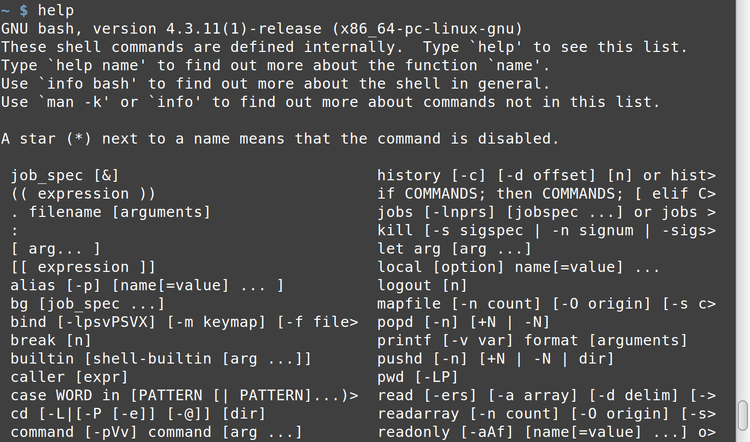
\includegraphics{./images/help.png}%
\caption{Built-in commands}%
\end{figure}

\else

\begin{figure}[htbp]
\centering
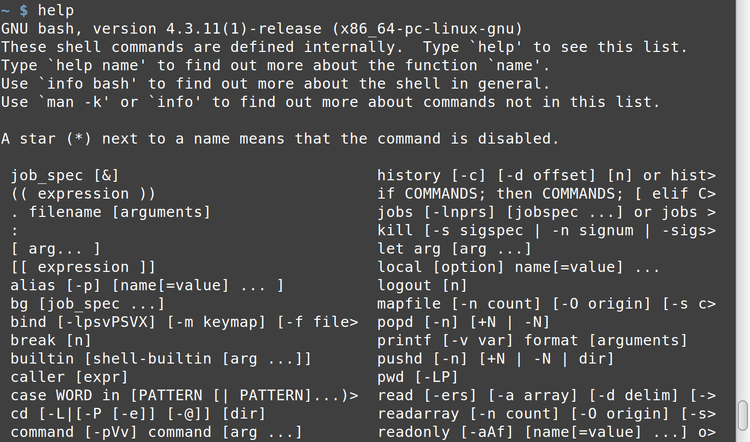
\includegraphics{./images/help.png}
\caption{Built-in commands}
\end{figure}

\fi

Why does this matter? Because if you are in an environment and something
as fundamental as \texttt{echo} isn't working, you may not be working in
a shell that is going to act like a ``\texttt{sh}'' shell.
\textbf{\emph{In general}}, \texttt{sh}, \texttt{ash}, \texttt{bash},
\texttt{dash} and \texttt{ksh} all act similarly enough that you don't
care, but sometimes you may have to care. Knowing if you are on a
\texttt{csh} variant or even something more esoteric can be key.

Pay attention to the first line in script files, which will typically
have a
\href{https://en.wikipedia.org/wiki/Shebang_\%28Unix\%29}{``shebang''}
line that looks like this:

\begin{verbatim}
#!/bin/bash
\end{verbatim}

In this case we know the script is expecting to be executed by
\texttt{bash}, and in fact should throw an error if \texttt{/bin/bash}
doesn't exist. Note that on some systems:

\begin{verbatim}
#!/bin/sh
\end{verbatim}

\ldots{}is pointing to an alias of \texttt{bash}, and on some it is a
different implementation of the original \texttt{sh} command, such as
\texttt{ash} or \texttt{dash}. Now you know what to google if you hit
problems as simple as an expected built-in command not being found.

\section{Everything You Know is (Almost)
Wrong}\label{everything-you-know-is-almost-wrong}

\texttt{CMD.EXE} has a lineage that is a mish-mash of CP/M and UNIX
excreted through three decades of backwards compatibility via that devil
spawn we call DOS. It has gotten even muddier over the years as
Microsoft has added more commands, PowerShell, POSIX subsystems, etc.

But even so, there are some similarities. In both \texttt{bash} and
\texttt{CMD.EXE}, the
\href{http://linux.die.net/man/1/set}{\texttt{set}} command shows you
all environment variables that have been set:

\textbf{\emph{bash}}

\ifxetex

\begin{figure}[!htbp]
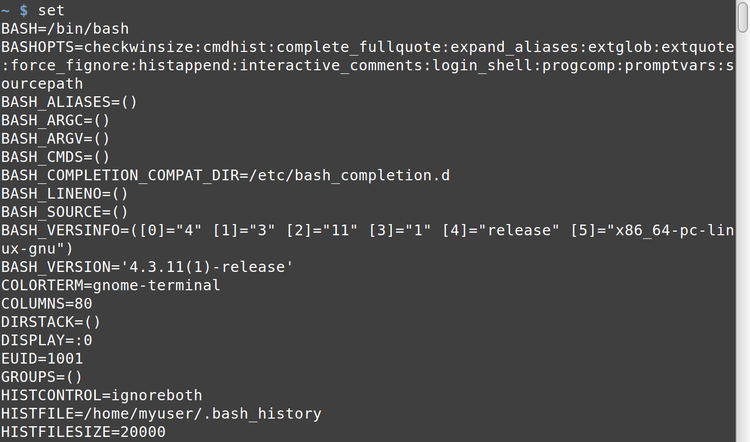
\includegraphics{./images/set.png}%
\caption{set command in bash}%
\end{figure}

\else

\begin{figure}[htbp]
\centering
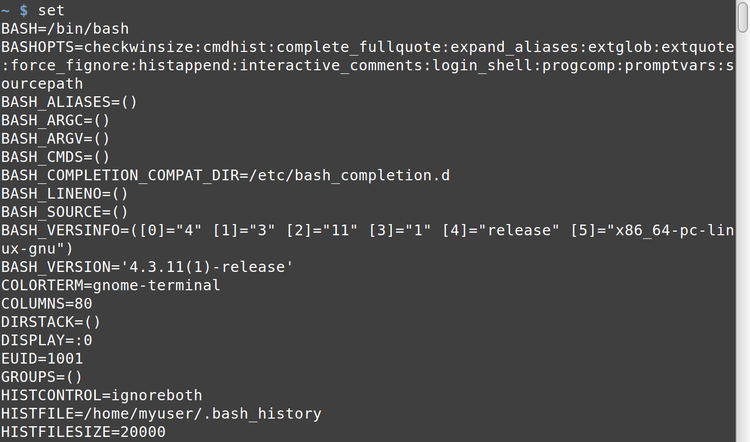
\includegraphics{./images/set.png}
\caption{set command in bash}
\end{figure}

\fi

\textbf{\emph{CMD.EXE}}

\begin{verbatim}
C:\> set
ALLUSERSPROFILE=C:\ProgramData
APPDATA=C:\Users\myuser\AppData\Roaming
CLIENTNAME=MYMACHINE
CommandPromptType=Native
CommonProgramFiles=C:\Program Files\Common Files
CommonProgramFiles(x86)=C:\Program Files (x86)\Common Files
CommonProgramW6432=C:\Program Files\Common Files
COMPUTERNAME=JCAPPDEV
ComSpec=C:\Windows\system32\cmd.exe
ExtensionSdkDir=C:\Program Files (x86)\Microsoft SDKs\Windows\v8.0\Exten...
FP_NO_HOST_CHECK=NO
Framework35Version=v3.5
...and so on...
\end{verbatim}

Similarly, the \href{http://linux.die.net/man/1/echo}{\texttt{echo}}
command can be used to show you the contents of an environment variable
(among other things):

\textbf{\emph{bash}}

\begin{verbatim}
~ $ echo $HOME
/home/myuser
\end{verbatim}

\textbf{\emph{CMD.EXE}}

\begin{verbatim}
C:\> echo %homedrive%
C:
\end{verbatim}

This example shows some valuable differences between shells, though.
Even though both have the concept of environment variables and echoing
out their contents using the ``same'' command, note that:

\begin{enumerate}
\def\labelenumi{\arabic{enumi}.}
\item
  The syntax for accessing an environment variable is
  \texttt{\$variable} in \texttt{bash} and \texttt{\%variable\%} in
  \texttt{CMD.EXE}.
\item
  \texttt{bash} is case-sensitive and so \texttt{echo \$HOME} works but
  \texttt{echo \$home} does not. \texttt{CMD.EXE} is \textbf{\emph{not}}
  case-sensitive, so either \texttt{echo \%homedrive\%} or
  \texttt{echo \%HOMEDRIVE\%} (or \texttt{EcHo \%hOmEdRiVe\%}) would
  work.
\end{enumerate}

\section{You're a Product of Your Environment
(Variables)}\label{youre-a-product-of-your-environment-variables}

It is much more common to set up environment variables to control
execution in Linux than in Windows. In fact, it is quite common to
override a given environment variable for the single execution of a
program, to the point that \texttt{bash} has built-in ``one-line''
support for it:

\begin{verbatim}
~ $ FOO=myval /home/myuser/myscript
\end{verbatim}

This sets the environment variable \texttt{FOO} to ``myval'' but only
for the duration and scope of running \texttt{myscript}.

By convention, environment variables are named all uppercase, whereas
all scripts and programs tend to be named all lowercase. Remember,
almost without exception Linux and company are case-sensitive and
Windows is not.

You can set or override multiple variables for a single command or
script execution simply by separating them with spaces:

\begin{verbatim}
~ $ FOO=myval BAR=yourval BAZ=ourvals /home/myuser/myscript
\end{verbatim}

Note that passing in values in this way does not safeguard sensitive
information from other users on the system who can see the values at
least while the script is running using the \texttt{ps -x} command.

You can also set the value of environment variables to the output of a
command using `:

\begin{verbatim}
~ $ filetype=`file --print --mime-type --no-pad --print0 otschecker.csv`

~ $ echo $filetype
otschecker.csv: text/plain
\end{verbatim}

\subsection{Who Am I?}\label{who-am-i}

When writing scripts that can be run by any user, it may be helpful to
know their user name at run-time. There are at least two different ways
to determine that. The first is via environment variables:

\begin{verbatim}
~ $ echo $USER
myuser
\end{verbatim}

The second is with a command with one of the best names, ever -
\href{http://linux.die.net/man/1/whoami}{\texttt{whoami}}:

\begin{verbatim}
~ $ whoami
myuser
\end{verbatim}

Some environments set the \texttt{\$USER} environment variable, some set
a \texttt{\$USERNAME} variable, and some like Mint set both. I think it
is better to use \texttt{whoami}, which tends to be on almost all
systems.

\section{Paths (a Part of Any Balanced
Shrubbery)}\label{paths-a-part-of-any-balanced-shrubbery}

The concept of a ``path'' for finding executables is almost identical,
and Windows lifted it from UNIX (or CP/M, which lifted it from UNIX).
You can tell how similar they are by looking at the output of the
\texttt{PATH} environment variable under \texttt{CMD.EXE} and
\texttt{bash} running under Cygwin for the same user on the same
machine:

\textbf{\emph{CMD.EXE}}

{[}Formatted for readability{]}

\begin{verbatim}
C:\> echo %path%
C:\Program Files (x86)\Microsoft Visual Studio 11.0\Common7\IDE\CommonEx...
C:\Program Files (x86)\Microsoft Visual Studio 11.0\VC\BIN\amd64;
C:\Windows\Microsoft.NET\Framework64\v4.0.30319;
C:\Windows\Microsoft.NET\Framework64\v3.5;
C:\Program Files (x86)\Microsoft Visual Studio 11.0\VC\VCPackages;
C:\Program Files (x86)\Microsoft Visual Studio 11.0\Common7\IDE;
C:\Program Files (x86)\Microsoft Visual Studio 11.0\Common7\Tools;
...and so on...
\end{verbatim}

\textbf{\emph{bash}}

{[}Formatted for readability{]}

\begin{verbatim}
~ $ echo $PATH
/usr/local/bin:/usr/bin:/bin:/usr/local/games:/usr/games
\end{verbatim}

Note the differences and similarities. Both the paths are evaluated left
to right. Both use separators between path components, a \texttt{;} for
DOS and Windows, a \texttt{:} for Linux. Both delimit their directory
names with slashes, with \texttt{\textbackslash{}} for DOS and Windows
and \texttt{/} for Linux. But Linux has no concept of a ``drive letter''
like \texttt{C:}, and instead everything is rooted in a single namespace
hierarchy starting at the root \texttt{/}. We'll be talking more about
directories in the next chapter.

\section{Open Your Shell and
Interact}\label{open-your-shell-and-interact}

The actual ``command prompt'' is when you bring up a shell in an
``interactive session'' in a terminal window. This might be from logging
into the console of a Linux VM, or starting a terminal window in a X
window manager like GNOME or KDE, or \texttt{ssh}'ing into an
interactive session of a remote machine, or even running a Cygwin
command prompt under Windows.

Command prompts allow you to work in a so-called ``REPL'' environment
(Read, Evaluate, Print, Loop). You can run a series of commands once, or
keep refining a command or commands until you get them working the way
you want, then transfer their sequence to a script file to capture it.

Real shell wizards can often show off their magic in an incredible
one-liner typed from memory with lots of obscure commands piped together
and invoked with cryptic options.

I am not a real shell wizard. See
\hyperref[HowDoYouKnowWhatYouDontKnow]{chapter 9} for how you can fake
it like I do.

\section{Getting Lazy}\label{getting-lazy}

Most modern interactive shells like \texttt{bash} and \texttt{CMD.EXE}
allow for tab expansion and command history, at least for the current
session of the shell.

Tab expansion is ``auto-complete'' for the command prompt. Let's say you
have the following files in a directory:

\begin{verbatim}
$ ls -l
total 764
-rwxrwx---+ 1 myuser mygroup  18554 Oct  9 15:01 Agenda.md
drwxrwx---+ 1 myuser mygroup      0 Oct  9 08:50 Bad and Corrupted Test
Files
drwxrwx---+ 1 myuser mygroup      0 Sep 22 15:35 CheckMD5sLog
-rw-rwxr--+ 1 myuser mygroup   1431 Oct  9 14:58 CygwinPath.txt
-rwxrwx---+ 1 myuser mygroup  22461 Oct  7 14:19 Disabled Active Directory Accounts.xlsx
-rwxrwx---+ 1 myuser mygroup  55647 Sep 18 08:31 filtered.txt
drwxrwx---+ 1 myuser mygroup      0 Sep 15 15:59 FLOCK
-rwxrwx---+ 1 myuser mygroup  11185 Feb 24  2015 GitLab Upgrade Info.txt
...and so on...
\end{verbatim}

Without tab expansion, typing out something like:

\begin{verbatim}
~ $ mv Disabled\ Active\ Directory\ Accounts.xlsx
\end{verbatim}

\ldots{}is painful. But with tab expansion, we can simply:

\begin{verbatim}
mv D^t
\end{verbatim}

\ldots{}where \texttt{\^{}t} represents hitting the \texttt{Tab} key,
and since there is only one file that starts with a ``D'' tab expansion
will fill in the rest of the file name:

\begin{verbatim}
~ $ mv Disabled\ Active\ Directory\ Accounts.xlsx
\end{verbatim}

\ldots{}and we can go about our business of finishing our command.

One place the tab completion in \texttt{bash} is different than
\texttt{CMD.EXE} is that in \texttt{bash} if you hit \texttt{Tab} and
there are multiple candidates, it will expand as far as it can and then
show you a list of files that match up to that point and allow you to
type in more characters and hit \texttt{Tab} again to complete it.
Whereas in \texttt{CMD.EXE} it will ``cycle'' between the multiple
candidates, showing you each one as the completion option in turn. Both
are useful, but each is subtly different and can give you fits when
moving between one environment and another.

\textbf{Pro Tip:} Remember, UNIX was built by people on slow, klunky
teletypes and terminals, and they hated to type! Tab expansion is your
friend and you should use it as often as possible. It gives at least
three benefits:

\begin{enumerate}
\def\labelenumi{\arabic{enumi}.}
\item
  Saves you typing.
\item
  Helps eliminate misspellings in a long file or command name.
\item
  Acts as an error checker, because if the tab doesn't expand, chances
  are you are specifying something else (the beginning path of the file)
  wrong.
\end{enumerate}

The other thing to remember about the interactive shell is command
history. Again, both \texttt{CMD.EXE} and \texttt{bash} give you command
history, but \texttt{CMD.EXE} only remembers it for the session, while
\texttt{bash} stores it in one of your hidden ``profile'' or ``dot''
files in your home directory called \texttt{.bash\_history}:

\begin{verbatim}
~ $ ls -a
.              .bash_profile  .gitignore  .minttyrc  Dropbox      Sandbox
..             .bashrc        .inputrc    .profile   fast-export  Shared
.bash_history  .gitconfig     .lesshst    .ssh       myuser      Temp
\end{verbatim}

Inside, \texttt{.bash\_history} is just a text file, with the most
recent commands at the bottom.

The \texttt{bash} shell supports a rich interactive environment for
searching for, editing and saving command history. However, the biggest
thing you need to remember to fake it is simply that the up and down
arrows work in the command prompt and bring back your recent commands so
you can update them and re-execute them.

\textbf{Note:} If you start multiple sessions under the same account,
the saved history will be of the last login to successfully write back
out \texttt{.bash\_history}.

\chapter{File Under ``Directories''}\label{file-under-directories}

\textbf{\emph{\texttt{ls}, \texttt{mv}, \texttt{cp}, \texttt{rm}
(\texttt{-rf *}), \texttt{cat},
\texttt{chmod}/\texttt{chgrp}/\texttt{chown} and everyone's favorite,
\texttt{touch}.}}

\begin{quote}
\emph{``I'm in the phone book! I'm somebody now!''} - Navin Johnson
(\emph{The Jerk})
\end{quote}

Typically in Linux we are scripting and otherwise moving around files.
The file system under the covers may be one of any number of supported
formats, including:

\begin{itemize}
\item
  \href{https://en.wikipedia.org/wiki/Ext2}{\textbf{ext2}}
\item
  \href{https://en.wikipedia.org/wiki/Ext3}{\textbf{ext3}}
\item
  \href{https://en.wikipedia.org/wiki/Ext4}{\textbf{ext4}},
\item
  \href{https://en.wikipedia.org/wiki/ReiserFS}{\textbf{ReiserFS}}
\item
  \textbf{\ldots{}and so much more!} - NTFS, FAT, etc.
\end{itemize}

Each has its strengths and weaknesses. While Linux tends to treat the
ext* file systems as preferred, it can write to a lot of file systems
and can read even more.

As mentioned above, the biggest differences between Linux and Windows is
that the Linux environments tend not to have a concept of ``drive
letters.'' Instead everything is ``mounted'' under a single hierarchy
that starts at the ``root directory'' or \texttt{/}.

\begin{verbatim}
~ $ ls /
bin   etc         lib         media  proc  sbin     sys  var
boot  home        lib64       mnt    root  selinux  tmp  vmlinuz
dev   initrd.img  lost+found  opt    run   srv      usr
\end{verbatim}

The root file system may be backed by a disk device, LUN, memory or even
the network. It will have one or more directories under it. Multiple
physical drives and network locations can be ``mounted'' virtually
anywhere, under any directory or subdirectory in the hierarchy.

\textbf{Note:} Dynamically mounted devices like USB drives and DVDs are
often mounted automatically under either a \texttt{/mnt} or
\texttt{/media} directory.

\section{Looking at Files}\label{looking-at-files}

The command to \emph{list} the contents of a directory is the
\href{http://linux.die.net/man/1/ls}{\texttt{ls}} command:

\begin{verbatim}
~ $ ls
Desktop    Downloads  FreeRDP     Music     Public  Temp       Videos
Documents  Dropbox    installrdp  Pictures  rdp     Templates
\end{verbatim}

Remember, UNIX environments think of files that start with a \texttt{.}
as ``hidden.'' If you want to see all these
\href{https://en.wikipedia.org/wiki/Hidden_file_and_hidden_directory\#Unix_and_Unix-like_environments}{``dotfiles''},
you can use \texttt{ls -a}:

\begin{verbatim}
~ $ ls -a
.              Desktop        .gksu.lock       .mozilla   .themes
..             .dmrc          .gnome2          Music      .thumbnails
.adobe         Documents      .gnome2_private  Pictures   .thunderbird
.atom          Downloads      .hugin           .pki       Videos
.bash_history  .dropbox       .ICEauthority    .profile   .wine
.bash_logout   Dropbox        .icons           .ptbt1     .Xauthority
.cache         .dropbox-dist  installrdp       Public     .xinputrc
.cinnamon      .face          .lastpass        rdp        .xsession-errors
.cmake         FreeRDP        .linuxmint       .sbd
.config        .gconf         .local           Temp
.dbus          .gimp-2.8      .macromedia      Templates
\end{verbatim}

Wow! That's a lot of dotfiles!

If you want to see some details of each file, use \texttt{ls -l}:

\begin{verbatim}
~ $ ls -l
total 92
drwxr-xr-x  2 myuser mygroup      4096 Sep  7 04:16 Desktop
drwxr-xr-x  2 myuser mygroup      4096 Oct 13 10:02 Documents
drwxr-xr-x  2 myuser mygroup      4096 Oct 14 09:45 Downloads
drwx------  8 myuser mygroup      4096 Oct 16 19:58 Dropbox
drwxr-xr-x 19 myuser mygroup      4096 Oct 12 09:48 FreeRDP
-rwxr-x---  1 myuser sambashare    883 Oct 12 11:34 installrdp
drwxr-xr-x  5 myuser mygroup      4096 Oct 16 10:47 LightTable
drwxr-xr-x  2 myuser mygroup      4096 Sep  7 04:16 Music
drwxr-xr-x  3 myuser mygroup     36864 Oct 12 17:29 Pictures
drwxr-xr-x  2 myuser mygroup      4096 Sep  7 04:16 Public
-rwxr-xr-x  1 myuser mygroup       816 Oct 15 18:00 rdp
...and so on...
\end{verbatim}

And of course parameters can be combined, as with the two above:

\begin{verbatim}
~ $ ls -al
total 344
drwxr-xr-x 40 myuser mygroup      4096 Oct 17 07:14 .
drwxr-xr-x  3 root   root         4096 Sep  7 04:09 ..
drwx------  3 myuser mygroup      4096 Sep  7 09:33 .adobe
drwxr-xr-x  5 myuser mygroup      4096 Oct 12 15:48 .atom
-rw-------  1 myuser mygroup      6428 Oct 17 06:11 .bash_history
-rw-r--r--  1 myuser mygroup       220 Sep  7 04:09 .bash_logout
drwx------ 18 myuser mygroup      4096 Oct 13 07:31 .cache
drwxr-xr-x  5 myuser mygroup      4096 Oct 16 19:57 .cinnamon
drwxr-xr-x  3 myuser mygroup      4096 Oct 12 09:45 .cmake
drwxr-xr-x 26 myuser mygroup      4096 Oct 15 10:23 .config
drwx------  3 myuser mygroup      4096 Sep  7 04:16 .dbus
...and so on...
\end{verbatim}

\section{A Brief Detour Around
Parameters}\label{a-brief-detour-around-parameters}

In \texttt{bash} and many Linux commands in general, there are old,
``short'' (terse) parameter names, like \texttt{ls -a}, and newer,
longer, descriptive parameter names like \texttt{ls -{}-all} that mean
the same thing. It is typically good to use the shorter version during
interactive sessions and testing, but I prefer long parameter names in
scripts, because when I come back and look at it in two years, I may not
remember what \texttt{rm -rf *} means (in the ``UNIX'' world it means
you're toast if you run it in the wrong directory by mistake), thus
\texttt{rm -{}-recursive -{}-force *} seems a bit more ``intuitive.''

\begin{quote}
\textbf{\emph{The behind you save in the future by describing things
well today may well be your own.}} - me
\end{quote}

The older style parameters are typically preceded by a single hyphen
``switch'' character:

\begin{verbatim}
~ $ ls -r
\end{verbatim}

Or even no ``switch'' character at all, as with \texttt{xvf}
(e\textbf{\emph{X}}tract, \textbf{\emph{V}}erbose, input
\textbf{\emph{F}}ile name) in the following:

\begin{verbatim}
~ $ tar xvf backup.tar
\end{verbatim}

The newer ``GNU-style'' parameters are preceded by two hyphens and
usually are quite ``verbose'':

\begin{verbatim}
~ $ ls --recursive --almost-all --ignore-backups
\end{verbatim}

Again, it is \textbf{\emph{highly recommended}} that you take the time
to use the GNU-style parameters in scripts as self-documenting code.

\section{More Poking at Files}\label{more-poking-at-files}

If we suspect the file is a text file, we can echo it to the console
with the \href{http://linux.die.net/man/1/cat}{\texttt{cat}}
(\emph{concatenate}) command:

\begin{verbatim}
~ $ cat installrdp 
#!/bin/bash
sudo apt-get -y install git
cd ~
git clone git://github.com/FreeRDP/FreeRDP.git
cd FreeRDP
sudo apt-get -y install build-essential git-core cmake libssl-dev \
  libx11-dev libxext-dev libxinerama-dev libxcursor-dev libxdamage-dev \
  libxv-dev libxkbfile-dev libasound2-dev libcups2-dev   libxml2 \
  libxml2-dev libxrandr-dev libgstreamer0.10-dev \
  libgstreamer-plugins-base0.10-dev libxi-dev \
  libgstreamer-plugins-base1.0-dev libavutil-dev libavcodec-dev \
  libcunit1-dev libdirectfb-dev xmlto doxygen libxtst-dev
cmake -DCMAKE_BUILD_TYPE=Debug -DWITH_SSE2=ON .
make
sudo make install
sudo echo "/usr/local/lib/freerdp" > /etc/ld.so.conf.d/freerdp.conf
sudo echo "/usr/local/lib64/freerdp" >> /etc/ld.so.conf.d/freerdp.conf
sudo echo "/usr/local/lib" >> /etc/ld.so.conf.d/freerdp.conf
sudo ldconfig
which xfreerdp
xfreerdp --version
\end{verbatim}

We can determine from the above that \texttt{installrdp} is a
\texttt{bash} shell script that looks to install and configure
\href{https://github.com/FreeRDP/FreeRDP}{FreeRDP} on a Debian-style
system:

\begin{enumerate}
\def\labelenumi{\arabic{enumi}.}
\item
  \textbf{\texttt{apt-get}} - Debian-style package manager.
\item
  \textbf{\texttt{git clone}} - cloning package from
  \href{http://github.com}{GitHub}.
\item
  \textbf{\texttt{cmake}} and \textbf{\texttt{make}} - configuring and
  building software from source.
\end{enumerate}

A better way to display a longer file is to use the
\href{http://linux.die.net/man/1/less}{\texttt{less}} command (which is
a derivative of the original
\href{http://linux.die.net/man/1/more}{\texttt{more}}, hence the name).
\texttt{less} is a paginator, where the \texttt{Space},
\texttt{Page Down} or down arrow keys scroll down and the
\texttt{Page Up} or up arrow keys scrolls up. \texttt{Q} quits.

\textbf{Note:} The \texttt{vi} search (\texttt{/}, \texttt{?},
\texttt{n} and \texttt{p}) and navigation (\texttt{G}, \texttt{0}) keys
work within \texttt{less}, too. In general \texttt{less} is a great
lightweight way to motor around in a text file without editing it.

We can also look at just the end or \emph{tail} of a file (often the
most interesting when looking at log files and troubleshooting a current
problem) with the \href{http://linux.die.net/man/1/tail}{\texttt{tail}}
command. To show the last 10 lines of the kernel \texttt{dmesg} log:

\begin{verbatim}
# tail dmesg
[    2.774931] loop: module loaded
[    3.349880] eth0: intr type 3, mode 0, 3 vectors allocated
[    3.351331] eth0: NIC Link is Up 10000 Mbps
[    3.422647] RPC: Registered named UNIX socket transport module.
[    3.422649] RPC: Registered udp transport module.
[    3.422650] RPC: Registered tcp transport module.
[    3.422651] RPC: Registered tcp NFSv4.1 backchannel transport module.
[    3.432437] FS-Cache: Loaded
[    3.443980] FS-Cache: Netfs 'nfs' registered for caching
[    3.449794] Installing knfsd (copyright (C) 1996 okir@monad.swb.de).
\end{verbatim}

To show the last 20 lines:

\begin{verbatim}
# tail -n 20 dmesg
[    2.317838] [drm] Fifo max 0x00040000 min 0x00001000 cap 0x0000077f
[    2.318843] [drm] Supports vblank timestamp caching Rev 1 (10.10.2010).
[    2.318845] [drm] No driver support for vblank timestamp query.
[    2.318914] [drm] Screen objects system initialized
[    2.318917] [drm] Detected no device 3D availability.
[    2.323011] [drm] Initialized vmwgfx 2.4.0 20120209 for 0000:00:0f.0 ...
[    2.486733] input: ImPS/2 Generic Wheel Mouse as /devices/platform/i8...
[    2.655694] Adding 4191228k swap on /dev/sda5.  Priority:-1 extents:1...
[    2.666714] EXT4-fs (sda1): re-mounted. Opts: (null)
[    2.754699] EXT4-fs (sda1): re-mounted. Opts: errors=remount-ro
[    2.774931] loop: module loaded
[    3.349880] eth0: intr type 3, mode 0, 3 vectors allocated
[    3.351331] eth0: NIC Link is Up 10000 Mbps
[    3.422647] RPC: Registered named UNIX socket transport module.
[    3.422649] RPC: Registered udp transport module.
[    3.422650] RPC: Registered tcp transport module.
[    3.422651] RPC: Registered tcp NFSv4.1 backchannel transport module.
[    3.432437] FS-Cache: Loaded
[    3.443980] FS-Cache: Netfs 'nfs' registered for caching
[    3.449794] Installing knfsd (copyright (C) 1996 okir@monad.swb.de).
\end{verbatim}

You can also use \texttt{tail} to \emph{follow} an open file and
continuously display any new output at the end, which is useful for
monitoring log files in real time:

\begin{verbatim}
# tail -f dmesg
[    2.774931] loop: module loaded
[    3.349880] eth0: intr type 3, mode 0, 3 vectors allocated
[    3.351331] eth0: NIC Link is Up 10000 Mbps
[    3.422647] RPC: Registered named UNIX socket transport module.
[    3.422649] RPC: Registered udp transport module.
[    3.422650] RPC: Registered tcp transport module.
[    3.422651] RPC: Registered tcp NFSv4.1 backchannel transport module.
[    3.432437] FS-Cache: Loaded
[    3.443980] FS-Cache: Netfs 'nfs' registered for caching
[    3.449794] Installing knfsd (copyright (C) 1996 okir@monad.swb.de).
...new lines will appear here over time...
\end{verbatim}

If we know nothing about a \emph{file}, we can use the
\href{http://linux.die.net/man/1/file}{\texttt{file}} command to help us
guess:

\begin{verbatim}
~ $ file installrdp 
installrdp: Bourne-Again shell script, ASCII text executable
\end{verbatim}

That's straightforward enough! The \texttt{file} command isn't always
100\% accurate, but it is pretty good and uses an interesting set of
heuristics and a text file ``database'' of
\href{http://linux.die.net/man/5/magic}{``magic'' number definitions} to
define how it figures out what type of file it is examining.

\textbf{Remember:} File extensions have no real meaning per se in Linux
(although some are used, especially for media and document formats), so
a file name with no extension like \texttt{installrdp} is perfectly
valid. Hence the utility of the \texttt{file} command.

\section{Sorting Things Out}\label{sorting-things-out}

The \href{http://linux.die.net/man/1/sort}{\texttt{sort}} command can be
used to not just \emph{sort} files, but also to merge them and remove
duplicates.

Let's say we have three files:

\begin{verbatim}
~ $ ls
ElevatorTrucks  FarmCombines  FarmTractors
\end{verbatim}

Here are the contents of each:

\begin{verbatim}
~ $ cat ElevatorTrucks
Truck   brakes  200
Truck   tires   400
Truck   tires   400
Truck   tires   400
Truck   winch   100

~ $ cat FarmCombines
Combine motor   1500
Combine brakes  400
Combine tires   2500

~ $ cat FarmTractors
Tractor motor   1000
Tractor brakes  300
Tractor tires   2000
\end{verbatim}

But what if we wanted to process all the lines in all the files in a
single alphabetical order? Just redirecting the files into a program
won't do it, because the file names will be sorted by the shell and the
lines will be processed in file name order, not the ultimate sorted
order of all the file contents:

\begin{verbatim}
~ $ cat *
Truck   brakes  200
Truck   tires   400
Truck   tires   400
Truck   tires   400
Truck   winch   100
Combine motor   1500
Combine brakes  400
Combine tires   2500
Tractor motor   1000
Tractor brakes  300
Tractor tires   2000
\end{verbatim}

The \texttt{sort} command to the rescue!

\begin{verbatim}
~ $ sort *
Combine brakes  400
Combine motor   1500
Combine tires   2500
Tractor brakes  300
Tractor motor   1000
Tractor tires   2000
Truck   brakes  200
Truck   tires   400
Truck   tires   400
Truck   tires   400
Truck   winch   100
\end{verbatim}

What if we want to sort by the parts column? Well, it is the second
``key'' field delimited by whitespace, so:

\begin{verbatim}
~ $ sort -k 2 *
Truck   brakes  200
Tractor brakes  300
Combine brakes  400
Tractor motor   1000
Combine motor   1500
Tractor tires   2000
Combine tires   2500
Truck   tires   400
Truck   tires   400
Truck   tires   400
Truck   winch   100
\end{verbatim}

What about by the third column, the amount?

\begin{verbatim}
~ $ sort -k 3 *
Truck   winch   100
Tractor motor   1000
Combine motor   1500
Truck   brakes  200
Tractor tires   2000
Combine tires   2500
Tractor brakes  300
Combine brakes  400
Truck   tires   400
Truck   tires   400
Truck   tires   400
\end{verbatim}

That's not what we expected because it is sorting numbers
alphabetically. Let's fix that by telling it to sort numerically:

\begin{verbatim}
~ $ sort -k 3 -n *
Truck   winch   100
Truck   brakes  200
Tractor brakes  300
Combine brakes  400
Truck   tires   400
Truck   tires   400
Truck   tires   400
Tractor motor   1000
Combine motor   1500
Tractor tires   2000
Combine tires   2500
\end{verbatim}

Maybe we care about the top three most expensive items. We haven't
talked about pipes yet, but check this out:

\begin{verbatim}
~ $ sort -k 3 -n * | tail -n 3
Combine motor   1500
Tractor tires   2000
Combine tires   2500
\end{verbatim}

Finally, what if we want only unique rows?

\begin{verbatim}
~ $ sort -k 3 -n -u *
Truck   winch   100
Truck   brakes  200
Tractor brakes  300
Truck   tires   400
Tractor motor   1000
Combine motor   1500
Tractor tires   2000
Combine tires   2500
\end{verbatim}

Just to reinforce long parameters, the last example is equivalent to:

\begin{verbatim}
~ $ sort --key 3 --numeric-sort --unique *
Truck   winch   100
Truck   brakes  200
Tractor brakes  300
Truck   tires   400
Tractor motor   1000
Combine motor   1500
Tractor tires   2000
Combine tires   2500
\end{verbatim}

\section{Rearranging Deck Chairs}\label{rearranging-deck-chairs}

We can copy, move or rename (same thing) and delete files and
directories. To \emph{copy}, simply use the
\href{http://linux.die.net/man/1/cp}{\texttt{cp}} command:

\begin{verbatim}
~ $ cp diary.txt diary.bak
\end{verbatim}

You can copy entire directories recursively:

\begin{verbatim}
~ $ cp -r thisdir thatdir
\end{verbatim}

Or, if we want to be self-documenting in a script, we can use those long
parameter names:

\begin{verbatim}
~ $ cp --recursive thisdir thatdir
\end{verbatim}

To \emph{move} use \href{http://linux.die.net/man/1/mv}{\texttt{mv}}:

\begin{verbatim}
~ $ mv thismonth.log lastmonth.log
\end{verbatim}

\textbf{Note:} There is no semantic difference between ``move'' and
``rename.'' However, there are some really cool renaming scenarios that
the \href{http://linux.die.net/man/1/rename}{\texttt{rename}} command
can take care of beyond \texttt{mv}, like renaming all file extensions
from \texttt{.htm} to \texttt{.html}.

\section{Making Files Disappear}\label{making-files-disappear}

To delete or \emph{remove} a file you use
\href{http://linux.die.net/man/1/rm}{\texttt{rm}}:

\begin{verbatim}
~ $ rm desktop.ini
\end{verbatim}

\textbf{Pro Tip:} There is no ``Are you sure?'' prompt when removing a
single file specified with no wildcards, or even all files with a
wildcard, and there is no ``Recycle Bin'' or ``Trash Can'' when working
from the command prompt, so be careful!

This kind of scenario can happen \textbf{\emph{way}} too often, even to
experienced system administrators (note the space between \texttt{*} and
\texttt{.bak}):

\begin{verbatim}
~ $ cd MyDissertation

~ $ ls
Citations.bak  Citations.doc  Dissertation.bak  Dissertation.doc  Notes.doc

~ $ rm * .bak
rm: cannot remove ‘.bak’: No such file or directory

~ $ ls
\end{verbatim}

So, in order, our hapless user:

\begin{enumerate}
\def\labelenumi{\arabic{enumi}.}
\item
  Changed to directory \texttt{MyDissertation}.
\item
  Listed the directory contents with \texttt{ls}, saw the combination of
  \texttt{.doc} and \texttt{.bak} files.
\item
  Decided to delete the \texttt{.bak} files with \texttt{rm}, but
  accidentally typed in a space between the wildcard \texttt{*} and the
  \texttt{.bak}. Note ominous warning message.
\item
  Presto! \texttt{ls} shows \textbf{\emph{everything}} is gone, not just
  the backup files! Yay! The user's day's priorities just got rearranged
  as they go hunting for another backup of their dissertation.
\end{enumerate}

So be careful out there! This is an example where tab completion can be
an extra error check. Or a lot of times I use command history in these
cases by changing the \texttt{ls} to look for just the files I want to
delete:

\begin{verbatim}
~ $ ls *.bak
Citations.bak  Dissertation.bak
\end{verbatim}

Then using the ``up arrow'' to bring back up the \texttt{ls} command and
changing \texttt{ls} to \texttt{rm} and re-executing it. Safer that way.

\section{Touch Me}\label{touch-me}

We just learned how to make a file disappear. We can also make a file
magically appear, just by
\href{http://linux.die.net/man/1/touch}{\texttt{touch}}:

\begin{verbatim}
~ $ touch NewEmptyDissertation.doc

~ $ ls -l
total 0
-rw-rwxr--+ 1 myuser mygroup 0 Oct 19 14:12 NewEmptyDissertation.doc
\end{verbatim}

Notice the newly created file is zero bytes long.

Interestingly enough, we can also use touch just to update the ``last
modified date'' of an existing file, as you can see in time change in
the following listing after running \texttt{touch} on the same file
again:

\begin{verbatim}
~ $ touch NewEmptyDissertation.doc

~ $ ls -l
total 0
-rw-rwxr--+ 1 myuser mygroup 0 Oct 19 14:14 NewEmptyDissertation.doc
\end{verbatim}

It can be useful (but also distressing from a forensics point of view)
to sometimes set the last modified date of a file to a specific date and
time, which \texttt{touch} also allows you to do, in this case to the
night before Christmas:

\begin{verbatim}
~ $ touch -t 201412242300 NewEmptyDissertation.doc

~ $ ls -l
total 0
-rw-rwxr--+ 1 myuser mygroup 0 Dec 24  2014 NewEmptyDissertation.doc
\end{verbatim}

To \emph{make a directory} you use
\href{http://linux.die.net/man/1/mkdir}{\texttt{mkdir}}:

\begin{verbatim}
~ $ mkdir Bar

~ $ ls
Bar
\end{verbatim}

Typically you need to create all intervening directories before creating
a ``child'' directory:

\begin{verbatim}
~ $ mkdir Xyzzy/Something
mkdir: cannot create directory ‘Xyzzy/Something’: No such file or directory
\end{verbatim}

But of course you can override that behavior:

\begin{verbatim}
~ $ mkdir --parents Xyzzy/Something

~ $ ls
Bar  Xyzzy

~ $ ls Xyzzy
Something
\end{verbatim}

\section{Navigating Through Life}\label{navigating-through-life}

Ever notice that ``life'' is an anagram for ``file''? Spooky, eh?

Given that the UNIX-style file systems are hierarchical in nature they
are similar to navigate as with \texttt{CMD.EXE}. The biggest difference
is the absense of drive letter and the direction of the slashes.

To \emph{change directories}, simply use
\href{http://linux.die.net/man/1/cd}{\texttt{cd}} much like in Windows:

\begin{verbatim}
~ $ cd /etc

~ $ pwd
/etc
\end{verbatim}

\href{http://linux.die.net/man/1/pwd}{\texttt{pwd}} simply \emph{prints
the working (current) directory}.

In Linux, users can have ``home'' directories (similar to Windows
profiles), typically located under \texttt{/home/username} for normal
users and \texttt{/root} for the ``root'' id. To change to a user's
``home'' directory, simply use \texttt{cd}:

\begin{verbatim}
~ $ cd

~ $ pwd
/home/myuser
\end{verbatim}

The tilde (\texttt{\textasciitilde{}}) character is an alias for the
current user's home directory. The following example is equivalent to
above:

\begin{verbatim}
~ $ cd ~

~ $ pwd
/home/myuser
\end{verbatim}

More useful is that the tilde can be combined with a user name to
specify the home directory of \textbf{\emph{another}} user:

\begin{verbatim}
~ $ cd ~git

~ $ pwd
/home/git
\end{verbatim}

\textbf{Note:} The above assumes you have permissions to \texttt{cd}
into \texttt{/home/git}. See the section on file permissions for more
info.

In addition, you need to know the difference between ``absolute'' and
``relative'' paths:

\begin{itemize}
\item
  \textbf{Absolute path} - \textbf{\emph{always}} ``goes through'' or
  specifies the ``root'' (\texttt{/}) directory, e.g. \texttt{cd /etc}.
\item
  \textbf{Relative path} - does \textbf{\emph{not}} specify the root
  directory, expects to start the navigation at the current directory
  with all path components existing from there, e.g.,
  \texttt{cd Dissertations}.
\end{itemize}

Windows inherited the concept of \texttt{.} for the current directory
and \texttt{..} for the parent directory directly from UNIX. Consider
the following examples that combine all of the above about relative
paths and see if it all makes sense:

\begin{verbatim}
~ $ mkdir Bar Baz

~ $ ls
Bar  Baz

~ $ cd Bar

~ $ touch a b c

~ $ ls
a  b  c

~ $ cd ../Baz

~ $ ls

~ $ touch d e f

~ $ ls
d  e  f

~ $ ls ..
Bar  Baz

~ $ ls ../Bar
a  b  c
\end{verbatim}

Did you notice how both \texttt{mkdir} and \texttt{touch} allow for
specifying multiple directory and file names in the same command?

\section{May I?}\label{may-i}

Most UNIX-style file systems come with a set of nine permissions that
can be thought of as a ``grid'' of 3x3 showing ``who has what?'' The
``who'' is ``UGO'':

\begin{itemize}
\item
  \textbf{User} - the user that is the ``owner'' of the file or
  directory.
\item
  \textbf{Group} - the group that is the ``owner'' of the file or
  directory.
\item
  \textbf{Other} - everyone else.
\end{itemize}

The ``what'' is:

\begin{itemize}
\item
  \textbf{Read}
\item
  \textbf{Write}
\item
  \textbf{Execute} - for files, for directories this means ``navigate''
  or ``list contents''.
\end{itemize}

The combination of ``who has what?'' is usually shown in detailed
directory listings by a set of ten characters, with the first one
determining whether an entry is a directory or a file:

\begin{verbatim}
# ls -l /etc
total 844
drwxr-xr-x 3 root root    4096 Feb 25  2015 acpi
-rw-r--r-- 1 root root    2981 Apr 23  2014 adduser.conf
-rw-r--r-- 1 root root      45 Jul  9 08:46 adjtime
-rw-r--r-- 2 root root     621 May 22  2014 aliases
-rw-r--r-- 1 root root   12288 May 22  2014 aliases.db
drwxr-xr-x 2 root root   20480 Feb 25  2015 alternatives
-rw-r--r-- 1 root root    4185 Dec 28  2011 analog.cfg
drwxr-xr-x 7 root root    4096 Feb 25  2015 apache2
drwxr-xr-x 6 root root    4096 Feb 25  2015 apt
-rw-r----- 1 root daemon   144 Jun  9  2012 at.deny
-rw-r--r-- 1 root root    1895 Dec 29  2012 bash.bashrc
-rw-r--r-- 1 root root      45 Jun 17  2012 bash_completion
drwxr-xr-x 2 root root    4096 Feb 25  2015 bash_completion.d
...and so on...
\end{verbatim}

In the above, for example, we can see that the user \texttt{root} owns
the file \texttt{at.deny} while the \texttt{daemon} group is the primary
group for it. \texttt{root} can both read and write the file
(\texttt{rw-}) while any user in the \texttt{daemon} group can only
reade it (\texttt{r-{}-}). No other id will have any access to the file
at all (\texttt{-{}-{}-}).

Similarly we see that \texttt{acpi} is a directory (\texttt{d}) that can
be read, written (new files created) and listed by \texttt{root}
(\texttt{rwx}), and read and listed by the group \texttt{root} and all
other ids (\texttt{r-xr-x}).

If we look in \texttt{/etc/init.d} where many services store their
startup scripts we see:

\begin{verbatim}
# ls -l /etc/init.d
total 332
-rwxr-xr-x 1 root root  2227 Apr 15  2013 acpid
-rwxr-xr-x 1 root root  7820 Jan 31  2014 apache2
-rwxr-xr-x 1 root root  1071 Jun 25  2011 atd
-rwxr-xr-x 1 root root  1276 Oct 15  2012 bootlogs
-rwxr-xr-x 1 root root  1281 Jul 14  2013 bootmisc.sh
-rwxr-xr-x 1 root root  3816 Jul 14  2013 checkfs.sh
-rwxr-xr-x 1 root root  1099 Jul 14  2013 checkroot-bootclean.sh
-rwxr-xr-x 1 root root  9673 Jul 14  2013 checkroot.sh
-rwxr-xr-x 1 root root  1379 Dec  8  2011 console-setup
-rwxr-xr-x 1 root root  3033 Jul  3  2012 cron
-rwxr-xr-x 1 root root  2813 Feb  5  2015 dbus
-rwxr-xr-x 1 root root  6435 Jan  2  2013 exim4
...and so on...
\end{verbatim}

In this case all the scripts are readable, writable and executable
(\texttt{rwx}) by the \texttt{root} user, and readable and executable by
the \texttt{root} group and all other users (\texttt{r-xr-x}).

To \emph{change} the \emph{owning} user of a file or directory (assuming
you have permissions to do so), use the
\href{http://linux.die.net/man/1/chown}{\texttt{chown}} command:

\begin{verbatim}
# ls -l
total 4
-rwxr--r-- 1 root root 17 Oct 20 10:07 foo

# chown git foo

# ls -l
total 4
-rwxr--r-- 1 git root 17 Oct 20 10:07 foo
\end{verbatim}

To \emph{change} the primary \emph{group}, use the
\href{http://linux.die.net/man/1/chgrp}{\texttt{chgrp}} command:

\begin{verbatim}
# chgrp git foo

# ls -l
total 4
-rwxr--r-- 1 git git 17 Oct 20 10:07 foo
\end{verbatim}

To \emph{change} the various permissions or \emph{mode} bits, you use
the \href{http://linux.die.net/man/1/chmod}{\texttt{chmod}} command. It
uses mnemonics of ``ugo'' for (owning) user, group and ``other,''
respectively. It also uses mnemonics of ``rwx'' for read, write and
execute, and \texttt{+} to add a permission and \texttt{-} to remove it.
For example, to add execute permission for the group and remove read
permission for ``other'':

\begin{verbatim}
# chmod g+x,o-r foo

# ls -l
total 4
-rwxr-x--- 1 git git 17 Oct 20 10:07 foo
\end{verbatim}

\textbf{Pro Tip:} To look like an old hand UNIX hacker, you can also
convert any set of ``rwx'' permissions into an octal number from 0 (no
permissions) to 7 (all permissions). It helps to think of the three
permissions as ``binary places'':

\begin{itemize}
\itemsep1pt\parskip0pt\parsep0pt
\item
  \textbf{r} - 2\^{}2 = 4
\item
  \textbf{w} - 2\^{}1 = 2
\item
  \textbf{x} - 2\^{}0 = 1
\item
  \textbf{-} - 0
\end{itemize}

Some examples:

\begin{itemize}
\itemsep1pt\parskip0pt\parsep0pt
\item
  \textbf{---} - 0 + 0 + 0 = 0
\item
  \textbf{r--} - 2\^{}2 + 0 + 0 = 4
\item
  \textbf{r-x} - 2\^{}2 + 0 + 2\^{}0 = 5
\item
  \textbf{rw-} - 2\^{}2 + 2\^{}1 + 0 = 6
\item
  \textbf{rwx} - 2\^{}2 + 2\^{}1 + 2\^{}0 = 7
\end{itemize}

Now to use octal with \texttt{chmod}, we think of the overall result we
want for a file. For example, if we want the \texttt{foo} file to be
readable, writable and executable by both its owning user and group, and
not accessible at all by anyone else, we could use:

\begin{verbatim}
# chmod u+rwx,g+rwx,o- foo

# ls -l
total 4
-rwxrwx--- 1 git git 17 Oct 20 10:07 foo
\end{verbatim}

Or we could simply convert those permissions into octal in our head and:

\begin{verbatim}
# chmod 770 foo

# ls -l
total 4
-rwxrwx--- 1 git git 17 Oct 20 10:07 foo
\end{verbatim}

Now you know the answer to that ``How will we ever use octal in real
life?'' question you asked in school!

\textbf{Note:} For a script or executable file to be allowed to run, it
\textbf{\emph{must}} be marked as executable for one of the user, group
or other entries. The following should be insightful:

\begin{verbatim}
# echo "echo Hello world" > foo

# ls -l
total 4
-rw-r--r-- 1 root root 17 Oct 20 10:07 foo

# ./foo
-bash: ./foo: Permission denied

# chmod u+x foo

# ls -l
total 4
-rwxr--r-- 1 root root 17 Oct 20 10:07 foo

# ./foo
Hello world
\end{verbatim}

\section{``I'll Send You a Tar Ball''}\label{ill-send-you-a-tar-ball}

In the Windows world, we are used to compressing and sending directories
around as \texttt{.zip} files. In Linux you can also deal with
\texttt{.zip} files, although they don't tend to be the most common,
using the \href{http://linux.die.net/man/1/zip}{\texttt{zip}} and
\href{http://linux.die.net/man/1/unzip}{\texttt{unzip}} commands:

\begin{verbatim}
~ $ mkdir foo

~ $ cd foo

~ $ touch a b c

~ $ mkdir d

~ $ touch d/e

~ $ cd ..

~ $ zip -r foo foo
updating: foo/ (stored 0%)
  adding: foo/c (stored 0%)
  adding: foo/b (stored 0%)
  adding: foo/d/ (stored 0%)
  adding: foo/d/e (stored 0%)
  adding: foo/a (stored 0%)

~ $ ls -l foo.zip
-rw-r--r-- 1 myuser mygroup 854 Oct 24 15:56 foo.zip

~ $ unzip foo
Archive:  foo.zip
replace foo/c? [y]es, [n]o, [A]ll, [N]one, [r]ename: A
 extracting: foo/c                   
 extracting: foo/b                   
 extracting: foo/d/e                 
 extracting: foo/a                   
\end{verbatim}

Not too exciting, but you get the drift. There is typically support for
other compression algorithms, too, using
\href{http://linux.die.net/man/1/bzip2}{\texttt{bzip2}} and
\href{http://linux.die.net/man/1/7z}{\texttt{7z}} (7-zip) commands.

However, the ``native'' way to ``archive'' a directory's contents in
``UNIX'' is with \href{http://linux.die.net/man/1/tar}{\texttt{tar}},
which is so old that \texttt{tar} stands for ``tape archive.'' Its
purpose is to take virtually any directory structure and create a single
output ``stream'' or file of it. That is then typically ran through a
compression command and the result is called a ``tarball'':

\begin{verbatim}
~ $ tar cvf foo.tar foo/*
foo/a
foo/b
foo/c
foo/d/
foo/d/e

~ $ ls -l foo.tar
-rw-r--r-- 1 myuser mygroup 10240 Oct 24 16:14 foo.tar

~ $ gzip foo.tar

~ $ ls -l foo.tar.gz 
-rw-r--r-- 1 myuser mygroup 187 Oct 24 16:14 foo.tar.gz
\end{verbatim}

In the \texttt{tar} command above, the parameters are \texttt{c} (create
a new archive), \texttt{v} (turn on ``verbose'' output) and \texttt{f}
followed by the file name of the new \texttt{.tar} file.

\textbf{Note:} \texttt{tar} supports POSIX-style parameters
(\texttt{-c}), GNU-style (\texttt{-{}-create}), and the old BSD-style
(\texttt{c} with no hyphens at all), as shown in these examples. So both
of the following are also equivalent to the above:

\begin{verbatim}
~ $ tar -c -v -f foo.tar foo/*

~ $ tar --create --verbose --file=foo.tar foo/*
\end{verbatim}

The use of compression commands along with \texttt{tar} is so prevalent
that they've been built into \texttt{tar} itself now as optional
parameters:

\begin{verbatim}
~ $ tar cvzf foo.tgz foo
foo/
foo/c
foo/b
foo/d/
foo/d/e
foo/a

~ $ ls -l foo.tgz
-rw-r--r-- 1 myuser mygroup 191 Oct 24 16:19 foo.tgz
\end{verbatim}

In this case the \texttt{z} parameter says to use \texttt{gzip}
compression, and the \texttt{.tgz} file suffix means basically ``tarred
and gzipped'', or the equivalent to \texttt{.tar.gz} in the first
example.

\texttt{tar} is used to both create and read \texttt{.tar} files. So to
extract something like the above, you can change the create (\texttt{c})
parameter to extract (\texttt{x}), like this:

\begin{verbatim}
~ $ tar xvf foo.tgz
foo/
foo/c
foo/b
foo/d/
foo/d/e
foo/a
\end{verbatim}

\section{Let's Link Up!}\label{lets-link-up}

In Windows there are ``shortcuts,'' which are simply special files that
the OS knows to interpret as ``go open this other file over there.''
There are also ``hard links'' that allow to different directory entries
\emph{in the same file system} to point to the same physical file.

UNIX file systems also have both these types of links (which isn't
surprising, given that Microsoft got the ideas from UNIX). A ``soft
link'' is equivalent to a Windows shortcut, and can point to a file or a
directory, and can point to anything on any mounted file system:

\begin{verbatim}
~ $ ls -l
total 4
-rw-r--r-- 1 myuser mygroup    0 Oct 24 15:53 a
-rw-r--r-- 1 myuser mygroup    0 Oct 24 15:53 b
-rw-r--r-- 1 myuser mygroup    0 Oct 24 15:53 c
drwxr-xr-x 2 myuser mygroup 4096 Oct 24 16:00 d

~ $ cd d

~ $ pwd
/tmp/foo/d

~ $ cd ..

~ $ ln -s a MyThesis.doc

~ $ ln -s d Dee

~ $ ls -l
total 4
-rw-r--r-- 1 myuser mygroup    0 Oct 24 15:53 a
-rw-r--r-- 1 myuser mygroup    0 Oct 24 15:53 b
-rw-r--r-- 1 myuser mygroup    0 Oct 24 15:53 c
drwxr-xr-x 2 myuser mygroup 4096 Oct 24 16:00 d
lrwxrwxrwx 1 myuser mygroup    1 Oct 24 16:40 Dee -> d
lrwxrwxrwx 1 myuser mygroup    1 Oct 24 16:40 MyThesis.doc -> a

~ $ cd Dee

~ $ pwd
/tmp/foo/Dee
\end{verbatim}

The things to notice about this example:

\begin{enumerate}
\def\labelenumi{\arabic{enumi}.}
\item
  The \texttt{-s} parameter indicates ``create a \emph{soft} link.''
\item
  Instead of a \texttt{-} or \texttt{d}, a soft link is shown in a
  \texttt{ls} listing as \texttt{l} regardless of whether the target is
  a file or directory. This is because a soft link doesn't ``know''
  \textbf{\emph{what}} the target is - it is just a file with a name in
  a directory pointing to another location. \textbf{\emph{What}} that
  location is will be determine after the link is traversed.
\end{enumerate}

A ``hard link'' is a bit different. It can only be made between files
and the two files must be on the same file system. That is because hard
links are actually directory entries (as opposed to files in
directories) that point to the same
\href{https://en.wikipedia.org/wiki/Inode}{``inode''} on disk. From
within a single directory it is impossible to tell if there are other
directories with pointers to the same files (inodes) on disk.

\begin{verbatim}
~ $ ls
a  b  c  d  Dee  MyThesis.doc

~ $ ln b B

~ $ cd d

~ $ ln ../b .

~ $ ls -l
total 0
-rw-r--r-- 3 myuser mygroup 0 Oct 24 15:53 b
-rw-r--r-- 1 myuser mygroup 0 Oct 24 15:54 e

~ $ cd ..

~ $ ls -l
total 4
-rw-r--r-- 1 myuser mygroup    0 Oct 24 15:53 a
-rw-r--r-- 3 myuser mygroup    0 Oct 24 15:53 b
-rw-r--r-- 3 myuser mygroup    0 Oct 24 15:53 B
-rw-r--r-- 1 myuser mygroup    0 Oct 24 15:53 c
drwxr-xr-x 2 myuser mygroup 4096 Oct 24 16:49 d
lrwxrwxrwx 1 myuser mygroup    1 Oct 24 16:40 Dee -> d
lrwxrwxrwx 1 myuser mygroup    1 Oct 24 16:40 MyThesis.doc -> a
\end{verbatim}

The ``net net'' of all the above is that now \texttt{b}, \texttt{B} and
\texttt{d/b} all point to exactly the same inode, or disk location,
i.e., the exact same physical file.

\subsection{I Said ``Go Away!'', Dammit!}\label{i-said-go-away-dammit}

So what can possibly go wrong with links? With soft links the answer is
easy - the ``remote'' location being pointed to goes away or is renamed:

\begin{verbatim}
~ $ ls -l
total 4
-rw-r--r-- 1 myuser mygroup    0 Oct 24 15:53 a
-rw-r--r-- 3 myuser mygroup    0 Oct 24 15:53 b
-rw-r--r-- 3 myuser mygroup    0 Oct 24 15:53 B
-rw-r--r-- 1 myuser mygroup    0 Oct 24 15:53 c
drwxr-xr-x 2 myuser mygroup 4096 Oct 24 16:49 d
lrwxrwxrwx 1 myuser mygroup    1 Oct 24 16:40 Dee -> d
lrwxrwxrwx 1 myuser mygroup    1 Oct 24 16:40 MyThesis.doc -> a

~ $ rm a

~ $ ls -l
total 4
-rw-r--r-- 3 myuser mygroup    0 Oct 24 15:53 b
-rw-r--r-- 3 myuser mygroup    0 Oct 24 15:53 B
-rw-r--r-- 1 myuser mygroup    0 Oct 24 15:53 c
drwxr-xr-x 2 myuser mygroup 4096 Oct 24 16:49 d
lrwxrwxrwx 1 myuser mygroup    1 Oct 24 16:40 Dee -> d
lrwxrwxrwx 1 myuser mygroup    1 Oct 24 16:40 MyThesis.doc -> a

~ $ cat MyThesis.doc 
cat: MyThesis.doc: No such file or directory
\end{verbatim}

So even though the soft link \texttt{MyThesis.doc} was still in the
directory, the actual underlying file \texttt{a} is now gone, and trying
to access it via the soft link leads to the somewhat confusing ``No such
file or directory'' error message (``I can see it! It's right there!'')

With hard links, it isn't so much a problem as just the nature of the
beast. Because each hard link is a directory (metadata) entry pointing
to an inode, deleting one simply deletes that directory entry. As long
as the file has other hard links pointing to it, it ``exists.'' Only
when the last remaining hard link is removed has it been ``deleted.''
Let's play:

\begin{verbatim}
~ $ echo "This is b." > b

~ $ cat b
This is b.

~ $ cat B
This is b.

~ $ cat d/b
This is b.
\end{verbatim}

So, that makes sense. Above we had an original file \texttt{b} and
created to hard links to it, \texttt{B} and \texttt{d/b}. When we edit
\texttt{b} by placing ``This is b.'' in it, we see that it has the same
contents no matter how we access it, because it is pointing to the same
inode.

Can you guess how many \texttt{rm} commands it will take to delete the
file containing ``This is b.''?

\begin{verbatim}
~ $ rm b

~ $ cat b
cat: b: No such file or directory

~ $ cat B
This is b.

~ $ cat d/b
This is b.

~ $ rm B

~ $ cat d/b
This is b.

~ $ rm d/b

~ $ ls
c  d  Dee  MyThesis.doc
\end{verbatim}

So, ultimately, it takes a \texttt{rm} for every hard link to
permanently delete a file.

\subsection{Mount It? I Don't Even Know It's
Name!}\label{mount-it-i-dont-even-know-its-name}

With all this talk that a hard link can only be on the same file system,
how do you know whether two directories are on the same file system? In
Windows it's easy - that's exactly what the drive letters are telling
you. But in Linux, where everything is ``mounted'' under a single
hierarchy starting at \texttt{/}, how do I know that
\texttt{/var/something} and \texttt{var/or/other} are on the same file
system?

There are multiple ways to tell, actually. The easiest is with the
\href{http://linux.die.net/man/1/df}{\texttt{df}} command:

\begin{verbatim}
~ $ df
Filesystem                1K-blocks     Used Available Use% Mounted on
/dev/mapper/mint--vg-root 118647068 28847464  83749608  26% /
none                              4        0         4   0% /sys/fs/cgroup
udev                        1965068        4   1965064   1% /dev
tmpfs                        396216     1568    394648   1% /run
none                           5120        0      5120   0% /run/lock
none                        1981068      840   1980228   1% /run/shm
none                         102400       24    102376   1% /run/user
/dev/sda1                    240972    50153    178378  22% /boot
\end{verbatim}

The ones of interested are the \texttt{/dev} entries, and we see that
everything mounted under \texttt{/} is on one file system, except for
whatever happens to be on the file system mounted under \texttt{/boot}.
So outside of \texttt{/boot}, on this system we could hard link away to
our heart's content.

\textbf{Note:} - It is (barely) beyond the scope of this book to cover
the \href{http://linux.die.net/man/8/mount}{\texttt{mount}} command. I
wanted to, really bad, but it can get so complex so fast that I decided
not to. Maybe if you ask, real nice\ldots{}

\subsection{I'm Seeing Double}\label{im-seeing-double}

So, both hard and soft links can have some interesting side effects if
you think about them, yes? For one, if you are backing things up, then
you may get duplicates in your backup set. In fact, with hard links you
will, by definition, unless the backup software is very smart and doing
things like de-duplication.

But even with soft links if everything just blindly followed them you
could also get duplicates where you didn't want them, or even circular
references. Also, the pointers in the soft link files are not evaluated
until the a command references them. Note that the following is
perfectly legal with soft links, but may not give the results you expect
- think about current working directory shown by \texttt{pwd} in the
following, and what the effects of the relative paths shown are as the
sample progresses:

\begin{verbatim}
~ $ pwd
/tmp/foo

~ $ rm -rf *

~ $ touch a b c

~ $ mkdir d

~ $ touch d/e

~ $ ln -s . d/f

~ $ ls d/f
e  f

~ $ ln -s .. d/g

~ $ ls d/g
a  b  c  d
\end{verbatim}

Many commands that deal with files and file systems, like \texttt{find},
have parameters specifically telling the command whether to follow soft
links or not (by default, \texttt{find} does not).

\section{What's the \texttt{diff}?}\label{whats-the-diff}

Most people think of
\href{http://linux.die.net/man/1/diff}{\texttt{diff}} as a tool only
programmers find useful, but that is short-sighted. The whole purpose of
\texttt{diff} is to show differences between files. For example, I
backed up this document (which is a text file) before starting this
chapter, then typed this introduction to \texttt{diff}. This is what
\texttt{diff} shows:

\begin{verbatim}
~ $ diff Agenda.bak Agenda.md
1285a1286,1291
> Most people think of [`diff`](http://linux.die.net/man/1/diff) as a tool
> only programmers find useful, but that is short-sighted. The whole purpose
> of `diff` is to show differences between files. For example, I backed up
> this document (which is a text file) before starting this chapter, then
> typed this introduction to `diff`. This is what `diff` shows:
\end{verbatim}

In other words, the ``arrows'' are pointing to the ``new'' file (by
convention the file specified on the left is the ``old'' file and the
file on the right is the ``new'' file), showing five lines were
inserted, starting at line 1285. Pretty meta, but not real exciting.

Let's look at something else, say a configuration file for an
application. We have an original file, \texttt{orig.conf}:

\begin{verbatim}
~ $ cat orig.conf
FOO=1

SOME=THINGS
STAY=THE
SAME=ALWAYS

BAR=Xyzzy
\end{verbatim}

Then we have a new file, \texttt{new.conf}:

\begin{verbatim}
~ $ cat new.conf
FOO=2

SOME=THINGS
STAY=THE
SAME=ALWAYS
\end{verbatim}

Now if we \texttt{diff} them:

\begin{verbatim}
~ $ diff orig.conf new.conf
1c1
< FOO=1
---
> FOO=2
7d6
< BAR=Xyzzy
\end{verbatim}

Now we can more easily see that line \#1 changed (\texttt{1c1}) from
\texttt{FOO=1} on the ``left'' file to \texttt{FOO=2} on the ``right,''
and that line \#7 was deleted (\texttt{7d6}) from the ``left'' file to
form the ``right.'' Again, not too interesting, but imagine that both
files were thousands of lines long, and there were only a few changes,
and you were trying to detect and recover an accidentally-deleted line.
Now you can see why \texttt{diff} can be handy, as long as you keep
around a prior version either in a backup file or source code control to
compare against.

\texttt{diff} is your friend. It really comes into play with a version
control system like \texttt{git}, but again, that is beyond the scope of
this book.

\chapter{Finding Meaning}\label{finding-meaning}

\textbf{\emph{The \texttt{find} command in all its glory. Probably the
single most useful command in ``UNIX'' (I think).}}

\begin{quote}
\emph{``If we had bacon, we could have bacon and eggs, if we had
eggs.''} - old joke
\end{quote}

Different people will have different answers to ``What is the single
most useful''UNIX" command?" There certainly are many to consider. But I
keep coming back to
\href{http://linux.die.net/man/1/find}{\texttt{find}}. It can be
intimidating to figure out from the documentation, especially at first,
but once you start mastering it, you end up using it over and over
again.

The main concepts of \texttt{find} is simple:

\begin{enumerate}
\def\labelenumi{\arabic{enumi}.}
\item
  Starting at location \emph{X}\ldots{}
\item
  Recursively find all files or directories (or ``file system entries''
  to be more precise) that successfully match one or more tests\ldots{}
\item
  And for each match execute one or more actions.
\end{enumerate}

The simplest example is ``starting in the current directory, recursively
list all files you find'':

\begin{verbatim}
$ find
.
./Agenda.md
./Bad and Corrupted Test Files
./Bad and Corrupted Test Files/.DS_Store
./Bad and Corrupted Test Files/2008 Letter of Understanding.TIF
./Bad and Corrupted Test Files/3948175.dat
./Bad and Corrupted Test Files/3948176.dat
./Bad and Corrupted Test Files/3948178.dat
./Bad and Corrupted Test Files/3948180.dat
./Bad and Corrupted Test Files/3948182.dat
./Bad and Corrupted Test Files/3948186.dat
./Bad and Corrupted Test Files/3948190.dat
./Bad and Corrupted Test Files/3948193.dat
./Bad and Corrupted Test Files/3948195.dat
./Bad and Corrupted Test Files/3948197.dat
./Bad and Corrupted Test Files/3948259.dat
...and so on...
\end{verbatim}

In this case \texttt{find} is just shorthand for
\texttt{find . -true -print}.

That's not really that interesting. Let's poke around and ``find'' (pun
intended) some better examples of using \texttt{find}. It is better to
show than tell in this case. Let's dive into a semi-complicated one and
pick it apart:

\begin{verbatim}
find //myserver/myshare/logs/000[4-9] -name \*.dat -newer logchecker.csv \
    -exec /home/myuser/Sandbox/FileCheckers/logchecker \{\} \;
\end{verbatim}

How does this all work? Remembering the three steps at the beginning:

\begin{enumerate}
\def\labelenumi{\arabic{enumi}.}
\item
  \textbf{Starting at location
  \texttt{//myserver/myshare/logs/000{[}4-9{]}}} - in this case a
  CIFS/SMB share. Note the regular expression (which we will cover
  later), in this case stating only to look in directories 0004-0009.
\item
  \textbf{Recursively find file system entries that match one or more
  tests} - the tests in this example are:

  \begin{enumerate}
  \def\labelenumii{\alph{enumii}.}
  \item
    \textbf{\emph{All files that have a name that ends in
    \texttt{.dat}}} - the only thing to note here is the
    \texttt{\textbackslash{}} preceding the wildcard \texttt{*}. This
    prevents ``shell expansion,'' which would allow the \texttt{bash}
    process interpreting the command to expand it to the list of files
    present in the current directory only, not recursively across all
    directories.
  \item
    \textbf{\emph{That are newer (created or modified after) the file
    \texttt{logchecker.csv}}} - presumably this file gets created by
    running \texttt{logchecker} or some related process. This is an
    optimization condition check to only look at files that have been
    updated since the last time the script ran.
  \end{enumerate}
\item
  \textbf{For each match, execute \texttt{logchecker}} - and pass in the
  name of the currently found (matching) file.
\end{enumerate}

\section{What's With the Backslashes?}\label{whats-with-the-backslashes}

Reconsider this example:

\begin{verbatim}
find //myserver/myshare/logs/000[4-9] -name \*.dat -newer logchecker.csv \
    -exec /home/myuser/Sandbox/FileCheckers/logchecker \{\} \;
\end{verbatim}

There are five (5) backslash (\texttt{\textbackslash{}}) characters in
the above. In each case, the backslash is preventing
\href{http://www.tldp.org/LDP/Bash-Beginners-Guide/html/sect_03_04.html}{shell
expansion}:

\begin{enumerate}
\def\labelenumi{\arabic{enumi}.}
\item
  \textbf{\texttt{\textbackslash{}*.dat}} - preserves the \texttt{*} for
  \texttt{find} to use as it recursively searches through directories,
  instead of the shell expanding it to all files that end in
  \texttt{.dat} in the current directory.
\item
  \textbf{\texttt{\textbackslash{}}} - the \texttt{\textbackslash{}} at
  the end of the first line tells the shell that the command continues
  on the next line.
\item
  \textbf{\texttt{\textbackslash{}\{\textbackslash{}\} \textbackslash{};}}
  - these three prevent the shell from trying to expand the braces into
  an environment variable or the semicolon (which is meant to tell
  \texttt{find} when the command being ran via \texttt{-exec} and its
  parameters end), otherwise \texttt{;} is normally used to separate
  independent commands on the same line in the shell.
\end{enumerate}

That last point bears repeating. Any time you \texttt{-exec} in a
\texttt{find} command (which will be a lot), just get used to typing
\texttt{\textbackslash{}\{\textbackslash{}\} \textbackslash{};} (the
space between the ending brace and the \texttt{\textbackslash{};} is
required).

\section{Useful \texttt{find} Options}\label{useful-find-options}

The \href{http://linux.die.net/man/1/find}{\texttt{find}} documentation
gives a bewildering number of options. Here are the ones you may find
the most useful:

\begin{itemize}
\item
  \textbf{\texttt{-executable}} - the file is executable or the
  directory is searchable (in other words, the file or directory's
  \texttt{x} mode bit is set true for user, group or other (``ugo''),
  per the file permissions discussion above), and the user executing the
  \texttt{find} command falls into one of the categories for which it is
  set.
\item
  \textbf{\texttt{-group \textless{}gname\textgreater{}}} - file belongs
  to group \emph{gname}.
\item
  \textbf{\texttt{-iname \textless{}pattern\textgreater{}}} -
  case-insensitive name search. Any wildcard characters should be
  escaped.
\item
  \textbf{\texttt{-name \textless{}pattern\textgreater{}}} -
  case-sensitive name search. Any wildcard characters should be escaped.
\item
  \textbf{\texttt{-newer \textless{}file\textgreater{}}} - each file is
  tested to see if it is newer than \emph{file}.
\item
  \textbf{\texttt{-size \textless{}n\textgreater{}}} - file uses
  \emph{n} units of space, which can be specified in various measures
  like 512-byte blocks (\texttt{b}) through gigabytes (\texttt{G}).
\item
  \textbf{\texttt{-type \textless{}c\textgreater{}}} - file is of type
  \emph{c}, with the two most common being \texttt{d} (directory) or
  \texttt{f} (file).
\item
  \textbf{\texttt{-user \textless{}uname\textgreater{}}} - file is owned
  by \emph{uname}.
\end{itemize}

\section{Useful \texttt{find} Actions}\label{useful-find-actions}

Similarly, you are going to keep coming back to just a handful of
\texttt{find} actions:

\begin{itemize}
\item
  \textbf{\texttt{-delete}} - deletes any files matched so far. Note
  that actions are also tests (predicates), so as the \texttt{find}
  documentation says, ``Don't forget that the find command line is
  evaluated as an expression, so putting \texttt{-delete} first will
  make find try to delete everything below the starting points you
  specified.''
\item
  \textbf{\texttt{-exec} and \texttt{-execdir}} - executes a command or
  script, typically passing in the name of the file or directory found.
  You will use this \textbf{\emph{all}} the time. The difference between
  the two is that \texttt{-execdir} changes the working directory to
  that of the file found before invoking the program or script, whereas
  \texttt{-exec} simply passes in the fully-qualified path of the found
  item.
\item
  \textbf{\texttt{-print}} - prints the full path of the found file or
  directory. This is the default action.
\item
  \textbf{\texttt{-printf}} - prints a formatted string, useful for
  reports.
\end{itemize}

The \texttt{-printf} action allows you to do some interesting things
when producing output. For example, consider these three files:

\begin{verbatim}
$ touch a b c

$ ls -l
total 0
-rw-rwxr--+ 1 myuser mygroup 0 Oct 21 11:02 a
-rw-rwxr--+ 1 myuser mygroup 0 Oct 21 11:02 b
-rw-rwxr--+ 1 myuser mygroup 0 Oct 21 11:02 c
\end{verbatim}

If for some reason we wanted a report where for each of those files we
wanted three lines with the name, owner and created date and time in ISO
8601 format, all followed by a blank line, we could use the following
\texttt{find} command:

\begin{verbatim}
$ find . -type f -printf "%p\n%u\n%TY-%Tm-%TdT%TT\n\n"
./a
myuser
2015-10-21T11:02:51.7014527000

./b
myuser
2015-10-21T11:02:51.7035423000

./c
myuser
2015-10-21T11:02:51.7048997000
\end{verbatim}

The \texttt{-printf} format string
\texttt{"\%p\textbackslash{}n\%u\textbackslash{}n\%TY-\%Tm-\%TdT\%TT\textbackslash{}n\textbackslash{}n"}breaks
down as:

\begin{itemize}
\itemsep1pt\parskip0pt\parsep0pt
\item
  \textbf{\texttt{"}} - prevent shell expansion on the format string.
\item
  \textbf{\texttt{\%p}} - file name.
\item
  \textbf{\texttt{\textbackslash{}n}} - new line.
\item
  \textbf{\texttt{\%u}} - owning user name.
\item
  \textbf{\texttt{\textbackslash{}n}} - new line.
\item
  \textbf{\texttt{\%TY}} - the last modification date of the file
  expressed as a year.
\item
  \textbf{\texttt{-}} - a literal hyphen.
\item
  \textbf{\texttt{\%Tm}} - the last modification date of the file
  expressed as a month.
\item
  \textbf{\texttt{-}} - a literal hyphen.
\item
  \textbf{\texttt{\%Td}} - the last modification date of the file
  expressed as a day.
\item
  \textbf{\texttt{T}} - a literal `T'.
\item
  \textbf{\texttt{\%TT}} - the time expressed in
  \textbf{\emph{hh:mm:ss.hhhhhh}} format.
\item
  \textbf{\texttt{\textbackslash{}n\textbackslash{}n}} - two new lines.
\item
  \textbf{\texttt{"}} - prevent shell expansion on the format string.
\end{itemize}

\chapter{Grokking \texttt{grep}}\label{grokking-grep}

\textbf{\emph{And probably gawking at \texttt{awk} while we are at it,
which means regular expressions, too. Now we have two problems.}}

\begin{quote}
\emph{``Some people, when confronted with a problem, think `I know, I'll
use regular expressions.' Now they have two problems.''} - Jamie
Zawinski
\end{quote}

If the \texttt{file} command is useful for finding file system entries
based on their attributes, the
\href{http://linux.die.net/man/1/grep}{\texttt{grep}} command is good
for finding files with contents that match a
\href{https://en.wikipedia.org/wiki/Regular_expression}{regular
expression}. You already know at least one regular expression, the
wildcard \texttt{*} character from even the \texttt{CMD.EXE} prompt and
Windows Explorer. It means ``match zero or more characters.'' We'll
cover more on regular expressions, or ``regexes,'' in a moment.

First, an example of \texttt{grep}, showing all files in a directory
with the pattern ``is'' in them:

\begin{verbatim}
$ touch a b c

$ echo This sequence of characters is called a \"string\". > d

$ cat d
This sequence of characters is called a "string".

$ ls
a  b  c  d

$ grep is *
d:This sequence of characters is called a "string".
\end{verbatim}

\section{Expressing Yourself
Regularly}\label{expressing-yourself-regularly}

So what are ``regular expressions?'' Simply, they are patterns for
matching ``strings,'' which are sequences of ``characters,'' e.g.:

\begin{verbatim}
This sequence of characters is called a "string".
\end{verbatim}

That is a string. So is, ``That is a string.'' And ``That'' and ``T''
and so on. \textbf{\emph{In general}} (with many exceptions), the UNIX
world view is that everything is composed of text (or ``strings''), and
that creating, changing, finding and passing around text is the primary
mode of operation.

In the \texttt{grep} example, we can see a regular expression can be as
simple as ``is''. It can also be as complicated as:

\begin{verbatim}
(?bhttp://[-A-Za-z0-9+&@#/%?=~_()|!:,.;]*[-A-Za-z0-9+&@f
\end{verbatim}

That shows at least one attempt at being
\href{http://blog.codinghorror.com/the-problem-with-urls/}{a very
complete parser of valid HTTP URLs}. Wow! What's all that? Now you see
why you have two problems. Even if you get that all figured out, or if
you actually sit and create something like that from scratch yourself
(and it works!), imagine coming back six months later and trying to
decipher it again.

There are literally \href{http://www.regular-expressions.info/}{whole
web sites} and
\href{http://shop.oreilly.com/product/9781565922570.do}{books} on just
regular expressions. With variations they are used in all ``UNIX''
shells, Perl, Python, Javascript, Java, C\# and more. So obviously (a)
they are really useful, and (b) we're not going to cover regexes all
here.

There are so many things you can do, the only thing to it is to remember
``regular expressions'' when you think ``I need to find things based on
a pattern'' and then research what it will take to define the pattern
you want.

In the mean time, a few \textbf{\emph{simple}} regex examples. Consider
the following file \texttt{invoices}:

\begin{verbatim}
$ cat invoices
Combine brakes  400
Combine motor   1500
Combine tires   2500
Tractor brakes  300
Tractor motor   1000
Tractor tires   2000
Truck   brakes  200
Truck   tires   400
Truck   tires   400
Truck   tires   400
Truck   winch   100
\end{verbatim}

Let's find all lines with ``tractor'':

\begin{verbatim}
$ grep tractor invoices
\end{verbatim}

Huh, nothing was found. But this is UNIX-land, so we know it is
sensitive - about case anyway:

\begin{verbatim}
$ grep Tractor invoices
Tractor brakes  300
Tractor motor   1000
Tractor tires   2000
\end{verbatim}

Or we could just tell \texttt{grep} we are insensitive (to case,
anyway):

\begin{verbatim}
$ grep -i tractor invoices
Tractor brakes  300
Tractor motor   1000
Tractor tires   2000
\end{verbatim}

And just to remind you about long-style parameters:

\begin{verbatim}
$ grep --ignore-case tractor invoices
Tractor brakes  300
Tractor motor   1000
Tractor tires   2000
\end{verbatim}

But what \textbf{\emph{lines}} are those on?

\begin{verbatim}
$ grep -i -n tractor invoices
1:Tractor       motor   1000
2:Tractor       brakes  300
3:Tractor       tires   2000
\end{verbatim}

To get more complicated, we can pass the \texttt{-E} parameter (for
\emph{extended} regular expressions) and start doing some really fun
stuff. Let's look for lines with either ``Tractor'' or ``Truck'':

\begin{verbatim}
$ grep -E "Tractor|Truck" invoices
Tractor brakes  300
Tractor motor   1000
Tractor tires   2000
Truck   brakes  200
Truck   tires   400
Truck   tires   400
Truck   tires   400
Truck   winch   100
\end{verbatim}

For me, the following keep coming up when using regular expressions:

\begin{itemize}
\itemsep1pt\parskip0pt\parsep0pt
\item
  \textbf{\texttt{one\textbar{}other}} - find \texttt{one} pattern or
  the \texttt{other}.
\item
  \textbf{\texttt{\^{}}} - pattern for the beginning of a line.
\item
  \textbf{\texttt{\$}} - pattern for the end of a line.
\item
  \textbf{\texttt{?}} - match exactly one character.
\item
  \textbf{\texttt{*}} - match zero or more characters.
\item
  \textbf{\texttt{+}} - match one or more characters.
\item
  \textbf{\texttt{{[}A-Z{]}}} - match any character in a range (such as
  in this case any uppercase Latin alphabetic character).
\item
  \textbf{\texttt{{[}n\textbar{}y{]}}} - match one character or another
  (such as \texttt{n} or \texttt{y} here).
\end{itemize}

For example, to find the lines that end in \texttt{400}:

\begin{verbatim}
$ grep  -E "^*400$" invoices
Combine brakes  400
Truck   tires   400
Truck   tires   400
Truck   tires   400
\end{verbatim}

\section{Groveling With \texttt{grep}}\label{groveling-with-grep}

To recursively find all files that contain the string ``pdfinfo'':

\begin{verbatim}
$ grep -R -i pdfinfo *
./FileCheckers/otschecker:# pdfinfo, too. If pdfinfo thinks it's junk, ...
./FileCheckers/otschecker:        pdfinfo=`pdfinfo -opw foo "$1" 2>&1 1...
./FileCheckers/otschecker:        if [ $rc != 0 -a "$pdfinfo" != "Comma...
./FileCheckers/pdfchecker:        # pdfinfo, too. If pdfinfo thinks it'...
./FileCheckers/pdfchecker:                pdfinfo=`pdfinfo "$1" > /dev/...
./FileCheckers/pdfpwdchecker:# pdfinfo, too. If pdfinfo thinks it's jun...
./FileCheckers/pdfpwdchecker:        pdfinfo=`pdfinfo -opw foo "$1" 2>&...
./FileCheckers/pdfpwdchecker:        if [ $rc != 0 -a "$pdfinfo" = "Com...
./FileCheckers/README.md:* ***[pdfinfo(1)](http://linux.die.net/man/1/p...
\end{verbatim}

The above is functionally equivalent but \textbf{\emph{much}} quicker
than:

\begin{verbatim}
$ find . -type f -exec grep -H -i pdfinfo \{\} \; 
\end{verbatim}

\textbf{Note:} In general, if a command has its own ``recursive'' option
(such as \texttt{-R} with \texttt{grep}), it is quicker to use that
rather than to invoke the command repeatedly using \texttt{find}
instead.

However, sometimes you can use \texttt{find} to filter down files to be
checked before having \texttt{grep} read through them, and have that
result in much quicker results.

For example, if you only wanted to check files that contain ``pdfinfo''
that have been created or modified since the last time you checked, it
could be quicker to run something like:

\begin{verbatim}
$ find . ! -name pdfinfo.log -newer pdfinfo.log -type f -exec grep -H \
-i pdfinfo \{\} \; > pdfinfo.log
\end{verbatim}

This says to ignore files named ``pdfinfo.log''
(\texttt{! -name pdfinfo.log}) and otherwise look for files
(\texttt{-type f}) containing ``pdfinfo'' (\texttt{-exec grep ...}) that
haven't been checked since the last time ``pdfinfo.log'' was modified
(\texttt{-newer pdfinfo.log}). In my tests the first run (which
initially creates the ``pdfinfo.log'' file) ran in 30 seconds but
subsequents runs took just a few seconds. This was because the number of
files to be searched through all directories was big enough it paid to
pre-filter the results before handing them to \texttt{grep}.

\section{Gawking at \texttt{awk}}\label{gawking-at-awk}

I don't have much to say about
\href{http://linux.die.net/man/1/awk}{\texttt{awk}} other than:

\begin{enumerate}
\def\labelenumi{\arabic{enumi}.}
\item
  It is named after its three authors,
  \href{https://en.wikipedia.org/wiki/AWK}{Aho, Weinberger and
  Kernighan}, all three of whom are computer science greats from Bell
  Labs. The GNU version is called \texttt{gawk}, of course!
\item
  It is a ``data driven scripting language.'' That's a fancy way of
  saying it was written specifically with slicing and dicing text in
  mind.
\item
  It generally is broken out when the typical ``UNIX'' commands and
  shell features like pipes and redirection aren't enough.
\item
  Usually, if I start thinking of \texttt{awk}, I start thinking of a
  way to program the answer in another language, or reframe the question
  to get an answer not requiring \texttt{awk}.
\end{enumerate}

That said, it is a powerful knife in the tool belt, and you should be
aware it exists.

To whet your taste, here is the type of ``one-liner'' for which
\texttt{awk} is famous, in this case
\href{http://www.ibm.com/developerworks/library/l-awk1/}{formatting and
printing a report on user ids} from \texttt{/etc/passwd}:

\begin{verbatim}
$ awk -F":" '{ print "username: " $1 "\t\tuid:" $3 }' /etc/passwd
username: root      uid:0
username: daemon        uid:1
username: bin       uid:2
username: sys       uid:3
username: sync      uid:4
username: games     uid:5
username: man       uid:6
username: lp        uid:7
username: mail      uid:8
username: news      uid:9
username: uucp      uid:10
...and so on...
\end{verbatim}

\chapter{``Just a Series of Pipes''}\label{just-a-series-of-pipes}

\textbf{\emph{\texttt{stdin}/\texttt{stdout}/\texttt{stderr}, redirects
and piping between commands.}}

\begin{quote}
\emph{``Ceci n'est pas une pipe.''} - René Magritte
\end{quote}

The \href{https://en.wikipedia.org/wiki/Unix_philosophy}{``UNIX
philosophy''} tends to be to have a bunch of small programs that each do
one thing very well, and then to combine them together in interesting
ways. The ``glue'' for combining them together is often the ``piping''
or redirection of ``streams'' of data (typically text) between programs,
each doing one small change to the stream until it is finally emitted on
the console or saved to a file or sent over the Internet.

The first thing to note is there are three ``file I/O streams'' that are
open by default in every ``UNIX'' process:

\begin{itemize}
\item
  \textbf{stdin} - input, typically from the console in an interactive
  session. In the underlying C file system APIs, this is file descriptor
  0.
\item
  \textbf{stdout} - ``normal'' output, typically to the console in an
  interactive session. This is file descriptor 1.
\item
  \textbf{stderr} - ``error'' output, typically to the console in an
  interactive session (so it can be hard to distinguish when
  intermingled with \texttt{stdout} output). This is file descriptor 2.
\end{itemize}

\textbf{Note:} The file descriptors will go from being trivia to
important in just a bit.

When a program written in C calls \texttt{printf}, it is writing to
\texttt{stdout}. When a \texttt{bash} script calls \texttt{echo}, it too
is writing to \texttt{stdout}. When a command writes an error message,
it is writing to \texttt{stderr}. If a command or program accepts input
from the console, it is reading from \texttt{stdin}.

In this example, \texttt{cat} is started with no file name, so it will
read from \texttt{stdin} (a quite common ``UNIX'' command convention),
and echo each line to \texttt{stdout} until the ``end of file,'' which
in an interactive session can be emulated with \texttt{Ctrl-D}, in the
example below shown as \texttt{\^{}D} but not seen on the console in
real life:

\begin{verbatim}
$ cat
This shows reading from stdin
This shows reading from stdin
and writing to stdout.
and writing to stdout.
^D
\end{verbatim}

\section{All Magic is Redirection}\label{all-magic-is-redirection}

So one way to string things together in ``the UNIX way'' is with file
redirection. This is a concept that works even in \texttt{CMD.EXE} and
even with the same syntax.

Let's create a file with a single line of text in it. One way would be
to \texttt{vi newfilename}, edit the file, save it, and exit
\texttt{vi}. A quicker way is to simply use file redirection:

\begin{verbatim}
$ echo Hello, world > hw

$ ls -l
total 1
-rw-rwxr--+ 1 myuser mygroup 13 Oct 22 10:40 hw

$ cat hw
Hello, world
\end{verbatim}

In this case the \texttt{\textgreater{} hw} tells \texttt{bash} to take
the output that \texttt{echo} sends to \texttt{stdout} and send it to
the file \texttt{hw} instead.

As mentioned above many ``UNIX'' commands are set up to take one or more
file names from the command line as parameters, and if there aren't any,
to read from \texttt{stdin}. The \texttt{cat} command does that. While
it doesn't save us anything over the above example, the following is
illustrative of redirecting a file to \texttt{stdin} for a command or
program:

\begin{verbatim}
$ cat < hw
Hello, world
\end{verbatim}

Finally, we need to deal with \texttt{stderr}. By convention it is sent
to the console just like \texttt{stdout}, and that can make output
confusing:

\begin{verbatim}
$ echo This is a > a

$ echo This is b > b

$ echo This is c > c

$ mkdir d

$ echo This is e > d/e

$ find . -exec cat \{\} \;
cat: .: Is a directory
This is a
This is b
This is c
cat: ./d: Is a directory
This is e
\end{verbatim}

In the above, between echoing the contents of the \texttt{a},
\texttt{b}, \texttt{c} and \texttt{e} files, we see two error messages
from \texttt{cat} complaining that \texttt{.} and \texttt{d} are
directories. These are being emitted on \texttt{stderr}. One way to get
rid of them would be to change find to filter for only files:

\begin{verbatim}
$ find . -type f -exec cat \{\} \;
This is a
This is b
This is c
This is e
\end{verbatim}

But let's say the example is not so trivial, and we want to capture and
log the error messages separately for later analysis. While we've seen
\texttt{\textless{}} used to represent redirecting \texttt{stdin} and
\texttt{\textgreater{}} used for redirecting \texttt{stdout}, how do we
tell the shell we want to redirect \texttt{stderr}? Remember the
discussion about file handles above? That's where those esoteric numbers
come in handy! Consider the original problem of \texttt{stderr} being
intermingled with \texttt{stdout}:

\begin{verbatim}
$ find . -exec cat \{\} \;
cat: .: Is a directory
This is a
This is b
This is c
cat: ./d: Is a directory
This is e
\end{verbatim}

To redirect \texttt{stderr} we recall it is \textbf{\emph{always}} file
descriptor 2, and then we can use:

\begin{verbatim}
$ find . -exec cat \{\} \; 2>/tmp/finderrors.log
This is a
This is b
This is c
This is e

$ cat /tmp/finderrors.log
cat: .: Is a directory
cat: ./d: Is a directory
\end{verbatim}

The \texttt{2\textgreater{}/tmp/finderrors.log} is the magic that is
redirecting file descriptor 2 (\texttt{stderr}) to the log file
\texttt{/tmp/finderrors.log}.

A very common paradigm is to capture both \texttt{stdout} and
\texttt{stderr} to the same file. Here is how that is done, again using
file descriptors:

\begin{verbatim}
$ find . -exec cat \{\} \; >/tmp/find.log 2>&1

$ cat /tmp/find.log
cat: .: Is a directory
This is a
This is b
This is c
cat: ./d: Is a directory
This is e
\end{verbatim}

Now we see \texttt{stdout} being redirected to \texttt{/tmp/find.log}
with \texttt{\textgreater{}/tmp/find.log}, and \texttt{stderr} (file
descriptor 2) being sent to the same place as \texttt{stdout} (file
descriptor 1) with \texttt{2\textgreater{}\&1}.

One final note is the difference between creating or re-writing a file
and appending to it using redirection. The following creates a new
\texttt{/tmp/find.log} file every time it runs (there is no need to
\texttt{rm} it first):

\begin{verbatim}
$ find . -exec cat \{\} \; >/tmp/find.log
\end{verbatim}

However, the next sample creates a new \texttt{/tmp/find.log} file if it
doesn't exist, but otherwise appends to it:

\begin{verbatim}
$ find . -exec cat \{\} \; >>/tmp/find.log
\end{verbatim}

\textbf{Note:} There is also a variation on input redirection using
\texttt{\textless{}\textless{}}, but it is used mostly in scripting and
is outside the scope of this book.

\section{Everyone Line Up}\label{everyone-line-up}

So we can see that we could pass things between programs by redirecting
\texttt{stdout} to a file and then redirecting that file to
\texttt{stdin} on the next program, and so on. But ``UNIX'' environments
take it a bit further with the concept of a command ``pipeline'' that
allows directly sending \texttt{stdout} from one program into
\texttt{stdin} of another.

\begin{verbatim}
$ cat *.txt | tr '\\' '/' | while read line ; do ./mycmd "$line" ; done
\end{verbatim}

This little one-liner starts showing off the usefulness of small
programs, each doing one thing. In this case:

\begin{enumerate}
\def\labelenumi{\arabic{enumi}.}
\item
  \texttt{cat} echos the contents of all \texttt{.txt} files to
  \texttt{stdout}, which is piped to\ldots{}
\item
  \href{http://linux.die.net/man/1/tr}{\texttt{tr}} translates any
  backslash characters (here ``escaped'' as
  \texttt{'\textbackslash{}\textbackslash{}'} because the backslash
  character is a special character) to forward slashes (\texttt{/}),
  before sending it into\ldots{}
\item
  A \texttt{while} loop that reads each line into a variable called
  \texttt{\$line} and then calls\ldots{}
\item
  Some custom script or program called \texttt{./mycmd} passing in the
  value of each \texttt{\$line}.
\end{enumerate}

Think about the power of that. \texttt{cat} didn't know there were
multiple \texttt{.txt} files or not - the shell expansion of the
\texttt{*.txt} wildcard did that. It read all those files and echoed
them to \texttt{stdout} which in this case was a pipeline sending each
line in order to another command to transform the data, before sending
each line to the custom code in \texttt{mycmd}, that only expects a
single line or value each time it is run. It has no idea about the
\texttt{.txt} files or the transformation or the pipeline!

\textbf{\emph{That}} is the UNIX philosophy at work.

There are some nice performance benefits for this approach, too. In
general Linux \& Co. will overlap the processing by starting all the
commands in the pipeline, with the ones on the right getting data from
the ones further ``upstream'' to the left as soon as it is written,
instead of using file redirection where one program would have to finish
completely running and writing out to a file before the next program
could start and read in that file as input.

Finally, if you want to capture something to a file \textbf{\emph{and}}
see it on the console at the same time, that is where the
\href{http://linux.die.net/man/1/tee}{\texttt{tee}} command comes in:

\begin{verbatim}
find . -name error.log | tee > errorlogs.txt
\end{verbatim}

This would write the results of finding all files names
\texttt{error.log} to the console and also to \texttt{errorlogs.txt}.
This is useful when you are manually running things and want to see the
results immediately, but also want a log of what you did.

\chapter{\texttt{vi}}\label{vi}

\textbf{\emph{How to stay sane for 10 minutes in \texttt{vi}.
Navigation, basic editing, find, change/change-all, cut and paste, undo,
saving and canceling. Plus easier alternatives like \texttt{nano}, and
why \texttt{vi} still matters.}}

\begin{quote}
\emph{``You're too young to know.''} - Vi (\emph{Grease})
\end{quote}

\href{http://linux.die.net/man/1/vi}{\texttt{vi}} stands for
\emph{visual editor} (as well as the Roman numeral for 6, which is why
it is this chapter), and once you use it you will understand what
editing from the command line must've been like for \texttt{vi} to seem
both ``visual'' and a step forward.

Many Linux clones don't use \texttt{vi} proper, but a port called
\href{http://www.vim.org/}{\texttt{vim}} (``\textbf{vi}
i\textbf{m}proved'') ``that can then be accessed via the alias
\texttt{vi}. The differences tend to be minor, with \texttt{vim} being
more customizable.

\texttt{vi} and a similar editor,
\href{http://linux.die.net/man/1/emacs}{\texttt{emacs}}, both tend to
trip up users from GUI operating systems such as Windows or OS X that
have editors like Notepad that are always ready for user input.

Instead, \texttt{vi} typically starts in ``command mode,'' where
keystrokes execute various navigation and editing commands. To actually
insert text requires a keystroke such as \texttt{i} while in command
mode, which then causes \texttt{vi} to go into ``insert mode.'' Insert
mode is what most Windows users expect from an editor, i.e., when you
type the line changes. The \texttt{ESC} key exits insert mode.

It is as hard to get used to as it sounds, and you \textbf{\emph{will}}
execute text you were meaning to insert as commands, and commands that
you were meaning to execute as text you \textbf{\emph{will}} insert as
text, and sooner or later you \textbf{\emph{will}} enter \texttt{vi}
commands into Notepad. That will be the day you know you've become truly
tainted.

This will not even begin to scratch the surface of \texttt{vi}, when
there are many, many books and web sites just on wielding it to its full
potential. In the hands of someone who has mastered it, \texttt{vi} can
do some really remarkable feats of editing way beyond the capability of
most modern GUI programming environments.

\section{Command Me}\label{command-me}

Again, when you first open \texttt{vi} it is in ``command mode.'' That
means any keystrokes you enter will ``do something.'' The ``something''
to be done may be navigating around the file, inserting, deleting or
changing text, manipulating lines, ``undo'', writing the changes to disk
and the like.

What are commands? Well, for example \texttt{d} means ``delete.'' We'll
talk about how to specify \textbf{\emph{what}} to delete next.
\texttt{i} tells \texttt{vi} to enter ``insert mode'' at the point where
the cursor is. \texttt{0} navigates to the start of the current line,
and so on.

Commands can have \textbf{\emph{modifiers}} preceding and following
them. Consider the ``delete'' command, \texttt{d}. If we follow with
\texttt{w} as in \texttt{dw} while in command mode, it will delete a
whitespace-delimited ``word'' starting at where the cursor is through
(including) the next whitespace character.

If the \texttt{\textbar{}} in the following represents the cursor:

\begin{verbatim}
This is a wo|rd and so is this.
\end{verbatim}

Then typing \texttt{dw} will delete from the cursor position the
characters \texttt{r}, \texttt{d} and the space, leaving the following:

\begin{verbatim}
This is a wo|and so is this.
\end{verbatim}

We can also specify a number of times we want to perform a command
before the command. So now if we wanted to delete three words from the
cursor position in the above, we'd use \texttt{3dw} and end up with:

\begin{verbatim}
This is a wo|this.
\end{verbatim}

Again, in all these examples the \texttt{\textbar{}} represents the
cursor.

There is a little bit of nuance in using command modifiers. Consider the
\texttt{r} (\emph{replace}) command. It is typically used to change the
single \textbf{\emph{character}} under the cursor. You may be tempted to
think you can do something like \texttt{rw} for ``replace word,'' but it
is actually going to simply replace the current character with a
\texttt{w}, whereas the real command for doing that is \texttt{cw}
(``change word''). In addition, you can use repeaters as above, just be
sure you understand \texttt{r} means ``replace a single character,'' so
\texttt{3rx} executed on:

\begin{verbatim}
This is a wo|this.
\end{verbatim}

\ldots{}results in:

\begin{verbatim}
This is a woxx|xs.
\end{verbatim}

To quit without saving enter \texttt{:q}. To write any file changes to
disk use \texttt{:w}. To save and quit, type \texttt{:wq}.

\section{Undo Me}\label{undo-me}

\texttt{u} is the ``undo'' command. It ``undoes'' or reverts the last
change. You can undo the last \emph{n} changes just as you'd expect,
e.g., \texttt{3u} undoes the last three changes.

If you want to just cancel out of the file without writing any changes
to disk, use \texttt{:q!} (the \texttt{!} means to force the quit
without saving).

If you want to protect yourself from inadvertent changes to a file you
can always open it using
\href{http://linux.die.net/man/1/view}{\texttt{view}}, the alias for
\texttt{vi} invoked in read-only mode.

\section{Circumnavigating \texttt{vi}}\label{circumnavigating-vi}

In modern implementations of \texttt{vi} (like \texttt{vim}) running
under modern shells the arrow and page keys will work as you expect,
\textbf{\emph{in general}}. However, you may want to be aware that when
in insert mode, while the left and right arrows may work for navigation,
often the up and down arrows can introduce ``garbage'' characters into
the file (since you are in insert mode). This is because the keymappings
for those keys aren't being interpreted correctly. I usually just swear,
exit insert mode, hit \texttt{u} and try again.

As an example, under Cygwin I went into \texttt{vi}, went into insert
mode after the first line, typed in ``This is a new line'' and then hit
the up arrow five times, yielding this:

\begin{verbatim}
This is a word and so is this.
A
A
A
A
A
This is a new line
\end{verbatim}

When in command mode, there are multiple ways to jump around in the file
besides using the arrow and page keys:

\begin{itemize}
\item
  \textbf{\texttt{0}} - jumps to the beginning of the current line.
\item
  \textbf{\texttt{\$}} - jumps to the end of the current line.
\item
  \textbf{\texttt{w}} - jumps forward a whitespace-delimited ``word'' on
  the current line (and of course \texttt{3w} would jump forward three
  ``words'').
\item
  \textbf{\texttt{b}} - jumps back a whitespace-delimited ``word'' on
  the current line.
\item
  \textbf{\texttt{G}} - jumps to end of file.
\item
  \textbf{\texttt{:0}} - jumps to start of file.
\item
  \textbf{\texttt{/foo}} - find ``foo'' going forward toward the end of
  the file.
\item
  \textbf{\texttt{?foo}} - find ``foo'' going backward toward the front
  of the file.
\item
  \textbf{\texttt{n}} - find the next instance of the search text
  specified by the last \texttt{/} or \texttt{?}.
\item
  \textbf{\texttt{p}} - find the previous instance of the search text
  specified by the last \texttt{/} or \texttt{?}.
\end{itemize}

\section{Insert Tab A Into Slot B}\label{insert-tab-a-into-slot-b}

There are multiple ways to enter insert mode, but only one way to escape
it (pun intended - \texttt{ESC}, get it?)

\begin{itemize}
\item
  \textbf{\texttt{i}} - enters insert mode at the current cursor
  position.
\item
  \textbf{\texttt{I}} - enters insert mode at the beginning of the
  current line.
\item
  \textbf{\texttt{A}} - enters insert mode (appends) at the end of the
  current line.
\item
  \textbf{\texttt{o}} - inserts a new line under (lowercase \texttt{o} =
  ``lower'' or ``below'') the current line and puts the cursor on it in
  insert mode.
\item
  \textbf{\texttt{O}} - inserts a new line over (uppercase \texttt{O} =
  ``upper'' or ``above'') the current line and puts the cursor on it in
  insert mode.
\end{itemize}

\section{Ctrl-X, Ctrl-C, Ctrl-V}\label{ctrl-x-ctrl-c-ctrl-v}

When you copy or cut/delete it, it goes into a ``buffer.'' There are
ways to access multiple buffers, but mostly you want the very last thing
to be put in the buffer, especially for copying (or cutting) and
pasting. Note that ``cutting'' and ``deleting'' are synonymous, since
deleting puts the deleted text in the buffer.

Another thing to understand is that a command ``doubled'' or repeated
typically means ``the whole line.'' So \texttt{dd} means ``delete the
whole line the cursor is currently on.''

So if deleting is synonymous with cutting, and the cursor is on the
second line:

\begin{verbatim}
This is a word and so is this.
This is a new line.|
\end{verbatim}

Then executing \texttt{dd} leaves:

\begin{verbatim}
|This is a word and so is this.
\end{verbatim}

We know ``This is a new line.'' went into the buffer. We can paste it
back above the current line with \texttt{P}, which would result in:

\begin{verbatim}
|This is a new line.
This is a word and so is this.
\end{verbatim}

Here are some more examples:

\begin{itemize}
\item
  \textbf{\texttt{p}} - paste the buffer into the current line starting
  after the cursor location.
\item
  \textbf{\texttt{3dd}} - delete (cut) three lines into the buffer.
\item
  \textbf{\texttt{5yw}} - ``yank'' (copy) five words starting at the
  current cursor position into the buffer.
\end{itemize}

\section{Change Machine}\label{change-machine}

The hardest thing to get down in \texttt{vi} is the \emph{substitute}
(change) command. Its syntax is esoteric, but once you've memorized it,
it becomes intuitive.

The most common scenario is the ``change all'' command. Given the
following file:

\begin{verbatim}
This is a new line
This is a word
and so is this
This and thus
This and this and this
\end{verbatim}

Let's change all ``this'' to ``that'' by using:

\begin{verbatim}
:1,$s/this/that/
\end{verbatim}

We'll get into the details in a bit, but the results are interesting,
and not what we'd expect:

\begin{verbatim}
This is a new line
This is a word
and so is that
This and thus
This and that and this
\end{verbatim}

It only changed the ``that'' at the end of the third line, and the
middle ``that'' on the last. Why? Two reasons:

\begin{enumerate}
\def\labelenumi{\arabic{enumi}.}
\item
  The substitute command is case sensitive, just like everything else in
  Linux, unless you tell it to be \emph{insensitive}.
\item
  The substitute command only makes one change per line unless you tell
  it to change \emph{globally}.
\end{enumerate}

So let's hit \texttt{u} to reset (undo) the file, and try again with
this:

\begin{verbatim}
:1,$s/this/that/i
\end{verbatim}

Results in:

\begin{verbatim}
that is a new line
that is a word
and so is that
that and thus
that and this and this
\end{verbatim}

That's better. There is at least one ``that'' on every line that had a
``this,'' so passing the \texttt{i} (``insensitive'') switch at the end
of the \texttt{s} (substitute) command helped with that. But we still
didn't get all the ``this'' words changed, as the last line shows. Hit
\texttt{u} and try one more time with this:

\begin{verbatim}
:1,$s/this/that/gi
\end{verbatim}

Results in:

\begin{verbatim}
that is a new line
that is a word
and so is that
that and thus
that and that and that
\end{verbatim}

That's what we wanted! In general, if you are looking for a Windows
Notepad-like, case insensitive ``change all,'' the magic string to
remember is:

\begin{verbatim}
:1,$s/from/to/gi
\end{verbatim}

Picking that apart, we have:

\begin{itemize}
\item
  \textbf{\texttt{:}} - tells \texttt{vi} a special command is coming.
\item
  \textbf{\texttt{1,\$}} - specifies a line range, in this case from the
  first (\texttt{1}) to last (\texttt{\$}) lines in the file. You can of
  course use other lines numbers to restrict the range, and there are
  other ways to create ranges as well.
\item
  \textbf{\texttt{s}} - substitute (change) command.
\item
  \textbf{\texttt{/from}} - ``from'' pattern (regular expression).
\item
  \textbf{\texttt{/to}} - ``to'' (results).
\item
  \textbf{\texttt{/gi}} - optional switches, \texttt{g} means ``global''
  (change all instances on a line, not just the first one), \texttt{i}
  means (case) ``insensitive.''
\end{itemize}

Regular expressions you say! Now we have two problems! But consider:

\begin{verbatim}
that is a new line
that is a word
and so is that
that and thus
that and that and that
\end{verbatim}

First, let's capitalize all \texttt{t} characters, but only where they
are at the beginning of the line:

\begin{verbatim}
:1,$s/^t/T/
\end{verbatim}

Yields:

\begin{verbatim}
That is a new line
That is a word
and so is that
That and thus
That and that and that
\end{verbatim}

Now let's change all instances of ``that'' at the end of a line to be
``that.''

\begin{verbatim}
:1,$s/that$/that./
\end{verbatim}

Ends up with:

\begin{verbatim}
That is a new line
That is a word
and so is that.
That and thus
That and that and that.
\end{verbatim}

And finally as a fun exercise for the reader, using the full power of
regular expressions see if you can figure out how this is adding commas
to the end of lines that don't already have a period:

\begin{verbatim}
:1,$s/\([^.]$\)/\1,/
\end{verbatim}

Like this:

\begin{verbatim}
That is a new line,
That is a word,
and so is that.
That and thus,
That and that and that.
\end{verbatim}

\section{``X'' Marks the Spot}\label{x-marks-the-spot}

You can ``mark'' lines in \texttt{vi} for use in ``ranges'' like the
``substitute'' (change) command above. Let's say you have a file like
the following:

\begin{verbatim}
This is a line
This is also a line
This, too
This is next
This is last
\end{verbatim}

Maybe we want to change the ``This'' on the first three lines to
``That,'' but not the last two (imagine this is a much more complex
example). We could do it by hand, but that's tedious and error prone.
Instead, we can ``mark'' a range.

\begin{enumerate}
\def\labelenumi{\arabic{enumi}.}
\item
  Place the cursor on the first line and use the \texttt{m} command
  followed by a one-character ``label'' like \texttt{x} (I typically use
  \texttt{m} so I don't have to move my fingers).
\item
  Place the cursor on the third line and again use the \texttt{m}
  command, but \textbf{\emph{with a different label character}} (I
  usually use \texttt{n} so my fingers don't travel far).
\item
  Now you can use the \texttt{'} character followed by a label to denote
  the beginning and end of the range in all kinds of \texttt{vi}
  commands. In our case we want to change ``This'' on the first three
  lines, so:
\end{enumerate}

\begin{verbatim}
:'m,'ns/This/That/
\end{verbatim}

Try doing that in Notepad!

\section{Executing External Commands}\label{executing-external-commands}

Sometimes in \texttt{vi} it would be great to run the contents of the
file through an external command (\texttt{sort} is a favorite) without
saving and exiting the file, sorting it, and then re-editing it. We can
do that with \texttt{!}, which works a lot like the ``substitute''
(change) command.

To sort the whole file in place:

\begin{verbatim}
:1,$!sort
\end{verbatim}

To sort a marked range:

\begin{verbatim}
:'m,'n!sort
\end{verbatim}

Another handy command to check out for this kind of thing, especially
for code or written text, is the
\href{http://linux.die.net/man/1/fmt}{\texttt{fmt}} command.

\section{The Unseen World}\label{the-unseen-world}

Any technical person knows that all the binary permutations of possible
values for a byte aren't mapped to visible characters. Some are
\href{https://en.wikipedia.org/wiki/Control_character}{``control
characters''} that range back to the teletype days. For example, a tab
character is hexadecimal 9 (\texttt{0x09}), but is often represented as
\texttt{\textbackslash{}t} in many programming languages, regular
expressions and the like.

Similarly, the ``end of line'' is marked by a control character. Or in
the case of Windows, \textbf{\emph{two}} control characters. And this
causes no end of problems when editing files that can be opened on both
``UNIX'' systems and Windows.

On ``UNIX,'' the line feed control character (\texttt{0x0a}, or
\texttt{\textbackslash{}n}) is all that marks the end of a line. For
historical reasons (CP/M), Windows ends each line with two control
characters, carriage return (\texttt{0x0d}, or
\texttt{\textbackslash{}r}) and line feed. The two together are often
referred to as ``CRLF.''

This difference manifests in two ways:

\begin{enumerate}
\def\labelenumi{\arabic{enumi}.}
\item
  If you've ever opened a file on Windows in Notepad and all the lines
  ``flow'' even though they're supposed to be individual lines, that
  means it is probably using ``UNIX'' end-of-lines
  (\texttt{\textbackslash{}n}) only. Use a line feed aware editor such
  as Notepad++ instead.
\item
  If you open a file in \texttt{vi} and it has a \texttt{\^{}M} at the
  end of every line and/or at the bottom you see something like:

\begin{verbatim}
"Agenda.md" [dos format] 16 lines, 1692 characters
\end{verbatim}

  Either of those mean the file lines each end with ``CRLF''
  (\texttt{\textbackslash{}r\textbackslash{}n}). To change it in
  \texttt{vi} you can use the following command (\texttt{ff} means
  ``file format'':

\begin{verbatim}
:set ff=unix
\end{verbatim}
\end{enumerate}

Since regular expressions have syntax for expressing control codes in
either shorthand (\texttt{\textbackslash{}t}) or as hexadecimal, you can
alter control codes in \texttt{vi} easily. For example, to change all
tab characters to four spaces:

\begin{verbatim}
:1,$s/\t/    /g
\end{verbatim}

\section{Let's Get Small}\label{lets-get-small}

So, \texttt{vi} is the best we can do? No. On many Linux systems an
alternative terminal-based editor will be installed, often several.
There may be \href{http://linux.die.net/man/1/emacs}{\texttt{emacs}},
which will make you yearn for the simplicity of \texttt{vi}.

Here are two jokes that are only funny once you've used \texttt{emacs}:

\begin{quote}
\emph{``\,`emacs' stands for `escape', `meta', `alt', `control',
`shift'.''}
\end{quote}

\begin{quote}
\emph{``\,`emacs' is a good operating system, but it could use an
editor.''}
\end{quote}

If those are funny to you, then you have already been infected by
\texttt{emacs}. May God have mercy on your soul.

But there may also others, notably
\href{http://linux.die.net/man/1/pico}{\texttt{pico}} and its successor,
\href{http://linux.die.net/man/1/nano}{\texttt{nano}}. You can see the
difference the second you see a file open in \texttt{nano}:

\begin{verbatim}
  GNU nano 2.2.6                 File: Title.md                                        

|[author]: # (Jim Lehmer)
[title]: # (Jim's Ten Steps to Linux Survival)

# Jim's Ten Steps to Linux Survival

**By Jim Lehmer**

<a rel="license"
href="http://creativecommons.org/licenses/by-sa/4.0/"><img
alt="Creative Commons License" style="border-width:0"
src="https://i.creativecommons.org/l/by-sa/4.0/88x31.png"
/></a><br /><span xmlns:dct="http://purl.org/dc/terms/"
property="dct:title">Jim's Ten Steps to Linux Survival</span>
by <span xmlns:cc="http://creativecommons.org/ns#"
property="cc:attributionName">James
Lehmer</span> is licensed under a <a rel="license"
href="http://creativecommons.org/licenses/by-sa/4.0/">Creative Commons
Attribution-ShareAlike 4.0 International License</a>.
                                   [ Read 18 lines ]
^G Get Help   ^O WriteOut   ^R Read File  ^Y Prev Page  ^K Cut Text   ^C...
^X Exit       ^J Justify    ^W Where Is   ^V Next Page  ^U UnCut Text ^T...
\end{verbatim}

Two things to note about the above:

\begin{enumerate}
\def\labelenumi{\arabic{enumi}.}
\item
  The cursor (represented above by \texttt{\textbar{}}) is already in
  ``insert mode'' like you would expect in a ``normal'' editor like
  Notepad.
\item
  Those lines at the bottom are commands that can be invoked by
  shortcuts. For example, \texttt{\^{}O} means \texttt{Ctrl-O} and
  stands for ``WriteOut'' or ``Save.'' That's probably easier to
  remember than \texttt{:w} in \texttt{vi}, especially since it is
  reminding you of it right there on the screen!
\end{enumerate}

So why not always use \texttt{nano}? Why does this book harp on and on
\texttt{vi}? Why do I insist on keeping all this arcane \texttt{vi}
nonsense loaded in my head (and I do!)? Because often, like in the
nightmare scenario I posed in the \emph{Introduction}, you may not have
control over the system, no ability to install packages - you have to
take what the system has. And it's a pretty sure bet it is going to have
\texttt{vi}. So if you have \texttt{nano} (or \texttt{pico}), use it!
But if you don't, grit your teeth, remember ``insert mode'' vs.
``command mode'', and use \texttt{vi}.

And if you have the opportunity to use \texttt{emacs}\ldots{}don't.

\chapter{The Whole Wide World}\label{the-whole-wide-world}

\textbf{\emph{\texttt{curl}, \texttt{wget}, \texttt{ifconfig},
\texttt{ping}, \texttt{ssh}, \texttt{telnet}, \texttt{/etc/hosts} and
email before Outlook.}}

\begin{quote}
\emph{``Gopher, Everett?''} - Delmar O'Donnell (\emph{O Brother, Where
Are Thou?})
\end{quote}

If Sun's motto, ``The network is the computer'' is correct, then of
course Linux and similar systems must be able to access the network from
the command line and scripts.

For example, our friend
\href{http://linux.die.net/man/8/ping}{\texttt{ping}} is there:

\begin{verbatim}
# ping www.yahoo.com
PING fd-fp3.wg1.b.yahoo.com (98.138.253.109) 56(84) bytes of data.
64 bytes from ir1.fp.vip.ne1.yahoo.com (98.138.253.109): icmp_req=1 ttl=...
64 bytes from ir1.fp.vip.ne1.yahoo.com (98.138.253.109): icmp_req=2 ttl=...
64 bytes from ir1.fp.vip.ne1.yahoo.com (98.138.253.109): icmp_req=3 ttl=...
64 bytes from ir1.fp.vip.ne1.yahoo.com (98.138.253.109): icmp_req=4 ttl=...
64 bytes from ir1.fp.vip.ne1.yahoo.com (98.138.253.109): icmp_req=5 ttl=...
64 bytes from ir1.fp.vip.ne1.yahoo.com (98.138.253.109): icmp_req=6 ttl=...
64 bytes from ir1.fp.vip.ne1.yahoo.com (98.138.253.109): icmp_req=7 ttl=...
64 bytes from ir1.fp.vip.ne1.yahoo.com (98.138.253.109): icmp_req=8 ttl=...
64 bytes from ir1.fp.vip.ne1.yahoo.com (98.138.253.109): icmp_req=9 ttl=...
64 bytes from ir1.fp.vip.ne1.yahoo.com (98.138.253.109): icmp_req=10 ttl...
^C
--- fd-fp3.wg1.b.yahoo.com ping statistics ---
10 packets transmitted, 10 received, 0% packet loss, time 9004ms
rtt min/avg/max/mdev = 59.933/62.581/70.935/3.191 ms
\end{verbatim}

One difference with \texttt{ping} is that by default in Linux
\texttt{ping} doesn't stop until the user presses \texttt{Ctrl-C} (which
sends the
\href{https://en.wikipedia.org/wiki/Unix_signal}{\texttt{SIGINT}
interrupt} to the program). In this way it acts more like
\texttt{ping -t} in \texttt{CMD.EXE}. Also, be aware that on Cygwin
\texttt{ping} is still the system (Windows) \texttt{ping}.

\href{http://linux.die.net/man/8/traceroute}{\texttt{traceroute}} works,
too (although for once its name is longer than the \texttt{CMD.EXE}
counterpart).

\begin{verbatim}
# traceroute www.yahoo.com
traceroute to www.yahoo.com (98.138.252.30), 30 hops max, 60 byte packets
 1  10.208.3.254 (10.208.3.254)  0.720 ms  0.706 ms  0.693 ms
 2  10.208.6.53 (10.208.6.53)  0.808 ms  0.896 ms  0.943 ms
 3  10.208.6.46 (10.208.6.46)  2.632 ms  2.636 ms  2.634 ms
 4  kcm-priv-20.inet.qwest.net (63.159.159.185)  30.786 ms  30.852 ms  3...
 5  * * *
 6  67.134.114.230 (67.134.114.230)  30.441 ms  29.811 ms  30.372 ms
 7  67.130.10.174 (67.130.10.174)  32.267 ms  32.700 ms  32.789 ms
 8  67.130.10.103 (67.130.10.103)  32.416 ms  32.421 ms  32.420 ms
 9  min-edge-13.inet.qwest.net (67.130.30.21)  33.878 ms  31.719 ms  34....
10  chp-brdr-03.inet.qwest.net (67.14.8.194)  45.668 ms  55.177 ms  45.6...
11  63.146.27.18 (63.146.27.18)  46.371 ms  46.333 ms  47.234 ms
...and so on...
\end{verbatim}

You can do some digging in DNS with \texttt{dig}:

\begin{verbatim}
# dig yahoo.com

; <<>> DiG 9.8.4-rpz2+rl005.12-P1 <<>> yahoo.com
;; global options: +cmd
;; Got answer:
;; ->>HEADER<<- opcode: QUERY, status: NOERROR, id: 18148
;; flags: qr rd ra; QUERY: 1, ANSWER: 3, AUTHORITY: 0, ADDITIONAL: 0

;; QUESTION SECTION:
;yahoo.com.                     IN      A

;; ANSWER SECTION:
yahoo.com.              1705    IN      A       206.190.36.45
yahoo.com.              1705    IN      A       98.139.183.24
yahoo.com.              1705    IN      A       98.138.253.109

;; Query time: 17 msec
;; SERVER: 10.208.2.4#53(10.208.2.4)
;; WHEN: Fri Oct 23 13:16:51 2015
;; MSG SIZE  rcvd: 75
\end{verbatim}

And \texttt{whois}:

\begin{verbatim}
# whois yahoo.com

Whois Server Version 2.0

Domain names in the .com and .net domains can now be registered
with many different competing registrars. Go to http://www.internic.net
for detailed information.

   Server Name: YAHOO.COM.ACCUTAXSERVICES.COM
   IP Address: 98.136.43.32
   IP Address: 66.196.84.168
   Registrar: WILD WEST DOMAINS, LLC
   Whois Server: whois.wildwestdomains.com
   Referral URL: http://www.wildwestdomains.com
...and so on...
\end{verbatim}

\section{\texttt{sudo} Make Me a
Sandwich}\label{sudo-make-me-a-sandwich}

It may not be the best place to discuss it, but we've finally come to a
point where your normal user account may not have access to these tools.
On many systems network commands are considered ``system'' or privileged
commands and are restricted.

One way to run restricted commands is to log in as a ``elevated'' or
privileged user, such as \texttt{root}. But this is frowned on, and many
distros today rely on the
\href{http://linux.die.net/man/8/sudo}{\texttt{sudo}} command to act as
a way for a normal user to signal they want to escalate their privileges
temporarily (presuming they are allowed to do so, which is usually
indicated by being a member of the \texttt{sudo} group or similar.

In a sense, \texttt{sudo} is similar to Windows User Access Control
(UAC, or ``Are you sure?'') prompts. They ensure a human is in control,
in the case of \texttt{sudo} by prompting for the user's password (if
multiple commands are invoked by \texttt{sudo} within a short time
period, you will not be reprompted for a password each time).

Here is a really common example on Debian-based systems:

\begin{verbatim}
$ apt-get update
E: Could not open lock file /var/lib/apt/lists/lock - open (13: Permissi...
E: Unable to lock directory /var/lib/apt/lists/
E: Could not open lock file /var/lib/dpkg/lock - open (13: Permission de...
E: Unable to lock the administration directory (/var/lib/dpkg/), are you...
\end{verbatim}

The error message, especially the last line, is pretty clear. Let's try
it again with \texttt{sudo}:

\begin{verbatim}
$ sudo apt-get update
[sudo] password for myuser: 
Ign http://extra.linuxmint.com rafaela InRelease
Ign http://packages.linuxmint.com rafaela InRelease                            
Hit http://security.ubuntu.com trusty-security InRelease                       
Hit http://extra.linuxmint.com rafaela Release.gpg                             
Hit http://packages.linuxmint.com rafaela Release.gpg                          
Hit http://security.ubuntu.com trusty-security/main amd64 Packages             
Ign http://archive.ubuntu.com trusty InRelease                                 
Ign http://archive.canonical.com trusty InRelease                              
Hit http://security.ubuntu.com trusty-security/restricted amd64 Packages       
Hit http://extra.linuxmint.com rafaela Release                
...and so on...
\end{verbatim}

Now you should get the punchline to \href{https://xkcd.com/149/}{this
comic}, and hence the title of this section.

\section{Surfin' the Command Prompt}\label{surfin-the-command-prompt}

You can browse the web from the command prompt using something like
\href{http://linux.die.net/man/1/lynx}{\texttt{lynx}}. A text-based
browser isn't too exciting, but it can have its purposes (like quickly
testing network access from a command prompt). For example,
\texttt{lynx http://google.com} yields:

\begin{verbatim}
   Search Images Maps Play YouTube News Gmail Drive More »
   Web History | Settings | Sign in

   Google

   _______________________________________________________
   Google Search  I'm Feeling Lucky                          Advanced search
                                                                                                             Language tools

   Advertising Programs     Business Solutions     +Google     About Google

   © 2015 - Privacy - Terms
\end{verbatim}

There are two other commands that are used to pull down web resources
and save them locally -
\href{http://linux.die.net/man/1/curl}{\texttt{curl}} and
\href{http://linux.die.net/man/1/wget}{\texttt{wget}}. Both support
HTTP(S) and FTP, but \texttt{curl} supports even more protocols and
options, while \texttt{curl} tends to be the simplest to just ``grab a
file and go.'' You see both used often in install scripts that then
download more bits from the internet:

\begin{verbatim}
wget -O - http://foocorp.com/installs/install.sh | bash
\end{verbatim}

Or:

\begin{verbatim}
curl http://foocorp.com/installs/install.sh | bash
\end{verbatim}

\textbf{Note:} As always, you should be cautious when downloading and
executing arbitrary bits, and this technique doesn't lessen your
responsibility there.

\section{You've Got Mail}\label{youve-got-mail}

You can send and receive email from the command prompt. Reading email
will be rare, but if the system has
\href{http://linux.die.net/man/1/pine}{\texttt{pine}} installed, that's
probably the most intuitive from a non-UNIX perspective (although it is
still obviously a command line program). Otherwise look for
\href{http://linux.die.net/man/1/mutt}{\texttt{mutt}}.

Sending email is more interesting, especially from shell scripts. There
are multiple ways, but
\href{http://linux.die.net/man/1/email}{\texttt{email}} is
straightforward enough:

\begin{verbatim}
email --blank-mail --subject "Possibly corrupted files found..." \
  --smtp-server smtp --attach badfiles.csv --from-name NoReply \
  --from-addr noreply@mycorp.com alert@mycorp.com
\end{verbatim}

\section{Let's Connect}\label{lets-connect}

There are two primary ways to get an interactive ``shell'' session on a
remote machine. The first is the venerable
\href{http://linux.die.net/man/1/telnet}{\texttt{telnet}} command. It
isn't used very often for actual interactive sessions any more (for one,
because it sends credentials in plain text on the wire). However,
because you can specify the port number, it is still handy for testing
and debugging text-based protocols such as SMTP or HTTP. In the
following, after opening a \texttt{telnet} connection on port 80 to
Google, I simply entered the HTTP protocol sequence
\texttt{GET / HTTP/1.1} followed by a blank line to get Google to return
its home page:

\begin{verbatim}
# telnet google.com 80
Trying 216.58.216.110...
Connected to google.com.
Escape character is '^]'.
GET / HTTP/1.1

HTTP/1.1 200 OK
Date: Fri, 23 Oct 2015 18:26:04 GMT
Expires: -1
Cache-Control: private, max-age=0
Content-Type: text/html; charset=ISO-8859-1
P3P: CP="This is not a P3P policy! See http://www.google.com/support/acc...
Server: gws
X-XSS-Protection: 1; mode=block
X-Frame-Options: SAMEORIGIN
Set-Cookie: PREF=ID=1111111111111111:FF=0:TM=1445624764:LM=1445624764:V=...
Set-Cookie: NID=72=HLgGubMnO1ThhvhOAmvehue96EKTh9D6F19zidZQU-E9AibEg2Op6...
Accept-Ranges: none
Vary: Accept-Encoding
Transfer-Encoding: chunked

8000
<!doctype html><html itemscope="" itemtype="http://schema.org/WebPage"...
...and so on...
\end{verbatim}

To get a modern, secure shell to a remote machine, use
\href{http://linux.die.net/man/1/ssh}{\texttt{ssh}}, passing in the
userid and server like this:

\begin{verbatim}
ssh myuser@remoteserver
\end{verbatim}

You will be prompted for credentials (or you can use certificates, but
that is \textbf{\emph{way}} beyond this text's goals).

You can also use the \texttt{SSH} protocol to securely transfer files
between systems with the \href{linux.die.net/man/1/scp}{\texttt{scp}}
command. It works like this for a recursive directory copy:

\begin{verbatim}
scp -r myfiles/* myuser@remoteserver:/home/myuser/myfiles/.
\end{verbatim}

In this case we are copying the files in \texttt{myfiles} and its
subdirectories to \texttt{/home/myuser/myfiles/} on
\texttt{remoteserver} logged in as \texttt{myuser}.

\textbf{Note:} The first time you log into a remote server with
\texttt{ssh} or \texttt{scp} you will be asked to accept the remote
server's ``fingerprint.'' You can usually just say ``yes'':

\begin{verbatim}
~# ssh myuser@remotehost
The authenticity of host '[remotehost] ([10.0.2.3]:22)' can't be established.
ECDSA key fingerprint is 98:70:17:38:db:d0:16:ee:b2:93:08:3e:30:25:14:70.
Are you sure you want to continue connecting (yes/no)? yes
Warning: Permanently added '[remotehost],[10.0.2.3]:22' (ECDSA) to the list of known hosts.
myuser@remotehost's password:
Linux remotehost 3.2.0-4-amd64 #1 SMP Debian 3.2.65-1+deb7u2 x86_64

The programs included with the Debian GNU/Linux system are free software;
the exact distribution terms for each program are described in the
individual files in /usr/share/doc/*/copyright.

Debian GNU/Linux comes with ABSOLUTELY NO WARRANTY, to the extent
permitted by applicable law.
Last login: Tue Oct 20 09:37:10 2015 from otherhost
$
\end{verbatim}

\section{Network Configuration}\label{network-configuration}

We won't dive too deep into configuring a network, but there are a few
things you should know about right away. The first is the
\href{http://linux.die.net/man/8/ifconfig}{\texttt{ifconfig}}. While you
can use \texttt{ifconfig} to alter your networking settings, it is most
commonly used to get a quick display of them:

\begin{verbatim}
# ifconfig
eth0      Link encap:Ethernet  HWaddr 00:00:56:a3:35:fe
          inet addr:10.0.2.3  Bcast:10.0.2.255  Mask:255.255.252.0
          inet6 addr: fe80::255:56ff:fea3:35fe/64 Scope:Link
          UP BROADCAST RUNNING MULTICAST  MTU:1500  Metric:1
          RX packets:364565022 errors:0 dropped:386406 overruns:0 frame:0
          TX packets:35097654 errors:0 dropped:0 overruns:0 carrier:0
          collisions:0 txqueuelen:1000
          RX bytes:34727642861 (32.3 GiB)  TX bytes:195032017498 (181.6 GiB)

lo        Link encap:Local Loopback
          inet addr:127.0.0.1  Mask:255.0.0.0
          inet6 addr: ::1/128 Scope:Host
          UP LOOPBACK RUNNING  MTU:16436  Metric:1
          RX packets:111207 errors:0 dropped:0 overruns:0 frame:0
          TX packets:111207 errors:0 dropped:0 overruns:0 carrier:0
          collisions:0 txqueuelen:0
          RX bytes:6839306 (6.5 MiB)  TX bytes:6839306 (6.5 MiB)
\end{verbatim}

To see what DNS servers the system is using:

\begin{verbatim}
# cat /etc/resolv.conf
domain mydomain.com
search mydomain.com
nameserver 10.0.2.1
nameserver 10.0.2.2
\end{verbatim}

And to see any local overrides of network names or aliases:

\begin{verbatim}
# cat /etc/hosts
127.0.0.1       localhost
\end{verbatim}

\textbf{Note:} The UNIX \texttt{hosts} file is the basis for the Windows
version
(\texttt{C:\textbackslash{}Windows\textbackslash{}System32\textbackslash{}drivers\textbackslash{}etc\textbackslash{}hosts})
and has similar syntax.

\chapter{The Man Behind the Curtain}\label{the-man-behind-the-curtain}

\textbf{\emph{\texttt{/proc}, \texttt{/dev}, \texttt{ps},
\texttt{/var/log}, \texttt{/tmp} and other things under the covers.}}

\begin{quote}
\emph{``As always, should any member of your team be caught or killed,
the Secretary will disavow all knowledge of your actions.''} - voice on
tape (\emph{Mission: Impossible})
\end{quote}

This section will cover some ``background'' techniques that are valuable
for system monitoring, problem determination and the like. Depending on
your role and access levels, some of these commands may not be available
to you, or may require \texttt{sudo} access.

\section{All Part of the Process}\label{all-part-of-the-process}

To see what \emph{processes} you are running, use
\href{http://linux.die.net/man/1/ps}{\texttt{ps}}:

\begin{verbatim}
# ps
  PID TTY          TIME CMD
14691 pts/0    00:00:00 bash
25530 pts/0    00:00:00 ps
\end{verbatim}

To show processes from \emph{all} users in a process \emph{hierarchy}
(child processes indented under parents), use \texttt{ps -AH}:

\begin{verbatim}
ps -AH
# ps -AH
  PID TTY          TIME CMD
    2 ?        00:00:00 kthreadd
    3 ?        00:05:00   ksoftirqd/0
    5 ?        00:00:00   kworker/u:0
    6 ?        00:02:38   migration/0
    7 ?        00:01:06   watchdog/0
    8 ?        00:02:37   migration/1
   10 ?        00:05:02   ksoftirqd/1
   12 ?        00:00:59   watchdog/1
   13 ?        00:00:00   cpuset
   14 ?        00:00:00   khelper
   15 ?        00:00:00   kdevtmpfs
...and so on...
\end{verbatim}

You can \emph{kill} a process using the
\href{http://linux.die.net/man/1/kill}{\texttt{kill}} command, which
takes a process id and optionally a ``signal''. Here is an example
looking for any running instance of \texttt{vi} and sending it a
\texttt{kill} command:

\begin{verbatim}
ps -A | grep vi | kill `cut -f2 -d" "`
\end{verbatim}

That's:

\begin{itemize}
\item
  \textbf{\texttt{ps -A}} - list all running processes.
\item
  \textbf{\texttt{\textbar{}}} - pipe \texttt{stdout} from \texttt{ps}
  to next command.
\item
  \textbf{\texttt{grep vi}} - find all instances of \texttt{vi} (be
  careful, because that would include \texttt{view} and anything else
  containing the string \texttt{vi}, too).
\item
  \textbf{\texttt{\textbar{}}} - pipe \texttt{stdout} from \texttt{grep}
  to next command.
\item
  \textbf{\texttt{kill}} - send a \texttt{SIGINT} signal to a process
  specified by:
\item
  \textbf{\texttt{`cut -f2 -d" "`}} - execute the
  \href{http://linux.die.net/man/1/cut}{\texttt{cut}} command and take
  the second space-delimited field (in this case the process id - the
  first ``field'' is just leading spaces), and place the results of the
  command execution as the parameter to the \texttt{kill} command.
\end{itemize}

To monitor the ongoing CPU, memory and other resource utilization of the
\emph{top} processes, you use the
\href{http://linux.die.net/man/1/top}{\texttt{top}} command, which
unlike most in this book updates dynamically every second by default:

\begin{verbatim}
top - 14:11:26 up 106 days,  5:24,  2 users,  load average: 0.11, 0.05, ...
Tasks:  95 total,   1 running,  94 sleeping,   0 stopped,   0 zombie
%Cpu(s):  0.2 us,  0.8 sy,  0.0 ni, 99.0 id,  0.0 wa,  0.0 hi,  0.0 si, ...
KiB Mem:   2061136 total,  1909468 used,   151668 free,   151632 buffers
KiB Swap:  4191228 total,   287620 used,  3903608 free,   654900 cached

  PID USER      PR  NI  VIRT  RES  SHR S  %CPU %MEM    TIME+  COMMAND
 9715 git       20   0  525m 230m 4376 S   0.7 11.4  10:11.44 ruby
 9171 git       20   0  520m 229m 4672 S   0.3 11.4  10:27.97 ruby
22899 root      20   0     0    0    0 S   0.3  0.0   0:30.16 kworker/1:0
    1 root      20   0 10648  584  560 S   0.0  0.0   1:02.60 init
    2 root      20   0     0    0    0 S   0.0  0.0   0:00.00 kthreadd
    3 root      20   0     0    0    0 S   0.0  0.0   0:38.05 ksoftirqd/0
    5 root      20   0     0    0    0 S   0.0  0.0   0:00.00 kworker/u:0
    6 root      rt   0     0    0    0 S   0.0  0.0   0:12.23 migration/0
    7 root      rt   0     0    0    0 S   0.0  0.0   0:24.83 watchdog/0
    8 root      rt   0     0    0    0 S   0.0  0.0   0:13.01 migration/1
   10 root      20   0     0    0    0 S   0.0  0.0   0:34.55 ksoftirqd/1
   12 root      rt   0     0    0    0 S   0.0  0.0   0:21.38 watchdog/1
   13 root       0 -20     0    0    0 S   0.0  0.0   0:00.00 cpuset
...and so on...
\end{verbatim}

\textbf{Note:} Use \texttt{Q} or \texttt{Ctrl-C} to exit \texttt{top}.

\section{When All You Have is a
Hammer}\label{when-all-you-have-is-a-hammer}

Remember that one of the primary UNIX philosophies is that everything is
a file or can be made to look like a file, including network streams,
device output and the like. This is a really powerful concept, because
it allows you to access things with tools that have \textbf{\emph{no
idea}} what they are working on, as long as it ``looks like'' a file (or
stream of text).

One of the places this has become really handy is in the \texttt{/proc}
``file system.'' On modern Linux systems, there is typically a
\texttt{/proc} directory that looks like directories and files:

\begin{verbatim}
# ls /proc
1     1776  2     2244   2308   2415   2599   2693   5     9171       cm...
10    178   20    2269   2311   2416   26     3      5030  9174       co...
12    1781  2052  2287   2333   2417   2611   3120   5032  9715       cp...
13    1783  21    22899  2338   2418   2612   31651  560   9718       cr...
130   1790  211   2297   2367   2422   2613   3197   570   99         de...
14    18    212   23     23835  2432   2614   32502  5991  acpi       di...
15    180   2165  2304   23841  24426  2615   355    6     asound     dma
16    181   2191  2305   2395   25     2616   4691   7     buddyinfo  dri
17    182   22    2306   24     2550   26735  479    8     bus        dr...
1713  19    2225  2307   2414   2556   26736  480    88    cgroups    ex...
\end{verbatim}

What is all that? Well if we look a little closer:

\begin{verbatim}
# ls -l /proc
total 0
dr-xr-xr-x  8 root       root                     0 Sep 18 11:17 1
dr-xr-xr-x  8 root       root                     0 Oct 23 13:55 10
dr-xr-xr-x  8 root       root                     0 Oct 23 13:55 12
dr-xr-xr-x  8 root       root                     0 Oct 23 13:55 13
dr-xr-xr-x  8 root       root                     0 Oct 23 13:55 130
dr-xr-xr-x  8 root       root                     0 Oct 23 13:55 14
dr-xr-xr-x  8 root       root                     0 Oct 23 13:55 15
dr-xr-xr-x  8 root       root                     0 Oct 23 13:55 16
dr-xr-xr-x  8 root       root                     0 Oct 23 13:55 17
dr-xr-xr-x  8 root       root                     0 Oct 23 13:55 1713
dr-xr-xr-x  8 statd      nogroup                  0 Oct 23 13:55 1776
...and so on...
\end{verbatim}

\ldots{}we can see that the entries with numeric names are directories.
Let's look in one of those directories:

\begin{verbatim}
# ls -l /proc/1
total 0
dr-xr-xr-x 2 root root 0 Oct 23 14:23 attr
-rw-r--r-- 1 root root 0 Oct 23 14:23 autogroup
-r-------- 1 root root 0 Oct 23 14:23 auxv
-r--r--r-- 1 root root 0 Oct 23 14:23 cgroup
--w------- 1 root root 0 Oct 23 14:23 clear_refs
-r--r--r-- 1 root root 0 Oct 23 14:23 cmdline
-rw-r--r-- 1 root root 0 Oct 23 14:23 comm
-rw-r--r-- 1 root root 0 Oct 23 14:23 coredump_filter
-r--r--r-- 1 root root 0 Oct 23 14:23 cpuset
lrwxrwxrwx 1 root root 0 Oct 23 14:23 cwd -> /
-r-------- 1 root root 0 Oct 23 14:23 environ
lrwxrwxrwx 1 root root 0 Oct 23 14:23 exe -> /sbin/init
...and so on...
\end{verbatim}

This contains a lot of information on the process with process id (PID)
\#1. If the directory listing shows the entry as a file, it can be
examined and holds \textbf{\emph{current}} statistics for whatever the
file name implies. If it is a directory it will hold other entries
(files or directories) with yet more statistics.

In addition, there are system-wide statistics, such as
\texttt{/proc/cpuinfo}:

\begin{verbatim}
# cat /proc/cpuinfo
processor       : 0
vendor_id       : GenuineIntel
cpu family      : 6
model           : 37
model name      : Intel(R) Xeon(R) CPU           X5690  @ 3.47GHz
stepping        : 1
microcode       : 0x15
cpu MHz         : 3458.000
cache size      : 12288 KB
fpu             : yes
fpu_exception   : yes
cpuid level     : 11
...and so on...
\end{verbatim}

\section{Sawing Logs}\label{sawing-logs}

Many Linux components and subsystems log to \texttt{/var/log}. Here is a
pretty standard directory listing for it on a Debian system:

\begin{verbatim}
# ls /var/log
alternatives.log       auth.log.2.gz    debug       dmesg.4.gz     kern....
alternatives.log.1     auth.log.3.gz    debug.1     dpkg.log       kern....
alternatives.log.2.gz  auth.log.4.gz    debug.2.gz  dpkg.log.1     kern....
alternatives.log.3.gz  btmp             debug.3.gz  dpkg.log.2.gz  kern....
apache2                btmp.1           debug.4.gz  dpkg.log.3.gz  kern....
apt                    daemon.log       dmesg       dpkg.log.4.gz  lastlog
aptitude               daemon.log.1     dmesg.0     exim4          lpr.log
aptitude.1.gz          daemon.log.2.gz  dmesg.1.gz  faillog        mail.err
auth.log               daemon.log.3.gz  dmesg.2.gz  fsck           mail....
auth.log.1             daemon.log.4.gz  dmesg.3.gz  installer      mail....
\end{verbatim}

Some, like \texttt{samba} are their own subdirectories with log files
under that. Others are log files that get ``rotated'' from the most
current (no suffix) through ever older ones (increasing suffix number,
e.g., \texttt{mail.log.2}).

If you are pursuing a problem with a specific subsystem (like
\texttt{samba}), it is good to start in its log files. The two files of
general interest are \texttt{dmesg}, which holds kernel-level debug
messages and usually is useful for debugging things like device driver
issues. The other is \texttt{messages}, which holds more general
``system'' messages.

Let's look for kernel errors when booting:

\begin{verbatim}
# cat dmesg | grep -i error
[    2.310161] Error: Driver 'pcspkr' is already registered, aborting...
[    2.754699] EXT4-fs (sda1): re-mounted. Opts: errors=remount-ro
\end{verbatim}

\section{It's All Temporary}\label{its-all-temporary}

By convention, temporary files are written to \texttt{/tmp}. You can
place your own temporary or ``work'' files there, too. It's a great
place to unzip install bits, for example. Just note that the
temporariness is enforced in that when the system reboots, \texttt{/tmp}
is reset to empty.

\chapter{How Do You Know What You Don't Know,
\texttt{man}?}\label{how-do-you-know-what-you-dont-know-man}

\textbf{\emph{\texttt{man}, \texttt{info}, \texttt{apropos}, Linux
Documentation Project, Debian and Arch guides, StackOverflow and the
dangers of searching for ``\texttt{man find}'' or ``\texttt{man touch}''
on the internet.}}

\begin{quote}
\emph{``You're soaking in it.''} - Palmolive commercial
\end{quote}

The biggest issue with bootstrapping into ``UNIX'' is not the lack of
documentation but almost the surplus of it, coupled with a severe
``RTFM'' attitude by most old-timers toward most newbies. Besides the
typical ``Google'' and ``StackOverflow'' answers, there are actually
lots of very reliable places to turn to for information:

\section{\texttt{man}, is that \texttt{info}
\texttt{apropos}?}\label{man-is-that-info-apropos}

There are three commands that are the basis for reading ``UNIX''
documentation within ``UNIX'' itself -
\href{http://linux.die.net/man/1/man}{\texttt{man}},
\href{http://linux.die.net/man/1/info}{\texttt{info}} and
\href{http://linux.die.net/man/1/apropos}{\texttt{apropos}}.

\texttt{man} is short for \emph{manual pages}, and is used to display
the main help for most ``UNIX'' commands. For example, \texttt{man ls}
shows:

\begin{verbatim}
LS(1)                                                             User C...

NAME
       ls - list directory contents

SYNOPSIS
       ls [OPTION]... [FILE]...

DESCRIPTION
       List information about the FILEs (the current directory by
       default).  Sort entries alphabetically if none of -cftuvSUX nor
       --sort is specified.

       Mandatory arguments to long options are mandatory for short optio...

       -a, --all
              do not ignore entries starting with .

       -A, --almost-all
              do not list implied . and ..
...and so on...
\end{verbatim}

\textbf{Note:} \texttt{man} uses \texttt{less} as a paginator, with all
that means, including the same navigation and search keys, and most
important to remember - \texttt{Q} to quit. How do I know this? Because
of course you can \texttt{man man}!

Notice the \texttt{LS(1)} part. The UNIX manual was originally divided
into multiple sections by AT\&T. Section 1 is normal user commands.
Section 5 is file formats (like for config files), and section 8 is for
system administration commands. You usually don't care, and can
\texttt{man ls} or \texttt{man ifconfig} to your heart's content.

But sometimes there are duplicate names in the different sections. For
example, there is both a \texttt{passwd} command and a \texttt{passwd}
file format (for \texttt{/etc/passwd}). By default, \texttt{man passwd}
will show you the documentation from the lowest numbered section with a
match, in this case section 1, usually referred to as \texttt{passwd(1)}
to disambiguate which thing we're talking about:

\begin{verbatim}
PASSWD(1)                                                         User C...

NAME
       passwd - change user password

SYNOPSIS
       passwd [options] [LOGIN]

DESCRIPTION
       The passwd command changes passwords for user accounts. A normal user
       may only change the password for his/her own account, while the
       superuser may change the password for any account.  passwd also
       changes the account or associated password validity period.

   Password Changes
       The user is first prompted for his/her old password, if one is
       present. This password is then encrypted and compared against the
       stored
...and so on...
\end{verbatim}

To see the \texttt{man} page for the \texttt{passwd} file format, we
have to explicitly specify the section, in this case by using
\texttt{man 5 passwd}:

\begin{verbatim}
PASSWD(5)                                                  File Formats ...

NAME
       passwd - the password file

DESCRIPTION
       /etc/passwd contains one line for each user account, with seven
       fields delimited by colons (“:”). These fields are:

       ·   login name

       ·   optional encrypted password

       ·   numerical user ID

       ·   numerical group ID
...and so on...
\end{verbatim}

Besides \texttt{man}, many GNU tools come with help in \texttt{info}
format, which is from \texttt{emacs}. While \texttt{info} is much better
at enabling complex help files with navigation I am not a fan because I
tend not to hold all the keystrokes in my head. The biggest thing to
remember if you do something like \texttt{info vi} is that \texttt{q}
quits the \texttt{info} command.

Finally, what if you don't know the name of the command? Well, each
``man page'' has a title and brief description, e.g., ``passwd - change
user password'' in the \texttt{man passwd} output above. The
\texttt{apropos} command can simply search those titles and descriptions
for a word or phrase and show you all the results:

\begin{verbatim}
# apropos edit
dpatch-edit-patch (1) - maintain dpatch patches for a Debian source package
edit (1)             - execute programs via entries in the mailcap file
rediff (1)           - fix offsets and counts of a hand-edited diff
editor (1)           - Nano's ANOther editor, an enhanced free Pico clone
elfedit (1)          - Update the ELF header of ELF files.
ex (1)               - Vi IMproved, a programmers text editor
grub-editenv (1)     - edit GRUB environment block
msgfilter (1)        - edit translations of message catalog
nano (1)             - Nano's ANOther editor, an enhanced free Pico clone
pdbedit (8)          - manage the SAM database (Database of Samba Users)
pico (1)             - Nano's ANOther editor, an enhanced free Pico clone
psed (1)             - a stream editor
readline (3readline) - get a line from a user with editing
rnano (1)            - Restricted mode for Nano's ANOther editor, an enh...
rview (1)            - Vi IMproved, a programmers text editor
rvim (1)             - Vi IMproved, a programmers text editor
s2p (1)              - a stream editor
sed (1)              - stream editor for filtering and transforming text
sensible-browser (1) - sensible editing, paging, and web browsing
sensible-editor (1)  - sensible editing, paging, and web browsing
sensible-pager (1)   - sensible editing, paging, and web browsing
sudoedit (8)         - execute a command as another user
vi (1)               - Vi IMproved, a programmers text editor
view (1)             - Vi IMproved, a programmers text editor
vigr (8)             - edit the password, group, shadow-password or shad...
vim (1)              - Vi IMproved, a programmers text editor
vimdiff (1)          - edit two, three or four versions of a file with V...
vipw (8)             - edit the password, group, shadow-password or shad...
visudo (8)           - edit the sudoers file
\end{verbatim}

Note the \texttt{man} section numbers after each command name. Also note
that \texttt{apropos} is not sophisticated - it is simply searching for
the exact string you give it in the very limited ``brief descriptions''
from the \texttt{man} pages. That's all. But a lot of time that's all
you need to remember, ``Ah, yes, \texttt{nano} is the other editor I was
thinking about and like better than \texttt{vi}.''

\textbf{Note:} \texttt{man}, \texttt{info} and \texttt{apropos} are just
normal ``UNIX'' commands like all the others, so while they may default
to displaying with a paginator on an interactive terminal, you can run
their output through other commands, just like any other. For example,
maybe we remember only that the command had something with ``edit'' and
was a system administration (``section 8'') command:

\begin{verbatim}
$ apropos edit | grep "(8)"
jfs_debugfs (8)      - shell-type JFS file system editor
pdbedit (8)          - manage the SAM database (Database of Samba Users)
samba-regedit (8)    - ncurses based tool to manage the Samba registry
sudoedit (8)         - execute a command as another user
vigr (8)             - edit the password, group, shadow-password or shad...
vipw (8)             - edit the password, group, shadow-password or shad...
visudo (8)           - edit the sudoers file
\end{verbatim}

Or maybe you can't remember whether it's \texttt{-r}, \texttt{-R} or
\texttt{-{}-recursive} to copy subdirectories recursively with
\texttt{cp}:

\begin{verbatim}
$ man cp | grep -i "recurs"
              copy contents of special files when recursive
       -R, -r, --recursive
              copy directories recursively
\end{verbatim}

Whaddya know. It can be any of the three.

And yes, you can \texttt{man man}, \texttt{man info}, \texttt{info info}
and \texttt{info man}, for that matter!

\section{How Do You Google, \texttt{man}?}\label{how-do-you-google-man}

You can often search the internet for ``UNIX'' documentation, and the
\texttt{man} pages have long been online. A site I like (and link to a
lot here) is \url{http://linux.die.net/man/}. Often, though, you can
just google \href{https://www.google.com/\#q=man+ls}{``man ls''} and the
top hits will be what you want.

\textbf{\emph{However}}, there are times you need to be careful.
Googling for either \texttt{man touch} or \texttt{man tail}, for
example, will probably not give you the results you seek and may set off
filters at work, so be careful out there and remember to bookmark a
couple of actual \texttt{man} page sites so that you can go there
directly and look up a command.

\section{Books and Stuff}\label{books-and-stuff}

There are several consistently high-quality free sources of information
on various parts of Linux and related systems on the internet.

\begin{itemize}
\item
  \href{http://www.tldp.org/guides.html}{\textbf{The Linux Documentation
  Project (LDP)}} - has fallen a bit behind over the years, but still
  has two of the best \texttt{bash} scripting books out there,
  \href{http://www.tldp.org/LDP/Bash-Beginners-Guide/html/index.html}{\emph{Bash
  Guide for Beginners}} and
  \href{http://www.tldp.org/LDP/abs/html/index.html}{\emph{Advanced
  Bash-Scripting Guide}}. I continue to use the latter all the time.
\item
  \href{https://wiki.archlinux.org/}{\textbf{Arch Linux Wiki}} - you may
  not think this would be useful if you are running Debian or Fedora or
  something else, but remember most ``UNIX'' systems are all very
  similar, and often the best documentation on a package or setting
  something up in Linux is in the Arch wiki.
\item
  \href{https://www.debian.org/doc/}{\textbf{Debian documentation}} -
  again, even if you are not running a Debian-based distro, this can be
  handy because it describes how to administer Linux in a way that often
  transcends distro specifics (and at least explains how Debian
  approaches the differences). The best books in the series are
  \href{https://www.debian.org/doc/manuals/debian-handbook/}{\emph{The
  Debian Administrator's Handbook}} and the
  \href{https://www.debian.org/doc/manuals/debian-reference/}{\emph{Debian
  Reference}}, which is a lot more formal attempt at the same type of
  territory this guide covers.
\end{itemize}

Ubuntu, Mint and some other distros have quite active message fora, and
of course StackOverflow and its family are also very useful.

Besides the above, if you are dealing with a package that is not part of
the ``core'' OS, such as \href{https://www.samba.org/samba/}{Samba} for
setting up CIFS shares on Linux, you should always look at
\href{https://www.samba.org/samba/docs/}{the package site's
documentation} as well as any specific info you can find about the
distro you are running.

\chapter{And So On}\label{and-so-on}

\textbf{\emph{\texttt{/etc}, starting and stopping services,
\texttt{apt-get}/\texttt{rpm}/\texttt{yum}, and more.}}

\begin{quote}
\emph{``Et cetera, et cetera, et cetera!''} - The King (\emph{The King
and I})
\end{quote}

This step is a grab bag of stuff that didn't seem to directly belong
anywhere before, but I still think needs to be known, or at least
brushed up against.

\section{One-Stop Shopping}\label{one-stop-shopping}

In UNIX-like systems, most (not all) system configuration is stored in
directories and text files under \texttt{/etc}.

\textbf{Note:} In Linux almost universally \texttt{/etc} is pronounced
``slash-et-see,'' \textbf{\emph{not}} ``forward slash et cetera.''

\begin{verbatim}
# ls -l /etc
total 844
drwxr-xr-x 3 root root    4096 Feb 25  2015 acpi
-rw-r--r-- 1 root root    2981 Apr 23  2014 adduser.conf
-rw-r--r-- 1 root root      45 Jul  9 08:46 adjtime
-rw-r--r-- 2 root root     621 May 22  2014 aliases
-rw-r--r-- 1 root root   12288 May 22  2014 aliases.db
drwxr-xr-x 2 root root   20480 Feb 25  2015 alternatives
-rw-r--r-- 1 root root    4185 Dec 28  2011 analog.cfg
drwxr-xr-x 7 root root    4096 Feb 25  2015 apache2
drwxr-xr-x 6 root root    4096 Feb 25  2015 apt
-rw-r----- 1 root daemon   144 Jun  9  2012 at.deny
-rw-r--r-- 1 root root    1895 Dec 29  2012 bash.bashrc
...and so on...
\end{verbatim}

Depending on what you are trying to configure, you may be in one or many
files in \texttt{/etc}. This is a \textbf{\emph{very short}} list of
files and directories you may need to examine there:

\begin{itemize}
\item
  \textbf{\texttt{fstab}} - a listing of the file systems currently
  mounted and their types.
\item
  \textbf{\texttt{group}} - the security groups on the system.
\item
  \textbf{\texttt{hosts}} - network aliases (overrides DNS, takes effect
  immediately).
\item
  \textbf{\texttt{init.d}} - startup and shutdown scripts for
  ``services.''
\item
  \textbf{\texttt{mtab}} - list of current ``mounts.''
\item
  \textbf{\texttt{passwd}} - ``shadow'' file containing all the user
  accounts on the system.
\item
  \textbf{\texttt{resolv.conf}} - DNS settings.
\item
  \textbf{\texttt{samba}} - file sharing settings for CIFS-style shares.
\end{itemize}

There are lots of other interesting files under \texttt{/etc}, but I
keep returning to the above again and again. On most of them you can run
the \texttt{man} command against section 5 to see their format and
documentation, e.g., \texttt{man 5 hosts}.

\section{Service Station}\label{service-station}

We are going to ignore system initialization and ``stages,'' and assume
most of the time you are running on a well-functioning system. Even so
sometimes you want to restart a specific system service without
rebooting the whole system, often to force re-reading changed
configuration files. If the service has a script in
\texttt{/etc/init.d}:

\begin{verbatim}
# ls /etc/init.d
acpid                   console-setup  kbd                    mountkernf...
apache2                 cron           keyboard-setup         mountnfs-b...
atd                     dbus           killprocs              mountnfs.s...
bootlogs                exim4          kmod                   mpt-status...
bootmisc.sh             gitlab         motd                   mtab.sh
checkfs.sh              halt           mountall-bootclean.sh  networking
checkroot-bootclean.sh  hostname.sh    mountall.sh            nfs-common
checkroot.sh            hwclock.sh     mountdevsubfs.sh       nfs-kernel...
\end{verbatim}

\ldots{}then chances are it will respond to a fairly standard set of
commands, such as the following samples with \texttt{samba}:

\begin{verbatim}
# /etc/init.d/samba stop
[ ok ] Stopping Samba daemons: nmbd smbd.

# /etc/init.d/samba start
[ ok ] Starting Samba daemons: nmbd smbd.

# /etc/init.d/samba restart
[ ok ] Stopping Samba daemons: nmbd smbd.
[ ok ] Starting Samba daemons: nmbd smbd.
\end{verbatim}

\textbf{Note:} The above examples were run as \texttt{root}, otherwise
they would probably have required execution using \texttt{sudo}.

\section{Package Management}\label{package-management}

Almost all Linux distros have the concept of ``packages'' which are used
to install, update and uninstall software. There are different package
managers, including \texttt{dpkg} and \texttt{apt-get} on Debian-based
distros, \texttt{rpm} on Fedora descendants, etc. For the rest of this
section we will use Debian tools, but in general the concepts and
problems are similar for the other toolsets.

One of the nicest things about Linux-style package managers (as opposed
to traditional Windows installers) is that they can satisfy all a
packages ``dependencies'' (other packages that are required for a
package to run) and automatically detect and install those, too. See
\href{https://chocolatey.org/}{Chocolately} for an attempt to build a
similar ecosystem in Windows.

One thing Linux distros do is define the ``repositories'' (servers and
file structures) that serve the various packages. In addition, there are
usually multiple versions of packages, typically matching different
releases of the distro. We won't go into setting up a system to point to
these here.

In Debian flavors,
\href{http://linux.die.net/man/8/apt-get}{\texttt{apt-get}} is usually
the tool of choice for package management.

There are three common \texttt{apt-get} commands that get used over and
over. The first downloads and \emph{updates} the local metadata cache
for the repositories:

\begin{verbatim}
$ sudo apt-get update
[sudo] password for myuser: 
Ign http://packages.linuxmint.com rafaela InRelease
Hit http://packages.linuxmint.com rafaela Release.gpg                          
Ign http://extra.linuxmint.com rafaela InRelease                               
Ign http://archive.ubuntu.com trusty InRelease                                 
Hit http://security.ubuntu.com trusty-security InRelease                       
Hit http://packages.linuxmint.com rafaela Release                              
Hit http://extra.linuxmint.com rafaela Release.gpg                             
Hit http://archive.ubuntu.com trusty-updates InRelease                         
Hit http://extra.linuxmint.com rafaela Release                
...and so on...
\end{verbatim}

\textbf{Note:} \texttt{apt-get} is an administrative command and usually
requires \texttt{sudo}.

The second common command \emph{upgrades} all the packages in the system
to the latest release in the repository (which may not be the latest and
greatest release of the package):

\begin{verbatim}
$ sudo apt-get dist-upgrade
Reading package lists... Done
Building dependency tree       
Reading state information... Done
Calculating upgrade... Done
0 upgraded, 0 newly installed, 0 to remove and 0 not upgraded.
\end{verbatim}

In this case there was nothing to upgrade. And the final common command
is obviously to install a package:

\begin{verbatim}
$ sudo apt-get install curl
Reading package lists... Done
Building dependency tree       
Reading state information... Done
The following NEW packages will be installed:
  curl
0 upgraded, 1 newly installed, 0 to remove and 0 not upgraded.
Need to get 123 kB of archives.
After this operation, 314 kB of additional disk space will be used.
Get:1 http://archive.ubuntu.com/ubuntu/ trusty-updates/main curl amd64 7.35.0-1ubuntu2.5 [123 kB]
Fetched 123 kB in 0s (312 kB/s)
Selecting previously unselected package curl.
(Reading database ... 182823 files and directories currently installed.)
Preparing to unpack .../curl_7.35.0-1ubuntu2.5_amd64.deb ...
Unpacking curl (7.35.0-1ubuntu2.5) ...
Processing triggers for man-db (2.6.7.1-1ubuntu1) ...
Setting up curl (7.35.0-1ubuntu2.5) ...
\end{verbatim}

You can also \texttt{remove} packages.

This all looks very convenient, and it is. The problems arise because
some distros are better at tracking current versions of packages in
their repositories than others. In fact, some distros purposefully stay
behind cutting edge for system stability purposes.

\section{Other Sources}\label{other-sources}

Besides the distribution's repositories, you can install packages and
other software from a variety of places. It may be an ``official'' site
for the package, GitHub, or whatever. The package may be in a binary
installable format (\texttt{.deb} files for Debian systems), in source
format requiring it to be built, in a zipped ``tarball,'' and more.

If you want the latest and greatest version of a package you often have
to go to its ``official'' site or GitHub repository. There, you may find
a \texttt{.deb} file, in which case you could install it with
\texttt{dpkg}:

\begin{verbatim}
sudo dpkg -i somesoftware.deb
\end{verbatim}

There is, however, a problem. You now have to remember that you
installed that package by hand and keep it up to date by hand (or not).
\texttt{apt-get upgrade} isn't going to help you here. This is true no
matter what way you get the alternative package - \texttt{.deb} file,
tarball, source code, or whatever.

The final problem with package managers is that they're such a good idea
that everybody has them now. Not just the operating systems like Linux,
but languages like Python have
\href{https://pypi.python.org/pypi/pip/}{\texttt{pip}} and execution
environments like node have \href{https://www.npmjs.com/}{\texttt{npm}}.
So now you end up with having to keep track of what you have installed
on a system across two or three or more package managers at different
levels of abstraction. It can be a mess!

Add into this that many of these language and environment package
managers allow setting up ``global'' (system-wide) or ``local'' (current
directory) versions of a package to allow different versions of the same
package to exist on the same system, where different applications may be
relying on the different versions to work.

\section{Which \texttt{which} is Which?}\label{which-which-is-which}

Now that we've seen that we can have multiple versions of the same
command or executable on the system, an interesting question arises.
\emph{Which} \texttt{foo} command am I going to call if I just type
\texttt{foo} at the command prompt? In other words, after taking the
\texttt{\$PATH} variable into consideration and searching for the
program through that from left to right, which version in which
directory is going to be called?

Luckily we have the
\href{http://linux.die.net/man/1/which}{\texttt{which}} command for just
that!

\begin{verbatim}
$ which curl
/usr/bin/curl
\end{verbatim}

How can you tell if you have multiple versions of something installed?
One way is with the
\href{http://linux.die.net/man/1/locate}{\texttt{locate}} command:

\begin{verbatim}
locate md5
/boot/grub/i386-pc/gcry_md5.mod
/lib/modules/3.16.0-38-generic/kernel/drivers/usb/gadget/amd5536udc.ko
/usr/bin/md5pass
/usr/bin/md5sum
/usr/bin/md5sum.textutils
/usr/include/libavutil/md5.h
/usr/include/openssl/md5.h
/usr/lib/casper/casper-md5check
/usr/lib/grub/i386-pc/gcry_md5.mod
/usr/lib/i386-linux-gnu/sasl2/libcrammd5.so
...and so on...
\end{verbatim}

The \texttt{locate} command, if installed, is basically a database of
all of the file names on the system (collected periodically - not real
time). You are simply searching the database for a pattern.

One final note on which thing gets executed. Unlike in Windows, UNIX
environments do not consider the local directory (the current directory
you are sitting at the command prompt, i.e., what
\href{http://linux.die.net/man/1/pwd}{\texttt{pwd}} shows) as part of
the path unless \texttt{.} is explicitly listed in \texttt{\$PATH}. This
is for security purposes. So it can be a bit unnerving to try and
execute \texttt{foo} in the current directory and get:

\begin{verbatim}
$ ls -l foo
-rwxrwx--- 1 myuser mygroup 16 Oct 23 19:03 foo

$ foo
No command 'foo' found, did you mean:
 Command 'fgo' from package 'fgo' (universe)
 Command 'fop' from package 'fop' (main)
 Command 'fog' from package 'ruby-fog' (universe)
 Command 'fox' from package 'objcryst-fox' (universe)
 Command 'fio' from package 'fio' (universe)
 Command 'zoo' from package 'zoo' (universe)
 Command 'xoo' from package 'xoo' (universe)
 Command 'goo' from package 'goo' (universe)
foo: command not found
\end{verbatim}

Instead, to invoke \texttt{foo}, you can either fully qualify the path
as shown by \texttt{pwd}:

\begin{verbatim}
$ /home/myuser/foo
\end{verbatim}

Or you can prepend the \texttt{./} relative path to it, to indicate
``the \texttt{foo} in the current directory (\texttt{.})'':

\begin{verbatim}
$ ./foo
\end{verbatim}

\section{Over and Over and Over}\label{over-and-over-and-over}

The function of scheduled tasks in Windows is performed by
\href{http://linux.die.net/man/8/cron}{\texttt{cron}}. It reads in the
various \href{http://linux.die.net/man/5/crontab}{\texttt{crontab(5)}}
files on the system and executes the commands in them at the specified
times. You use the
\href{http://linux.die.net/man/1/crontab}{\texttt{crontab(1)}} command
to view and edit the \texttt{crontab} files for you and other users (if
you have admin privileges).

The sample given in the comments of the \texttt{crontab} when initially
opened using \texttt{crontab -e} give a fine example of the syntax of
the \texttt{crontab} file:

\begin{verbatim}
# Edit this file to introduce tasks to be run by cron.
#
# Each task to run has to be defined through a single line
# indicating with different fields when the task will be run
# and what command to run for the task
#
# To define the time you can provide concrete values for
# minute (m), hour (h), day of month (dom), month (mon),
# and day of week (dow) or use '*' in these fields (for 'any').#
# Notice that tasks will be started based on the cron's system
# daemon's notion of time and timezones.
#
# Output of the crontab jobs (including errors) is sent through
# email to the user the crontab file belongs to (unless redirected).
#
# For example, you can run a backup of all your user accounts
# at 5 a.m every week with:
# 0 5 * * 1 tar -zcf /var/backups/home.tgz /home/
#
# For more information see the manual pages of crontab(5) and cron(8)
#
# m h  dom mon dow   command
\end{verbatim}

If you have \texttt{sudo} privileges you can edit the \texttt{crontab}
file for another user with:

\begin{verbatim}
$ sudo crontab -e -u otheruser
\end{verbatim}

This can be useful to do things like run backup jobs as the user that is
running the web server, say, so it has access rights to all the
necessary files to back up the web server installation by definition.

The only other thing I have to add about \texttt{cron} is when it runs
the commands from each \texttt{crontab}, they are typically not invoked
with that particular user's environment settings, so it is best to fully
specify the paths to files both in the \texttt{crontab} file itself and
in any scripts or parameters to scripts it calls. Depending on the
system and whether \texttt{\$PATH} is set at all when a ``\texttt{cron}
job'' runs, you may have to specify the full paths to binaries in
installed packages or even what you would consider ``system'' libraries!
The \texttt{which} command comes in handy here.

\section{Start Me Up}\label{start-me-up}

If you need to reboot the system the quickest way is with the
\href{http://linux.die.net/man/8/reboot}{\texttt{reboot}} command:

\begin{verbatim}
$ sudo reboot
\end{verbatim}

You can also use the
\href{http://linux.die.net/man/8/shutdown}{\texttt{shutdown}} command
with the \texttt{-r} option, but why? The handy use for
\texttt{shutdown} is to tell a system to halt and power off after
shutting down:

\begin{verbatim}
$ sudo shutdown -h now
\end{verbatim}

\section{Turn on Your Signals}\label{turn-on-your-signals}

One of the basic concepts in UNIX program is that of
\href{https://en.wikipedia.org/wiki/Unix_signal}{``signals''}. You are
probably already familiar with one way to send signals to a program,
which is via \texttt{Ctrl-C} at the command prompt, which sends the
\texttt{SIGINT} (``interrupt'') signal to the program. Typically this
will cause a program to terminate.

However, most signals can be ``caught'' by a program and coded around.
There is one ``uninterruptable'' signal, however, which is
\texttt{SIGKILL}. We can send \texttt{SIGKILL} to a process and cause it
to terminate immediately with:

\begin{verbatim}
kill -s 9 14302
\end{verbatim}

The \texttt{-s 9} is for signal \#9, which is the \texttt{SIGKILL}
signal (it is the tenth signal in the signal list, which is 0-relative,
hence \#9).

You can also use the following ``shorthand'' for \texttt{SIGKILL}:

\begin{verbatim}
kill -9 14302
\end{verbatim}

Or if you want to get all verbose:

\begin{verbatim}
kill -s SIGKILL 14302
\end{verbatim}

\textbf{Note:} \texttt{SIGKILL} should be used as a last resort, because
a program is not allowed to catch it or be notified of it and hence can
perform no closing logic or cleanup and may lead to data corruption. It
is for getting rid of ``hung'' processes when nothing else will work.
Always try to stop a program with a more ``normal'' method, which can
include sending \texttt{SIGINT} to it first.

\section{Exit, Smiling}\label{exit-smiling}

Sometimes a command runs and there isn't a good way to tell if it worked
or not. UNIX programs are supposed to set an ``exit status'' when they
end that by convention is \texttt{0} if the program exited successfully
and a non-zero, typically positive number if there was an error. The
exit status for the last executed command or program can be shown at the
command line using the \texttt{\$?} environment variable. Consider if
the file \texttt{foo} exists and \texttt{bar} does not:

\begin{verbatim}
$ ls foo
foo

$ echo $?
0

$ ls bar
ls: cannot access bar: No such file or directory

$ echo $?
2
\end{verbatim}

\textbf{Note:} In many cases the exit codes come from the ANSI Standard
C library's \href{http://mazack.org/unix/errno.php}{\texttt{errno.h}
file}. All of this is much handier when handling errors in scripts, but
we're not going to go into script logic here.

However, sometimes even at the command line we want to be able to
conditionally control a sequence of commands, and continue (or not
continue) based on the success (or failure) of a previous command. In
\texttt{bash} we have \texttt{\&\&} and \texttt{\textbar{}\textbar{}} to
the rescue!

\begin{itemize}
\item
  \textbf{\texttt{a \&\& b}} - execute \texttt{a} \textbf{\emph{and}}
  \texttt{b}, i.e., execute \texttt{b} only if \texttt{a} is successful.
\item
  \textbf{\texttt{a \textbar{}\textbar{} b}} - execute \texttt{a}
  \textbf{\emph{or}} \texttt{b}, that is execute \texttt{b} whether
  \textbf{\emph{or}} not \texttt{a} is successful.
\end{itemize}

Our example of file \texttt{foo} (which exists) and file \texttt{bar}
(which does not) and the effect on the exit code of \texttt{ls} can be
illustrative here, too:

\begin{verbatim}
$ ls foo && ls bar
foo
ls: cannot access bar: No such file or directory

$ echo $?
2
\end{verbatim}

Both \texttt{ls} commands execute because the first successfully found
\texttt{foo}, but the second emits its error and sets the exit code to
\texttt{2} (failure).

\begin{verbatim}
$ ls foo || ls bar
foo

$ echo $?
0
\end{verbatim}

Note in this case the second \texttt{ls} didn't execute because the
logical ``or'' condition was already satisfied by the successful
execution of the first \texttt{ls}. The exit code is obviously
\texttt{0} (success).

\begin{verbatim}
$ ls bar && ls foo
ls: cannot access bar: No such file or directory

$ echo $?
2
\end{verbatim}

Obviously if the first command fails, the ``and'' condition as a whole
fails and the expression exits with a code of \texttt{2}.

\begin{verbatim}
$ ls bar || ls foo
ls: cannot access bar: No such file or directory
foo

$ echo $?
0
\end{verbatim}

And finally, while the first command failed the second still can execute
because of the ``or'', and the whole expression returns \texttt{0}.

\textbf{Note:} There is actually a
\href{http://linux.die.net/man/1/true}{\texttt{true}} command whose
purpose is to, ``do nothing, successfully.'' All it does is return a
\texttt{0} (success) exit code. This can be useful in scripting and also
sometimes when building ``and'' and ``or'' clauses like above.

And yes, of course, that means there is also a
\href{http://linux.die.net/man/1/false}{\texttt{false}} command to ``do
nothing, unsuccessfully!''

\begin{verbatim}
$ true

$ echo $?
0

$ false

$ echo $?
1
\end{verbatim}

\section{The End}\label{the-end}

Now you know what I know. Or at least what I keep loaded in my head
vs.~what I simply search for when I need to know it, and you know how to
do that searching, too.

Good luck, citizen!

\renewcommand{\chaptername}{}
\renewcommand{\thechapter}{}

\hyperdef{}{appendices}{\chapter{Appendices}\label{appendices}}

\begin{quote}
\emph{``That rug really tied the room together, did it not?''} - Walter
Sobchak (\emph{The Big Lebowski})
\end{quote}

\section{Cheat Sheet}\label{cheat-sheet}

This list outlines all the commands, files and other UNIX items of
interest brought up in this book. Use \texttt{man} or other methods
outlined in the book to find more information on them.

\subsection{Environment Variables}\label{environment-variables}

\begin{itemize}
\itemsep1pt\parskip0pt\parsep0pt
\item
  \href{http://linux.die.net/abs-guide/exit-status.html}{\textbf{\texttt{\$?}}}
  - the exit code for the last command or program executed.
\item
  \href{http://linux.die.net/Bash-Beginners-Guide/sect_03_02.html}{\textbf{\texttt{\$PATH}}}
  - the execution search path.
\end{itemize}

\subsection{Conditional Execution}\label{conditional-execution}

See \href{http://linux.die.net/abs-guide/ops.html}{``logical
operators.''}

\begin{itemize}
\itemsep1pt\parskip0pt\parsep0pt
\item
  \textbf{\texttt{\&\&}} - execute the second command only if the first
  command succeeds.
\item
  \textbf{\texttt{\textbar{}\textbar{}}} - execute the secon command
  even if the first command fails.
\end{itemize}

\subsection{Redirection}\label{redirection}

See \href{http://linux.die.net/abs-guide/io-redirection.html}{``I/O
Redirection.''}

\begin{itemize}
\itemsep1pt\parskip0pt\parsep0pt
\item
  \textbf{\texttt{stderr}} - file descriptor 2, always open for writing
  from a process, defaults to the screen on a terminal session.
\item
  \textbf{\texttt{stdin}} - file descriptor 0, always open for reading
  in a process, defaults to the keyboard input on a terminal session.
\item
  \textbf{\texttt{stdout}} - file descriptor 1, always open for writing
  from a process, defaults to the screen on a terminal session.
\item
  \textbf{\texttt{\textless{}}} - redirect a file to \texttt{stdin}.
\item
  \textbf{\texttt{\textgreater{}}} - redirect \texttt{stdout} to a file.
\item
  \textbf{\texttt{2\textgreater{}}} - redirect \texttt{stderr} to a
  file.
\item
  \textbf{\texttt{\textbar{}}} - pipe \texttt{stdout} from one process
  into \texttt{stdin} in another process.
\end{itemize}

\subsection{Special Files and
Directories}\label{special-files-and-directories}

\begin{itemize}
\itemsep1pt\parskip0pt\parsep0pt
\item
  \href{http://linux.die.net/Bash-Beginners-Guide/sect_03_04.html}{\textbf{\texttt{\textasciitilde{}}}}
  - shortcut for current user's home directory.
\item
  \textbf{\texttt{.bash\_history}} - history of commands entered at the
  command prompt (also a nice example of a hidden ``dotfile'').
\end{itemize}

\subsection{System Directories}\label{system-directories}

See \href{http://linux.die.net/abs-guide/systemdirs.html}{Important
System Directories.}

\begin{itemize}
\itemsep1pt\parskip0pt\parsep0pt
\item
  \textbf{\texttt{/etc}} - configuration files location.
\item
  \textbf{\texttt{/home}} - ``home'' or user profile directories.
\item
  \textbf{\texttt{/proc}} - system run-time information.
\item
  \textbf{\texttt{/root}} - ``home'' directory for ``root'' user (system
  admin).
\item
  \textbf{\texttt{/tmp}} - temporary files location.
\item
  \textbf{\texttt{/var/log}} - log files location.
\end{itemize}

\subsection{Commands}\label{commands}

These are ``section 1'' commands, i.e., normal user commands that
typically don't require any special privileges beyond permissions to
access files and the like.

\begin{itemize}
\itemsep1pt\parskip0pt\parsep0pt
\item
  {[}\textbf{\texttt{7z}}{]}*http://linux.die.net/man/1/7z) - compress
  and uncompress files and directories using the 7-zip algorithm.
\item
  \href{http://linux.die.net/man/1/apropos}{\textbf{\texttt{apropos}}} -
  search for help on commands by pattern.
\item
  \href{http://linux.die.net/man/1/awk}{\textbf{\texttt{awk}}} -
  language for processing streams of data.
\item
  \href{http://linux.die.net/man/1/bash}{\textbf{\texttt{bash}}} - the
  Bourne-again shell.
\item
  \href{http://linux.die.net/man/1/bzip2}{\textbf{\texttt{bzip2}}} -
  compress and uncompress files using the \texttt{bzip2} algorithm.
\item
  \href{linux.die.net/man/1/cat}{\textbf{\texttt{cat}}} - concatenate
  the input files to \texttt{stdout}.
\item
  \href{linux.die.net/man/1/cd}{\textbf{\texttt{cd}}} - change the
  current directory.
\item
  \href{linux.die.net/man/1/chgrp}{\textbf{\texttt{chgrp}}} - change the
  primary group of a file or directory.
\item
  \href{linux.die.net/man/1/chmod}{\textbf{\texttt{chmod}}} - change the
  permissions (mode bits) of a file or directory.
\item
  \href{linux.die.net/man/1/chown}{\textbf{\texttt{chown}}} - change the
  owner of a file or directory.
\item
  \href{linux.die.net/man/1/cp}{\textbf{\texttt{cp}}} - copy files or
  directories.
\item
  \href{linux.die.net/man/1/crontab}{\textbf{\texttt{crontab}}} -
  display or edit tasks to be run by \texttt{cron}.
\item
  \href{http://linux.die.net/man/1/curl}{\textbf{\texttt{curl}}} -
  download files from the internet.
\item
  \href{http://linux.die.net/man/1/df}{\textbf{\texttt{df}}} - show
  space utilization by file system.
\item
  \href{linux.die.net/man/1/diff}{\textbf{\texttt{diff}}} - show the
  differences between files.
\item
  \href{http://linux.die.net/man/1/dig}{\textbf{\texttt{dig}}} - look up
  DNS info on an address.
\item
  \href{http://linux.die.net/man/1/dpkg}{\textbf{\texttt{dpkg}}} -
  package manager for Debian flavors.
\item
  \href{linux.die.net/man/1/echo}{\textbf{\texttt{echo}}} - display
  passed parameters to \texttt{stdout}.
\item
  \href{http://linux.die.net/man/1/email}{\textbf{\texttt{email}}} -
  send email.
\item
  \href{linux.die.net/man/1/false}{\textbf{\texttt{false}}} - do
  nothing, unsuccessfully.
\item
  \href{linux.die.net/man/1/file}{\textbf{\texttt{file}}} - give best
  guess as to type of file.
\item
  \href{http://linux.die.net/man/1/find}{\textbf{\texttt{find}}} - find
  files based on various conditions and execute actions against the
  results.
\item
  \href{linux.die.net/man/1/grep}{\textbf{\texttt{grep}}} - search for a
  pattern (regular expression) in files.
\item
  \href{linux.die.net/man/1/help}{\textbf{\texttt{help}}} - help for
  built-in commands in \texttt{bash}.
\item
  \href{http://linux.die.net/man/1/info}{\textbf{\texttt{info}}} - an
  alternative for \texttt{man}, especially for GNU programs. Remember
  \texttt{q} quits.
\item
  \href{linux.die.net/man/1/less}{\textbf{\texttt{less}}} - display the
  file one page at a time on \texttt{stdout}.
\item
  \href{linux.die.net/man/1/ln}{\textbf{\texttt{ln}}} - create hard or
  soft (shortcut) links.
\item
  \href{linux.die.net/man/1/ls}{\textbf{\texttt{ls}}} - list directory
  contents.
\item
  \href{linux.die.net/man/1/man}{\textbf{\texttt{man}}} - display manual
  pages. Remember \texttt{q} quits.
\item
  \href{linux.die.net/man/1/mkdir}{\textbf{\texttt{mkdir}}} - make a new
  directory.
\item
  \href{linux.die.net/man/1/mutt}{\textbf{\texttt{mutt}}} - email
  client.
\item
  \href{linux.die.net/man/1/mv}{\textbf{\texttt{mv}}} - move files or
  directories.
\item
  \href{linux.die.net/man/1/pine}{\textbf{\texttt{pine}}} - email
  client.
\item
  \href{linux.die.net/man/1/ps}{\textbf{\texttt{ps}}} - list running
  processes.
\item
  \href{linux.die.net/man/1/pwd}{\textbf{\texttt{pwd}}} - print the
  current (working) directory name.
\item
  \href{linux.die.net/man/1/rename}{\textbf{\texttt{rename}}} - rename
  files in more complex ways than \texttt{mv} can.
\item
  \href{linux.die.net/man/1/rm}{\textbf{\texttt{rm}}} - delete (remove)
  files or directories.
\item
  \href{linux.die.net/man/1/set}{\textbf{\texttt{set}}} - set an
  environment variable, or display all environment variables.
\item
  \href{linux.die.net/man/1/sort}{\textbf{\texttt{sort}}} - sort
  \texttt{stdin} or a file to \texttt{stdout}.
\item
  \href{http://linux.die.net/man/1/ssh}{\textbf{\texttt{ssh}}} - secure
  shell termina progam and protocol.
\item
  \href{http://linux.die.net/man/1/tail}{\textbf{\texttt{tail}}} -
  display the last lines of a file.
\item
  \href{http://linux.die.net/man/1/tar}{\textbf{\texttt{tar}}} - ``tape
  archive'', a way to combine directories into a single flat file.
\item
  \href{http://linux.die.net/man/1/tee}{\textbf{\texttt{tee}}} - write
  to a file and \texttt{stdout} at the same time.
\item
  \href{http://linux.die.net/man/1/telnet}{\textbf{\texttt{telnet}}} -
  ancient terminal program and protocol.
\item
  \href{http://linux.die.net/man/1/touch}{\textbf{\texttt{touch}}} -
  create an empty file or change the last-modified time of an existing
  file.
\item
  \href{http://linux.die.net/man/1/true}{\textbf{\texttt{true}}} - do
  nothing, successfully.
\item
  \href{http://linux.die.net/man/1/uname}{\textbf{\texttt{uname}}} -
  print system info.
\item
  \href{http://linux.die.net/man/1/unzip}{\textbf{\texttt{unzip}}} -
  uncompress \texttt{.zip} files.
\item
  \href{http://linux.die.net/man/1/vi}{\textbf{\texttt{vi}}} -
  ``visual'' editor, a file editor.
\item
  \href{http://linux.die.net/man/1/wget}{\textbf{\texttt{wget}}} -
  download files from the internet.
\item
  \href{http://linux.die.net/man/1/whoami}{\textbf{\texttt{whoami}}} -
  the answer to life's most existential question.
\item
  \href{http://linux.die.net/man/1/whois}{\textbf{\texttt{whois}}} -
  look up DNS ownership info on an address.
\item
  \href{http://linux.die.net/man/1/zip}{\textbf{\texttt{zip}}} -
  compress files and directories using the PKZip algorithm.
\end{itemize}

\subsection{System Commands}\label{system-commands}

These are ``section 8'' commands, and \textbf{\emph{may}} require
special privileges such as \texttt{sudo} to run, depending on the
system. Yes, some systems restrict the use of \texttt{ping}!

\begin{itemize}
\itemsep1pt\parskip0pt\parsep0pt
\item
  \href{http://linux.die.net/man/8/apt-get}{\textbf{\texttt{apt-get}}} -
  package manager for Debian flavors.
\item
  \href{http://linux.die.net/man/8/cron}{\textbf{\texttt{cron}}} -
  system for running ``scheduled tasks.''
\item
  \href{http://linux.die.net/man/8/dmesg}{\textbf{\texttt{dmesg}}} -
  display kernel log messages.
\item
  \href{http://linux.die.net/man/8/ifconfig}{\textbf{\texttt{ifconfig}}}
  - display network (interface) configuration.
\item
  \href{http://linux.die.net/man/8/mount}{\textbf{\texttt{mount}}} -
  mount a file system to a specific location.
\item
  \href{http://linux.die.net/man/8/ping}{\textbf{\texttt{ping}}} - test
  for network connectivity to an IP address.
\item
  \href{http://linux.die.net/man/8/reboot}{\textbf{\texttt{reboot}}} -
  restart the system.
\item
  \href{http://linux.die.net/man/8/rpm}{\textbf{\texttt{rpm}}} - package
  manager for Fedora flavors.
\item
  \href{http://linux.die.net/man/8/shutdown}{\textbf{\texttt{shutdown}}}
  - shutdown or restart the system.
\item
  \href{http://linux.die.net/man/8/sudo}{\textbf{\texttt{sudo}}} -
  execute a command with elevated privileges.
\item
  \href{http://linux.die.net/man/8/traceroute}{\textbf{\texttt{traceroute}}}
  - trace the route to an IP address.
\end{itemize}

\section{Examples}\label{examples}

The following are meant to be simple, mostly ``one-liner'' type samples
to reinforce the concepts here and continue to show you ``the UNIX
philosophy'' of approaching solutions in multiple small steps.

\subsection{Keep It Simple, Stupid}\label{keep-it-simple-stupid}

Here's a good example. During the debugging of this book I kept having
problems with internal links to other parts of the generated PDF not
working. Some did, some didn't. And they \textbf{\emph{all}} worked in
epub and HTML outputs.

I had a suspicion it was because I was wrapping links from one line to
the next in Markdown (trying to keep below a certain column count), so I
wanted to find all lines that had an opening square bracket but
\textbf{\emph{not}} a closing one, e.g., I wanted to catch the first
line in the following:

\begin{verbatim}
See [Important System
Directories.](http://linux.die.net/abs-guide/systemdirs.html)
\end{verbatim}

Now you could spend a long time with regular expressions trying to
figure out how to do negative matching on that closing \texttt{{]}}.
Good luck!

Or you could do something as simple as this, which shows the source
files now, after I've cleaned them all up (the only remnants are now in
examples):

\begin{verbatim}
$ grep '\[' *.md | grep -v ']'
Step01.md: (( expression ))           if COMMANDS; then COMMANDS; [ elif C>
Step01.md: :                          kill [-s sigspec | -n signum | -sigs>
Step04.md:./FileCheckers/otschecker:  [ $rc != 0 -a "$pdfinfo" != "Comma...
Step04.md:./FileCheckers/pdfpwdchecker: if [ $rc != 0 -a "$pdfinfo" = "C...
\end{verbatim}

What makes this simple? Finding \texttt{{[}} with the first
\texttt{grep} and then simply piping it to a second \texttt{grep} and
inverting the match logic (\texttt{-v}) on \texttt{{]}}.

\textbf{Note:} For what it's worth, it doesn't look like the wrapped
links in Markdown were the issue. In fact, now that I generate Markdown
as an output format for the \texttt{README.md} file, I've noticed it
does the same thing. So I still haven't figured it out! Ideas welcome.

\subsection{Chain Gangs}\label{chain-gangs}

Remembering that \texttt{\&\&} only executes the next command if the
prior one is successful, we can do things like set up a sample directory
and (empty) files for playing around with files and directories in one
fell swoop:

\begin{verbatim}
$ mkdir -p /tmp/foo/d && cd /tmp/foo && touch a b c d/e

$ ls
a  b  c  d
\end{verbatim}

That is roughly equivalent to:

\begin{verbatim}
$ cd /tmp

$ mkdir -p foo

$ cd foo

$ mkdir -p d

$ touch a b c d/e

$ ls
a  b  c  d
\end{verbatim}

\subsection{Simple Scripts}\label{simple-scripts}

I said I wasn't going to cover scripting, especially logical constructs
like \texttt{if}/\texttt{fi}. But simple scripts that just ``do things''
in a certain order are within scope, and the following, which installs
\href{https://github.com/freerdp/freerdp}{\texttt{freerdp}}, is a good
example of simply taking the guesswork out of doing something repetitive
across multiple machines. I keep this \texttt{installrdp} script in
Dropbox so I can run it on any new machine I set up quickly and easily
(once I get Dropbox set up on the machine!)

\begin{verbatim}
#!/bin/bash
sudo apt-get -y install git
cd ~
git clone git://github.com/FreeRDP/FreeRDP.git
cd FreeRDP
sudo apt-get -y install build-essential git-core cmake libssl-dev \
  libx11-dev libxext-dev libxinerama-dev libxcursor-dev libxdamage-dev \
  libxv-dev libxkbfile-dev libasound2-dev libcups2-dev   libxml2 \
  libxml2-dev libxrandr-dev libgstreamer0.10-dev \
  libgstreamer-plugins-base0.10-dev libxi-dev \
  libgstreamer-plugins-base1.0-dev libavutil-dev libavcodec-dev \
  libcunit1-dev libdirectfb-dev xmlto doxygen libxtst-dev
cmake -DCMAKE_BUILD_TYPE=Debug -DWITH_SSE2=ON .
make
sudo make install
sudo echo "/usr/local/lib/freerdp" > /etc/ld.so.conf.d/freerdp.conf
sudo echo "/usr/local/lib64/freerdp" >> /etc/ld.so.conf.d/freerdp.conf
sudo echo "/usr/local/lib" >> /etc/ld.so.conf.d/freerdp.conf
sudo ldconfig
which xfreerdp
xfreerdp --version
\end{verbatim}

You should be able to understand all of the above now, or know where to
look to figure it out. The only nuance we may not have covered is that
at the shell prompt and in scripts both you can put a
\texttt{\textbackslash{}} at the end of a line and it will ``escape''
the newline (\texttt{\textbackslash{}r}) so you can continue the same
command on the next line. This is useful because some interactive
terminals don't ``wrap'' well, and it makes more readable script files,
too.

And yes, in the section on package management I talked about the dangers
of installing packages directly from source. In this case, though,
\texttt{freerdp} in the Mint repositories is lagging far enough behind
the new RDP protocol version 8 support that I want to use the latest and
greatest \texttt{freerdp} from GitHub for performance reasons. But now
it's up to me to track and update the software (if I care).

\renewcommand{\chaptername}{}
\renewcommand{\thechapter}{}

\chapter{Colophon}\label{colophon}

\begin{quote}
\emph{``I can't come back, I don't know how it works! Good-bye,
folks!''} - The Wizard of Oz
\end{quote}

This document was produced in the environments it discusses, including
(with their \href{http://linux.die.net/man/1/uname}{\texttt{uname -rv}}
results):

\begin{itemize}
\item
  \href{https://cygwin.com/}{\textbf{Cygwin}} -
  \texttt{2.2.1(0.289/5/3) 2015-08-20 11:42}
\item
  \href{http://www.debian.org/}{\textbf{Debian}} -
  \texttt{3.2.0-4-amd64 \#1 SMP Debian 3.2.65-1+deb7u2}
\item
  \href{http://www.freebsd.org/}{\textbf{FreeBSD}} -
  \texttt{7.3-RELEASE-p2 FreeBSD 7.3-RELEASE-p2 \#0: Tue Nov  4 22:08:52 EST 2014}
\item
  \href{http://linuxmint.com/}{\textbf{Linux Mint}} -
  \texttt{3.16.0-38-generic \#52\textasciitilde{}14.04.1-Ubuntu SMP Fri May 8 09:43:57 UTC 2015}
\end{itemize}

I could have done something with my Raspberry Pi, too, but that would
just be showing off.

Written in
\href{http://pandoc.org/README.html\#pandocs-markdown}{\texttt{pandoc}-flavored
Markdown} using \href{http://linux.die.net/man/1/vi}{\texttt{vi}} and
\href{https://github.com/Microsoft/vscode}{Visual Studio Code}, among
others.

Output produced using \href{http://pandoc.org/}{\texttt{pandoc}},
\href{http://www.tug.org/texlive/}{TeX Live} and
\href{http://linux.die.net/man/1/pdflatex}{\texttt{pdflatex}},
\href{http://linux.die.net/man/1/make}{\texttt{make}}, originally based
on the {[}@evangoer's
work{]}(https://github.com/evangoer/pandoc-ebook-template).

Source code control is provided by
\href{http://linux.die.net/man/1/git}{\texttt{git}}. You can view
\href{https://github.com/dullroar/ten-steps-to-linux-survival}{the files
used to create this book} on GitHub.

The cover photo is of our dog, Merv, who is reminding you, ``Don't
panic!'' Photo by Gloria Anderson, used with permission.

\section{About the Author}\label{about-the-author}

Jim is son to Barb and Lou; husband to Leslie; father to Meghann (and
Jeremy), Morgann, Erin, Gloria and Jon; grandfather to Ryan, Lindsay,
Logan and Hannah; and alpha wolf to Merv. He has been ``in computers''
since 1980. His hobbies include reading, running, hiking and climbing,
and apparently writing books.



% Add index.
\cleardoublepage
\phantomsection
\printindex
% End of index.

\end{document}
